%&preformat-disser
\RequirePackage[l2tabu,orthodox]{nag} % Раскомментировав, можно в логе получать рекомендации относительно правильного использования пакетов и предупреждения об устаревших и нерекомендуемых пакетах
% Формат А4, 14pt (ГОСТ Р 7.0.11-2011, 5.3.6)
\documentclass[a4paper,14pt,oneside,openany]{memoir}

\input{common/setup}               % общие настройки шаблона
%%% Проверка используемого TeX-движка %%%
\RequirePackage{ifxetex, ifluatex}
\newif\ifxetexorluatex   % определяем новый условный оператор (http://tex.stackexchange.com/a/47579)
\ifxetex
    \xetexorluatextrue
\else
    \ifluatex
        \xetexorluatextrue
    \else
        \xetexorluatexfalse
    \fi
\fi

\newif\ifsynopsis           % Условие, проверяющее, что документ --- автореферат

\RequirePackage{etoolbox}[2015/08/02]               % Для продвинутой проверки разных условий

%%% Поля и разметка страницы %%%
\usepackage{pdflscape}                              % Для включения альбомных страниц
\usepackage{geometry}                               % Для последующего задания полей

%%% Математические пакеты %%%
\usepackage{amsthm,amsmath,amscd}       % Математические дополнения от AMS
\ifxetexorluatex
    \usepackage{amsfonts,amssymb}       % Математические дополнения от AMS
\else
    \ifnumequal{\value{usealtfont}}{2}{}{
        \usepackage{amsfonts,amssymb}       % Математические дополнения от AMS
    }
\fi
\usepackage{mathtools}                  % Добавляет окружение multlined

%%%% Установки для размера шрифта 14 pt %%%%
%% Формирование переменных и констант для сравнения (один раз для всех подключаемых файлов)%%
%% должно располагаться до вызова пакета fontspec или polyglossia, потому что они сбивают его работу
\newlength{\curtextsize}
\newlength{\bigtextsize}
\setlength{\bigtextsize}{13.9pt}

\makeatletter
%\show\f@size                                       % неплохо для отслеживания, но вызывает стопорение процесса, если документ компилируется без команды  -interaction=nonstopmode 
\setlength{\curtextsize}{\f@size pt}
\makeatother

%%% Кодировки и шрифты %%%
\ifxetexorluatex
    \usepackage{polyglossia}[2014/05/21]            % Поддержка многоязычности (fontspec подгружается автоматически)
\else
   %%% Решение проблемы копирования текста в буфер кракозябрами
    \ifnumequal{\value{usealtfont}}{1}{% Используется pscyr, при наличии
        \IfFileExists{pscyr.sty}{% вероятно, без pscyr нет необходимости в этом коде
            \input glyphtounicode.tex
            \input glyphtounicode-cmr.tex %from pdfx package
            \pdfgentounicode=1
        }{}
    }{}
    \usepackage{cmap}                               % Улучшенный поиск русских слов в полученном pdf-файле
    \defaulthyphenchar=127                          % Если стоит до fontenc, то переносы не впишутся в выделяемый текст при копировании его в буфер обмена 
    \usepackage[T1,T2A]{fontenc}                    % Поддержка русских букв
    \ifnumequal{\value{usealtfont}}{1}{% Используется pscyr, при наличии
        \IfFileExists{pscyr.sty}{\usepackage{pscyr}}{}  % Подключение pscyr
    }{}
    \usepackage[utf8]{inputenc}[2014/04/30]         % Кодировка utf8
    \usepackage[english, russian]{babel}[2014/03/24]% Языки: русский, английский
    \ifnumequal{\value{usealtfont}}{2}{
        % http://dxdy.ru/post1238763.html#p1238763
        \usepackage[scaled=0.925]{XCharter}[2017/06/25] % Подключение русифицированных шрифтов XCharter
        \usepackage[bitstream-charter]{mathdesign} % Согласование математических шрифтов
    }{}
\fi

%%% Оформление абзацев %%%
\usepackage{indentfirst}                            % Красная строка

%%% Цвета %%%
\usepackage[dvipsnames, table, hyperref, cmyk]{xcolor} % Совместимо с tikz. Конвертация всех цветов в cmyk заложена как удовлетворение возможного требования типографий. Возможно конвертирование и в rgb.

%%% Таблицы %%%
\usepackage{longtable,ltcaption}                    % Длинные таблицы
\usepackage{multirow,makecell}                      % Улучшенное форматирование таблиц

%%% Общее форматирование
\usepackage{soulutf8}                               % Поддержка переносоустойчивых подчёркиваний и зачёркиваний
\usepackage{icomma}                                 % Запятая в десятичных дробях
\usepackage[hyphenation, lastparline]{impnattypo}   % Оптимизация расстановки переносов и длины последней строки абзаца

%%% Гиперссылки %%%
\usepackage{hyperref}[2012/11/06]

%%% Изображения %%%
\usepackage{graphicx}[2014/04/25]                   % Подключаем пакет работы с графикой

%%% Списки %%%
\usepackage{enumitem}

%%% Счётчики %%%
\usepackage[figure,table]{totalcount}               % Счётчик рисунков и таблиц
\usepackage{totcount}                               % Пакет создания счётчиков на основе последнего номера подсчитываемого элемента (может требовать дважды компилировать документ)
\usepackage{totpages}                               % Счётчик страниц, совместимый с hyperref (ссылается на номер последней страницы). Желательно ставить последним пакетом в преамбуле

%%% Продвинутое управление групповыми ссылками (пока только формулами) %%%
\ifxetexorluatex
    \usepackage{cleveref}                           % cleveref корректно считывает язык из настроек polyglossia
\else
    \usepackage[russian]{cleveref}                  % cleveref имеет сложности со считыванием языка из babel. Такое решение русификации вывода выбрано вместо определения в documentclass из опасности что-то лишнее передать во все остальные пакеты, включая библиографию.
\fi
\creflabelformat{equation}{#2#1#3}                  % Формат по умолчанию ставил круглые скобки вокруг каждого номера ссылки, теперь просто номера ссылок без какого-либо дополнительного оформления
\crefrangelabelformat{equation}{#3#1#4\cyrdash#5#2#6}   % Интервалы в русском языке принято делать через тире, если иное не оговорено


\ifnumequal{\value{draft}}{1}{% Черновик
    \usepackage[firstpage]{draftwatermark}
    \SetWatermarkText{DRAFT}
    \SetWatermarkFontSize{14pt}
    \SetWatermarkScale{15}
    \SetWatermarkAngle{45}
}{}

%%% Цитата, не приводимая в автореферате:
% возможно, актуальна только для biblatex
%\newcommand{\citeinsynopsis}[1]{\ifsynopsis\else ~\cite{#1} \fi}

\newcolumntype{Y}{>{\centering\arraybackslash}X}


\usepackage{bbm}

  % Пакеты общие для диссертации и автореферата
\synopsisfalse                           % Этот документ --- не автореферат
\input{Dissertation/dispackages}         % Пакеты для диссертации
\usepackage{tabu, tabulary}  %таблицы с автоматически подбирающейся шириной столбцов
\usepackage{fr-longtable}    %ради \endlasthead

% Листинги с исходным кодом программ
\usepackage{fancyvrb}
\usepackage{listings}
\lccode`\~=0\relax %Без этого хака из-за особенностей пакета listings перестают работать конструкции с \MakeLowercase и т. п. в (xe|lua)latex

% Русская традиция начертания греческих букв
\usepackage{upgreek} % прямые греческие ради русской традиции

% Микротипографика
%\ifnumequal{\value{draft}}{0}{% Только если у нас режим чистовика
%    \usepackage[final]{microtype}[2016/05/14] % улучшает представление букв и слов в строках, может помочь при наличии отдельно висящих слов
%}{}

% Отметка о версии черновика на каждой странице
% Чтобы работало надо в своей локальной копии по инструкции
% https://www.ctan.org/pkg/gitinfo2 создать небходимые файлы в папке
% ./git/hooks
% If you’re familiar with tweaking git, you can probably work it out for
% yourself. If not, I suggest you follow these steps:
% 1. First, you need a git repository and working tree. For this example,
% let’s suppose that the root of the working tree is in ~/compsci
% 2. Copy the file post-xxx-sample.txt (which is in the same folder of
% your TEX distribution as this pdf) into the git hooks directory in your
% working copy. In our example case, you should end up with a file called
% ~/compsci/.git/hooks/post-checkout
% 3. If you’re using a unix-like system, don’t forget to make the file executable.
% Just how you do this is outside the scope of this manual, but one
% possible way is with commands such as this:
% chmod g+x post-checkout.
% 4. Test your setup with “git checkout master” (or another suitable branch
% name). This should generate copies of gitHeadInfo.gin in the directories
% you intended.
% 5. Now make two more copies of this file in the same directory (hooks),
% calling them post-commit and post-merge, and you’re done. As before,
% users of unix-like systems should ensure these files are marked as
% executable.
\ifnumequal{\value{draft}}{1}{% Черновик
   \IfFileExists{.git/gitHeadInfo.gin}{                                        
      \usepackage[mark,pcount]{gitinfo2}
      \renewcommand{\gitMark}{rev.\gitAbbrevHash\quad\gitCommitterEmail\quad\gitAuthorIsoDate}
      \renewcommand{\gitMarkFormat}{\rmfamily\color{Gray}\small\bfseries}
   }{}
}{}

% для /hl
\usepackage{color,soul}
        % Пакеты для специфических пользовательских задач

\input{Dissertation/setup}               % Упрощённые настройки шаблона

\input{Dissertation/preamblenames}       % Переопределение именований, чтобы можно было и в преамбуле использовать
% Новые переменные, которые могут использоваться во всём проекте
% ГОСТ 7.0.11-2011
% 9.2 Оформление текста автореферата диссертации
% 9.2.1 Общая характеристика работы включает в себя следующие основные структурные
% элементы:
% актуальность темы исследования;
\newcommand{\actualityTXT}{Актуальность темы.}
% степень ее разработанности;
\newcommand{\progressTXT}{Степень разработанности темы.}
% цели и задачи;
\newcommand{\aimTXT}{Целью}
\newcommand{\tasksTXT}{задачи}
% научную новизну;
\newcommand{\noveltyTXT}{Научная новизна}
% теоретическую и практическую значимость работы;
%\newcommand{\influenceTXT}{Теоретическая и практическая значимость}
% или чаще используют просто
\newcommand{\influenceTXT}{Практическая значимость}
% методологию и методы исследования;
\newcommand{\methodsTXT}{Mетодология исследования}
% положения, выносимые на защиту;
\newcommand{\defpositionsTXT}{Основные положения, выносимые на~защиту:}
% степень достоверности и апробацию результатов.
\newcommand{\reliabilityTXT}{Достоверность}
\newcommand{\probationTXT}{Апробация работы.}

\newcommand{\contributionTXT}{Личный вклад.}
\newcommand{\publicationsTXT}{Публикации.}
\newcommand{\workrequirementsTXT}{Требования к разрабатываемой системе.}


\newcommand{\authorbibtitle}{Публикации автора по теме диссертации}
\newcommand{\vakbibtitle}{В изданиях из списка ВАК РФ}
\newcommand{\notvakbibtitle}{В прочих изданиях}
\newcommand{\confbibtitle}{В сборниках трудов конференций}
\newcommand{\fullbibtitle}{Список литературы} % (ГОСТ Р 7.0.11-2011, 4)
  % Новые переменные, которые могут использоваться во всём проекте

%%% Основные сведения %%%
\newcommand{\thesisAuthorLastName}{Лунев}
\newcommand{\thesisAuthorOtherNames}{Кирилл Владимирович}
\newcommand{\thesisAuthorInitials}{К.\,В.}
\newcommand{\thesisAuthor}             % Диссертация, ФИО автора
{%
    \texorpdfstring{% \texorpdfstring takes two arguments and uses the first for (La)TeX and the second for pdf
        \thesisAuthorLastName~\thesisAuthorOtherNames% так будет отображаться на титульном листе или в тексте, где будет использоваться переменная
    }{%
        \thesisAuthorLastName, \thesisAuthorOtherNames% эта запись для свойств pdf-файла. В таком виде, если pdf будет обработан программами для сбора библиографических сведений, будет правильно представлена фамилия.
    }
}
\newcommand{\thesisAuthorShort}        % Диссертация, ФИО автора инициалами
{\thesisAuthorInitials~\thesisAuthorLastName}
%\newcommand{\thesisUdk}                % Диссертация, УДК
%{\todo{xxx.xxx}}
\newcommand{\thesisTitle}              % Диссертация, название
{Теоретико-графовые алгоритмы выявления семантической близости между понятиями на основе анализа наборов ключевых слов взаимосвязанных объектов}
% Graph algorithms for computing semantic similarity between terms using keywords analysis of interconnected objects
\newcommand{\thesisSpecialtyNumber}    % Диссертация, специальность, номер
{05.13.17}
\newcommand{\thesisSpecialtyTitle}     % Диссертация, специальность, название
{Теоретические основы информатики}
\newcommand{\thesisDegree}             % Диссертация, ученая степень
{кандидата физико-математических наук}
\newcommand{\thesisDegreeShort}        % Диссертация, ученая степень, краткая запись
{канд. физ.-мат. наук}
\newcommand{\thesisCity}               % Диссертация, город написания диссертации
{Москва}
\newcommand{\thesisYear}               % Диссертация, год написания диссертации
{2018}
\newcommand{\thesisOrganization}       % Диссертация, организация
{МОСКОВСКИЙ ГОСУДАРСТВЕННЫЙ УНИВЕРСИТЕТ имени М.В.ЛОМОНОСОВА МЕХАНИКО-МАТЕМАТИЧЕСКИЙ ФАКУЛЬТЕТ}
\newcommand{\thesisOrganizationShort}  % Диссертация, краткое название организации для доклада
{МГУ им. М.В.Ломоносова}

\newcommand{\thesisInOrganization}     % Диссертация, организация в предложном падеже: Работа выполнена в ...
{механико-математическом факультете Московского Государственного Университета им. М.В.Ломоносова}

\newcommand{\supervisorFio}            % Научный руководитель, ФИО
{Васенин Валерий Александрович}
\newcommand{\supervisorRegalia}        % Научный руководитель, регалии
{доктор физ.-мат. наук, профессор, МГУ имени М.В. Ломоносова}
\newcommand{\supervisorFioShort}       % Научный руководитель, ФИО
{\todo{В.\,А.~Васенин}}
\newcommand{\supervisorRegaliaShort}   % Научный руководитель, регалии
{\todo{д.ф.-м.н., проф.}}


\newcommand{\opponentOneFio}           % Оппонент 1, ФИО
{\todo{Фамилия Имя Отчество}}
\newcommand{\opponentOneRegalia}       % Оппонент 1, регалии
{\todo{доктор физико-математических наук, профессор}}
\newcommand{\opponentOneJobPlace}      % Оппонент 1, место работы
{\todo{Не очень длинное название для места работы}}
\newcommand{\opponentOneJobPost}       % Оппонент 1, должность
{\todo{старший научный сотрудник}}

\newcommand{\opponentTwoFio}           % Оппонент 2, ФИО
{\todo{Фамилия Имя Отчество}}
\newcommand{\opponentTwoRegalia}       % Оппонент 2, регалии
{\todo{кандидат физико-математических наук}}
\newcommand{\opponentTwoJobPlace}      % Оппонент 2, место работы
{\todo{Основное место работы c длинным длинным длинным длинным названием}}
\newcommand{\opponentTwoJobPost}       % Оппонент 2, должность
{\todo{старший научный сотрудник}}

\newcommand{\leadingOrganizationTitle} % Ведущая организация, дополнительные строки
{\todo{Федеральное государственное бюджетное образовательное учреждение высшего профессионального образования с~длинным длинным длинным длинным названием}}

\newcommand{\defenseDate}              % Защита, дата
{\todo{DD mmmmmmmm YYYY~г.~в~XX часов}}
\newcommand{\defenseCouncilNumber}     % Защита, номер диссертационного совета
{\todo{Д\,123.456.78}}
\newcommand{\defenseCouncilTitle}      % Защита, учреждение диссертационного совета
{\todo{Название учреждения}}
\newcommand{\defenseCouncilAddress}    % Защита, адрес учреждение диссертационного совета
{\todo{Адрес}}
\newcommand{\defenseCouncilPhone}      % Телефон для справок
{\todo{+7~(0000)~00-00-00}}

\newcommand{\defenseSecretaryFio}      % Секретарь диссертационного совета, ФИО
{\todo{Фамилия Имя Отчество}}
\newcommand{\defenseSecretaryRegalia}  % Секретарь диссертационного совета, регалии
{\todo{д-р~физ.-мат. наук}}            % Для сокращений есть ГОСТы, например: ГОСТ Р 7.0.12-2011 + http://base.garant.ru/179724/#block_30000

\newcommand{\synopsisLibrary}          % Автореферат, название библиотеки
{\todo{Название библиотеки}}
\newcommand{\synopsisDate}             % Автореферат, дата рассылки
{\todo{DD mmmmmmmm YYYY года}}

% To avoid conflict with beamer class use \providecommand
\providecommand{\keywords}%            % Ключевые слова для метаданных PDF диссертации и автореферата
{}
      % Основные сведения
\input{common/styles}    % Стили общие для диссертации и автореферата
\input{Dissertation/disstyles}           % Стили для диссертации
% для вертикального центрирования ячеек в tabulary
\def\zz{\ifx\[$\else\aftergroup\zzz\fi}
%$ \] % <-- чиним подсветку синтаксиса в некоторых редакторах
\def\zzz{\setbox0\lastbox
\dimen0\dimexpr\extrarowheight + \ht0-\dp0\relax
\setbox0\hbox{\raise-.5\dimen0\box0}%
\ht0=\dimexpr\ht0+\extrarowheight\relax
\dp0=\dimexpr\dp0+\extrarowheight\relax 
\box0
}



\lstdefinelanguage{Renhanced}%
{keywords={abbreviate,abline,abs,acos,acosh,action,add1,add,%
        aggregate,alias,Alias,alist,all,anova,any,aov,aperm,append,apply,%
        approx,approxfun,apropos,Arg,args,array,arrows,as,asin,asinh,%
        atan,atan2,atanh,attach,attr,attributes,autoload,autoloader,ave,%
        axis,backsolve,barplot,basename,besselI,besselJ,besselK,besselY,%
        beta,binomial,body,box,boxplot,break,browser,bug,builtins,bxp,by,%
        c,C,call,Call,case,cat,category,cbind,ceiling,character,char,%
        charmatch,check,chol,chol2inv,choose,chull,class,close,cm,codes,%
        coef,coefficients,co,col,colnames,colors,colours,commandArgs,%
        comment,complete,complex,conflicts,Conj,contents,contour,%
        contrasts,contr,control,helmert,contrib,convolve,cooks,coords,%
        distance,coplot,cor,cos,cosh,count,fields,cov,covratio,wt,CRAN,%
        create,crossprod,cummax,cummin,cumprod,cumsum,curve,cut,cycle,D,%
        data,dataentry,date,dbeta,dbinom,dcauchy,dchisq,de,debug,%
        debugger,Defunct,default,delay,delete,deltat,demo,de,density,%
        deparse,dependencies,Deprecated,deriv,description,detach,%
        dev2bitmap,dev,cur,deviance,off,prev,,dexp,df,dfbetas,dffits,%
        dgamma,dgeom,dget,dhyper,diag,diff,digamma,dim,dimnames,dir,%
        dirname,dlnorm,dlogis,dnbinom,dnchisq,dnorm,do,dotplot,double,%
        download,dpois,dput,drop,drop1,dsignrank,dt,dummy,dump,dunif,%
        duplicated,dweibull,dwilcox,dyn,edit,eff,effects,eigen,else,%
        emacs,end,environment,env,erase,eval,equal,evalq,example,exists,%
        exit,exp,expand,expression,External,extract,extractAIC,factor,%
        fail,family,fft,file,filled,find,fitted,fivenum,fix,floor,for,%
        For,formals,format,formatC,formula,Fortran,forwardsolve,frame,%
        frequency,ftable,ftable2table,function,gamma,Gamma,gammaCody,%
        gaussian,gc,gcinfo,gctorture,get,getenv,geterrmessage,getOption,%
        getwd,gl,glm,globalenv,gnome,GNOME,graphics,gray,grep,grey,grid,%
        gsub,hasTsp,hat,heat,help,hist,home,hsv,httpclient,I,identify,if,%
        ifelse,Im,image,\%in\%,index,influence,measures,inherits,install,%
        installed,integer,interaction,interactive,Internal,intersect,%
        inverse,invisible,IQR,is,jitter,kappa,kronecker,labels,lapply,%
        layout,lbeta,lchoose,lcm,legend,length,levels,lgamma,library,%
        licence,license,lines,list,lm,load,local,locator,log,log10,log1p,%
        log2,logical,loglin,lower,lowess,ls,lsfit,lsf,ls,machine,Machine,%
        mad,mahalanobis,make,link,margin,match,Math,matlines,mat,matplot,%
        matpoints,matrix,max,mean,median,memory,menu,merge,methods,min,%
        missing,Mod,mode,model,response,mosaicplot,mtext,mvfft,na,nan,%
        names,omit,nargs,nchar,ncol,NCOL,new,next,NextMethod,nextn,%
        nlevels,nlm,noquote,NotYetImplemented,NotYetUsed,nrow,NROW,null,%
        numeric,\%o\%,objects,offset,old,on,Ops,optim,optimise,optimize,%
        options,or,order,ordered,outer,package,packages,page,pairlist,%
        pairs,palette,panel,par,parent,parse,paste,path,pbeta,pbinom,%
        pcauchy,pchisq,pentagamma,persp,pexp,pf,pgamma,pgeom,phyper,pico,%
        pictex,piechart,Platform,plnorm,plogis,plot,pmatch,pmax,pmin,%
        pnbinom,pnchisq,pnorm,points,poisson,poly,polygon,polyroot,pos,%
        postscript,power,ppoints,ppois,predict,preplot,pretty,Primitive,%
        print,prmatrix,proc,prod,profile,proj,prompt,prop,provide,%
        psignrank,ps,pt,ptukey,punif,pweibull,pwilcox,q,qbeta,qbinom,%
        qcauchy,qchisq,qexp,qf,qgamma,qgeom,qhyper,qlnorm,qlogis,qnbinom,%
        qnchisq,qnorm,qpois,qqline,qqnorm,qqplot,qr,Q,qty,qy,qsignrank,%
        qt,qtukey,quantile,quasi,quit,qunif,quote,qweibull,qwilcox,%
        rainbow,range,rank,rbeta,rbind,rbinom,rcauchy,rchisq,Re,read,csv,%
        csv2,fwf,readline,socket,real,Recall,rect,reformulate,regexpr,%
        relevel,remove,rep,repeat,replace,replications,report,require,%
        resid,residuals,restart,return,rev,rexp,rf,rgamma,rgb,rgeom,R,%
        rhyper,rle,rlnorm,rlogis,rm,rnbinom,RNGkind,rnorm,round,row,%
        rownames,rowsum,rpois,rsignrank,rstandard,rstudent,rt,rug,runif,%
        rweibull,rwilcox,sample,sapply,save,scale,scan,scan,screen,sd,se,%
        search,searchpaths,segments,seq,sequence,setdiff,setequal,set,%
        setwd,show,sign,signif,sin,single,sinh,sink,solve,sort,source,%
        spline,splinefun,split,sqrt,stars,start,stat,stem,step,stop,%
        storage,strstrheight,stripplot,strsplit,structure,strwidth,sub,%
        subset,substitute,substr,substring,sum,summary,sunflowerplot,svd,%
        sweep,switch,symbol,symbols,symnum,sys,status,system,t,table,%
        tabulate,tan,tanh,tapply,tempfile,terms,terrain,tetragamma,text,%
        time,title,topo,trace,traceback,transform,tri,trigamma,trunc,try,%
        ts,tsp,typeof,unclass,undebug,undoc,union,unique,uniroot,unix,%
        unlink,unlist,unname,untrace,update,upper,url,UseMethod,var,%
        variable,vector,Version,vi,warning,warnings,weighted,weights,%
        which,while,window,write,\%x\%,x11,X11,xedit,xemacs,xinch,xor,%
        xpdrows,xy,xyinch,yinch,zapsmall,zip},%
    otherkeywords={!,!=,~,$,*,\%,\&,\%/\%,\%*\%,\%\%,<-,<<-},%$
    alsoother={._$},%$
    sensitive,%
    morecomment=[l]\#,%
    morestring=[d]",%
    morestring=[d]'% 2001 Robert Denham
}%

%решаем проблему с кириллицей в комментариях (в pdflatex) https://tex.stackexchange.com/a/103712/79756
\lstset{extendedchars=true,literate={Ö}{{\"O}}1
    {Ä}{{\"A}}1
    {Ü}{{\"U}}1
    {ß}{{\ss}}1
    {ü}{{\"u}}1
    {ä}{{\"a}}1
    {ö}{{\"o}}1
    {~}{{\textasciitilde}}1
    {а}{{\selectfont\char224}}1
    {б}{{\selectfont\char225}}1
    {в}{{\selectfont\char226}}1
    {г}{{\selectfont\char227}}1
    {д}{{\selectfont\char228}}1
    {е}{{\selectfont\char229}}1
    {ё}{{\"e}}1
    {ж}{{\selectfont\char230}}1
    {з}{{\selectfont\char231}}1
    {и}{{\selectfont\char232}}1
    {й}{{\selectfont\char233}}1
    {к}{{\selectfont\char234}}1
    {л}{{\selectfont\char235}}1
    {м}{{\selectfont\char236}}1
    {н}{{\selectfont\char237}}1
    {о}{{\selectfont\char238}}1
    {п}{{\selectfont\char239}}1
    {р}{{\selectfont\char240}}1
    {с}{{\selectfont\char241}}1
    {т}{{\selectfont\char242}}1
    {у}{{\selectfont\char243}}1
    {ф}{{\selectfont\char244}}1
    {х}{{\selectfont\char245}}1
    {ц}{{\selectfont\char246}}1
    {ч}{{\selectfont\char247}}1
    {ш}{{\selectfont\char248}}1
    {щ}{{\selectfont\char249}}1
    {ъ}{{\selectfont\char250}}1
    {ы}{{\selectfont\char251}}1
    {ь}{{\selectfont\char252}}1
    {э}{{\selectfont\char253}}1
    {ю}{{\selectfont\char254}}1
    {я}{{\selectfont\char255}}1
    {А}{{\selectfont\char192}}1
    {Б}{{\selectfont\char193}}1
    {В}{{\selectfont\char194}}1
    {Г}{{\selectfont\char195}}1
    {Д}{{\selectfont\char196}}1
    {Е}{{\selectfont\char197}}1
    {Ё}{{\"E}}1
    {Ж}{{\selectfont\char198}}1
    {З}{{\selectfont\char199}}1
    {И}{{\selectfont\char200}}1
    {Й}{{\selectfont\char201}}1
    {К}{{\selectfont\char202}}1
    {Л}{{\selectfont\char203}}1
    {М}{{\selectfont\char204}}1
    {Н}{{\selectfont\char205}}1
    {О}{{\selectfont\char206}}1
    {П}{{\selectfont\char207}}1
    {Р}{{\selectfont\char208}}1
    {С}{{\selectfont\char209}}1
    {Т}{{\selectfont\char210}}1
    {У}{{\selectfont\char211}}1
    {Ф}{{\selectfont\char212}}1
    {Х}{{\selectfont\char213}}1
    {Ц}{{\selectfont\char214}}1
    {Ч}{{\selectfont\char215}}1
    {Ш}{{\selectfont\char216}}1
    {Щ}{{\selectfont\char217}}1
    {Ъ}{{\selectfont\char218}}1
    {Ы}{{\selectfont\char219}}1
    {Ь}{{\selectfont\char220}}1
    {Э}{{\selectfont\char221}}1
    {Ю}{{\selectfont\char222}}1
    {Я}{{\selectfont\char223}}1
    {і}{{\selectfont\char105}}1
    {ї}{{\selectfont\char168}}1
    {є}{{\selectfont\char185}}1
    {ґ}{{\selectfont\char160}}1
    {І}{{\selectfont\char73}}1
    {Ї}{{\selectfont\char136}}1
    {Є}{{\selectfont\char153}}1
    {Ґ}{{\selectfont\char128}}1
}

% Ширина текста минус ширина надписи 999
\newlength{\twless}
\newlength{\lmarg}
\setlength{\lmarg}{\widthof{999}}   % ширина надписи 999
\setlength{\twless}{\textwidth-\lmarg}


\lstset{ %
%    language=R,                     %  Язык указать здесь, если во всех листингах преимущественно один язык, в результате часть настроек может пойти только для этого языка
    numbers=left,                   % where to put the line-numbers
    numberstyle=\fontsize{12pt}{14pt}\selectfont\color{Gray},  % the style that is used for the line-numbers
    firstnumber=2,                  % в этой и следующей строках задаётся поведение нумерации 5, 10, 15...
    stepnumber=5,                   % the step between two line-numbers. If it's 1, each line will be numbered
    numbersep=5pt,                  % how far the line-numbers are from the code
    backgroundcolor=\color{white},  % choose the background color. You must add \usepackage{color}
    showspaces=false,               % show spaces adding particular underscores
    showstringspaces=false,         % underline spaces within strings
    showtabs=false,                 % show tabs within strings adding particular underscores
    frame=leftline,                 % adds a frame of different types around the code
    rulecolor=\color{black},        % if not set, the frame-color may be changed on line-breaks within not-black text (e.g. commens (green here))
    tabsize=2,                      % sets default tabsize to 2 spaces
    captionpos=t,                   % sets the caption-position to top
    breaklines=true,                % sets automatic line breaking
    breakatwhitespace=false,        % sets if automatic breaks should only happen at whitespace
%    title=\lstname,                 % show the filename of files included with \lstinputlisting;
    % also try caption instead of title
    basicstyle=\fontsize{12pt}{14pt}\selectfont\ttfamily,% the size of the fonts that are used for the code
%    keywordstyle=\color{blue},      % keyword style
    commentstyle=\color{ForestGreen}\emph,% comment style
    stringstyle=\color{Mahogany},   % string literal style
    escapeinside={\%*}{*)},         % if you want to add a comment within your code
    morekeywords={*,...},           % if you want to add more keywords to the set
    inputencoding=utf8,             % кодировка кода
    xleftmargin={\lmarg},           % Чтобы весь код и полоска с номерами строк была смещена влево, так чтобы цифры не вылезали за пределы текста слева
} 

%http://tex.stackexchange.com/questions/26872/smaller-frame-with-listings
% Окружение, чтобы листинг был компактнее обведен рамкой, если она задается, а не на всю ширину текста
\makeatletter
\newenvironment{SmallListing}[1][]
{\lstset{#1}\VerbatimEnvironment\begin{VerbatimOut}{VerbEnv.tmp}}
{\end{VerbatimOut}\settowidth\@tempdima{%
        \lstinputlisting{VerbEnv.tmp}}
    \minipage{\@tempdima}\lstinputlisting{VerbEnv.tmp}\endminipage}    
\makeatother


\DefineVerbatimEnvironment% с шрифтом 12 пт
{Verb}{Verbatim}
{fontsize=\fontsize{12pt}{14pt}\selectfont}

%\newfloat[chapter]{ListingEnv}{lol}{Листинг}

\renewcommand{\lstlistingname}{Листинг}

%Общие счётчики окружений листингов
%http://tex.stackexchange.com/questions/145546/how-to-make-figure-and-listing-share-their-counter
% Если смешивать плавающие и не плавающие окружения, то могут быть проблемы с нумерацией
\makeatletter
\AtBeginDocument{%
    \let\c@ListingEnv\c@lstlisting
    \let\theListingEnv\thelstlisting
    \let\ftype@lstlisting\ftype@ListingEnv % give the floats the same precedence
}
\makeatother

% значок С++ — используйте команду \cpp
\newcommand{\cpp}{%
    C\nolinebreak\hspace{-.05em}%
    \raisebox{.2ex}{+}\nolinebreak\hspace{-.10em}%
    \raisebox{.2ex}{+}%
}

%%%  Чересстрочное форматирование таблиц
%% http://tex.stackexchange.com/questions/278362/apply-italic-formatting-to-every-other-row
\newcounter{rowcnt}
\newcommand\altshape{\ifnumodd{\value{rowcnt}}{\color{red}}{\vspace*{-1ex}\itshape}}
% \AtBeginEnvironment{tabular}{\setcounter{rowcnt}{1}}
% \AtEndEnvironment{tabular}{\setcounter{rowcnt}{0}}

%%% Ради примера во второй главе
\let\originalepsilon\epsilon
\let\originalphi\phi
\let\originalkappa\kappa
\let\originalle\le
\let\originalleq\leq
\let\originalge\ge
\let\originalgeq\geq
\let\originalemptyset\emptyset
\let\originaltan\tan
\let\originalcot\cot
\let\originalcsc\csc

%%% Русская традиция начертания математических знаков
\renewcommand{\le}{\ensuremath{\leqslant}}
\renewcommand{\leq}{\ensuremath{\leqslant}}
\renewcommand{\ge}{\ensuremath{\geqslant}}
\renewcommand{\geq}{\ensuremath{\geqslant}}
\renewcommand{\emptyset}{\varnothing}

%%% Русская традиция начертания математических функций (на случай копирования из зарубежных источников)
\renewcommand{\tan}{\operatorname{tg}}
\renewcommand{\cot}{\operatorname{ctg}}
\renewcommand{\csc}{\operatorname{cosec}}

%%% Русская традиция начертания греческих букв (греческие буквы вертикальные, через пакет upgreek)
\renewcommand{\epsilon}{\ensuremath{\upvarepsilon}}   %  русская традиция записи
\renewcommand{\phi}{\ensuremath{\upvarphi}}
%\renewcommand{\kappa}{\ensuremath{\varkappa}}
\renewcommand{\alpha}{\upalpha}
\renewcommand{\beta}{\upbeta}
\renewcommand{\gamma}{\upgamma}
\renewcommand{\delta}{\updelta}
\renewcommand{\varepsilon}{\upvarepsilon}
\renewcommand{\zeta}{\upzeta}
\renewcommand{\eta}{\upeta}
\renewcommand{\theta}{\uptheta}
\renewcommand{\vartheta}{\upvartheta}
\renewcommand{\iota}{\upiota}
\renewcommand{\kappa}{\upkappa}
\renewcommand{\lambda}{\uplambda}
\renewcommand{\mu}{\upmu}
\renewcommand{\nu}{\upnu}
\renewcommand{\xi}{\upxi}
\renewcommand{\pi}{\uppi}
\renewcommand{\varpi}{\upvarpi}
\renewcommand{\rho}{\uprho}
%\renewcommand{\varrho}{\upvarrho}
\renewcommand{\sigma}{\upsigma}
%\renewcommand{\varsigma}{\upvarsigma}
\renewcommand{\tau}{\uptau}
\renewcommand{\upsilon}{\upupsilon}
\renewcommand{\varphi}{\upvarphi}
\renewcommand{\chi}{\upchi}
\renewcommand{\psi}{\uppsi}
\renewcommand{\omega}{\upomega}

%\renewcommand{\hl}{\colorbox{yellow}}
%\renewcommand{\hl}{\textcolor{red}}
\renewcommand\hl[1]{\textcolor{red}{\textbf{#1}}}


\makeatother
          % Стили для специфических пользовательских задач
\input{biblio/bibliopreamble}% Настройки библиографии из внешнего файла (там же выбор: встроенная или на основе biblatex)

\input{Dissertation/inclusioncontrol}    % Управление компиляцией отдельных частей диссертации

\begin{document}

\input{common/renames}                   % Переопределение именований

% Структура диссертации (ГОСТ Р 7.0.11-2011, 4)
% Титульный лист (ГОСТ Р 7.0.11-2001, 5.1)
\thispagestyle{empty}%
\begin{center}%
\thesisOrganization
\end{center}%
%
\vspace{0pt plus4fill} %число перед fill = кратность относительно некоторого расстояния fill, кусками которого заполнены пустые места
\IfFileExists{images/logo.png}{
  \begin{minipage}[b]{0.499\linewidth}
    \begin{flushleft}%
      
\includegraphics[height=3.5cm]{logo}
    \end{flushleft}
  \end{minipage}
  \begin{minipage}[b]{0.499\linewidth}
    \begin{flushright}%
      На правах рукописи\\
%      \textsl {УДК \thesisUdk}
    \end{flushright}%
  \end{minipage}
}{
\begin{flushright}%
На правах рукописи

%\textsl {УДК \thesisUdk}
\end{flushright}%
}
%
\vspace{0pt plus6fill} %число перед fill = кратность относительно некоторого расстояния fill, кусками которого заполнены пустые места
\begin{center}%
{\large \thesisAuthor}
\end{center}%
%
\vspace{0pt plus1fill} %число перед fill = кратность относительно некоторого расстояния fill, кусками которого заполнены пустые места
\begin{center}%
\textbf {\large %\MakeUppercase
\thesisTitle}

\vspace{0pt plus2fill} %число перед fill = кратность относительно некоторого расстояния fill, кусками которого заполнены пустые места
{%\small
Специальность \thesisSpecialtyNumber\ "---

<<\thesisSpecialtyTitle>>
}

\vspace{0pt plus2fill} %число перед fill = кратность относительно некоторого расстояния fill, кусками которого заполнены пустые места
%Диссертация на соискание учёной степени
%\thesisDegree %UNCOMMENT
Научно-квалификационная работа

\end{center}%
%
\vspace{0pt plus4fill} %число перед fill = кратность относительно некоторого расстояния fill, кусками которого заполнены пустые места
\begin{flushright}%
Научный руководитель:

\supervisorRegalia

\supervisorFio
\end{flushright}%
%
\vspace{0pt plus4fill} %число перед fill = кратность относительно некоторого расстояния fill, кусками которого заполнены пустые места
\begin{center}%
{\thesisCity\ "--- \thesisYear}
\end{center}%
\newpage
           % Титульный лист
\include{Dissertation/contents}        % Оглавление
\chapter*{Введение}							% Заголовок
\addcontentsline{toc}{chapter}{Введение}	% Добавляем его в оглавление
\nocite{*}
%Современные информационные системы позво
Основными задачами современных информационных систем является эффективная организация \hl{сбора, хранения, систематизации, поиска и анализа данных}.
\hl{На настоящее время наиболее представительно и массово востребованные} из таких систем способны хранить в себе \hl{огромные объемы данных}. Стремительный рост \hl{хранящейся в них информации приводит} к необходимости исследования \hl{методов и инструментальных средств разработки программных комплексов}, более эффективно решающих задачи \hl{организации хранения, поиска и анализа данных внутри таких больших систем. (\emph{в этом предложении не совсем разобрался что должно выйти - Кирилл})}
Ключевые слова (или теги) - это набор слов естественного языка или терминов, которые коротко описывают \hl{отдельный документ, который хранится в информационной системе}. Они используются в качестве метаинформации для публикаций (в том числе и научных) \hl{в средствах массовой информации и печатных изданий}. Такой подход позволяет читателю быстро понять основное направления изложения и \hl{концептуальные положения} представленной информации, \hl{отмечают некоторые понятия и сущности}, с помощью которых решаются \hl{представленные в этих публикациях задачи}. Кроме этого, ключевые слова можно рассматривать как классификаторы контента, \hl{тезаурус предметной области, который этим контентом описывается}.

Многие современные информационно-коммуникационные структуры, такие как социальные сети, блоговые и поисковые системы, используют ключевые слова для описания содержащихся в них сущностей (объектов). Такой подход значительно упрощает для пользователя поиск необходимых ему объектов системы, потому что позволяет сделать это с помощью запроса к системе на естественном языке.  Кроме того, ключевые слова помогают поисковым системам по данному запросу выделять наиболее релевантные объекты системы. К числу таких объектов относятся, например, текстовые документы, изображения, видеозаписи и любой другой объект, которому был приписан набор ключевых слов. Многие исследователи активно занимались и продолжают заниматься анализом ключевых слов в целях кластеризации, визуализации, классификации, индексации и поиска целевых объектов.

Исследования, результаты которых представлены в настоящей диссертации, затрагивают важную и востребованную практикой задачу кластеризации объектов по ключевым словам, ассоциированным с этими объектами. Её решение помогает находить в больших информационных коллекциях кластера похожих объектов, удалять дубликаты документов, определять экспертные сообщества. Далее под мерой (степенью) смысловой \hl{(семантической)} близости и похожести (далее - <<близость>>, <<схожесть>>) будет подразумеваться показатель семантического сходства пары рассматриваемых ключевых слов или набора слов естественного языка. \hl{Следует также отметить, что данная мера не является мерой в строгом математическом смысле.}

\hl{Мера смысловой схожести - величина, которая сложно поддается формальному определению. Несмотря на это, интуиция позволяет дать определение паре семантически близких слов: если в речи или на письме есть возможность заменить одно слово на другое так, что смысл предложения не изменится, то два слова (заменяемое и замененное) семантически близки. Другими словами, у слушателя возникнет одинаковое представление о сказанном в обоих случаях.}

\hl{Более того, легко дать определение семантически различным словам: после замены предложение по смыслу становится абсурдным, то есть теряет всяческий смысл (даже если имеется возможность его <<домыслить>> до некоторого синтаксически корректного предложения).}

\hl{Исходя из этих соображений, можно всем парам семантически близких слов давать значение меры близости, равное $1$, а всем различным - $0$. Трудность возникает в случаях, когда пара слов не является в рамках данных определений ни парой близких по смыслу, ни парой различных по смыслу слов. Таким парам необходимо ставить некоторое промежуточное значение из интервала $(0, 1)$. В этот момент возникает неоднозначность в определении того, какое именно значение должна получить данная пара и по какому принципу ранжировать близости различных пар.  Что является более близкими понятиями: пара, связанная отношением гиперонимии (<<стол-мебель>>), пара слов, часто встречающаяся в одних предложениях (<<уголовный-кодекс>>) или слова-братья, имеющие общего предка-гиперонима (<<декабрь-ноябрь>>)?}

\hl{Ответ на этот вопрос кроется в постановке задачи, которую мера семантической близости стремится решить. Если рассматривать в качестве системы интернет-магазин и решать внутри этой системе задачу рекомендации товаров, то логично предложить пользователю такой товар, которые часто берут с тем, что он приобрел. Другими словами, в качестве <<близкого по смыслу>> взять тот, который чаще всего встречается с заданным. Стоит однако отметить, что в данном примере предложение товара, абсолютно идентичного по смыслу с уже купленным (то есть тот же самый товар) - не имеет смысла.}

\hl{Другим примером различной трактовки семантической близости может быть классическая поисковая система с модулем поисковых расширений. Поисковые расширения - это модуль, добавляющий в текст запроса пользователя новые слова, связанные с запросом. Это позволяет при ранжировании документов вывести на более высокие позиции документы, содержащие эти новые добавленные слова. }

\hl{Если эти слова - действительно синонимы  к словам запроса, то скорее всего выдача обогатится и это улучшит ранжирование в целом. Если же расширить слова запроса гиперонимами (например, по запросу <<купить iphone Москва>> для слова <<iphone>> добавить гипероним <<смартфон>>, а для слова <<Москва>> - <<Россия>>, то в выдачу попадут предложения о продаже различных смартфонов (не только iphone), которые, к тому же, будут продаваться не только в Москве, а по всей России. Тем не менее, в некоторых случаях, например, когда задано слово, по которому нет практически никаких документов в базе, добавление документов с гиперонимом к этому слову обычно является разумной идеей.}

\hl{Однако, самый плохой из возможных сценариев - расширять словами-братьями. В этом случае iphone заменится на (в некотором смысле) близкое по смыслу samsung и пользователь будет весьма опечален: если в прошлой ситуации он попадал на сайты со \emph{смартфонами}, среди которых мог быть нужный ему, то теперь ему целенаправленно показывают на выдаче нерелевантный для него товар.}

\hl{Кроме того, можно заметить, что уровень близости зависит от тематики той системы, в которой слова употребляются. В системе самой общей тематики слова <<школа-университет>> должны иметь достаточно высокий уровень близости. Если же рассматривать некий образовательный портал, тематическая направленность которого узкоспециальна и относится к образованию, близость данной пары должна быть заметно ниже, потому что в данном контексте это два совершенно разных учебных заведения и различия в данной ситуации имееют принципиальное значение.}

\hl{Помимо этого, слова могут быть многозначными и даже тривиальная пара <<орган-орган>> может иметь уровень схожести близкий к нулю, если считать, что первое слово - это музыкальный инструмент, а второе - часть тела или термин из юриспруденции (при этом совершенно не очевидно, какое из этих двух значений ближе по смыслу к музыкальному органу).}

\hl{Описанные выше примеры показывают все неоднозначность трактовки семантической близости на примере слов естественного языка. В рамках данной работы принимается следующее правило: чем слабее изменяется смысл при замене одного слова вторым в различных предложениях, содержащих первое слово, тем больше семантическая близость этой пары слов. Многозначность в рамках данной работы не учитывается.}

\hl{Высоким уровнем близости должны обладать синонимы в привычном значении из языкознания, правильные расшифровки аббревиатур, переводы слова на другие языки, формы одного слова, различные способы написания. В следующей далее таблице \ref{tbl:sim_example} приведены примеры семантически похожих пар ключевых слов из наукометрической системы:}
\begin{tabularx}{16cm}{|X|X|X|}
        \hline
        Первое слово & Второе слово & Комментарий \\ \hline
        умение & навык & Синонимия \\ \hline
        полином & многочлен & Синонимия \\ \hline
        β-адреноблокаторы & бета-адреноблокаторы & Различные способы написания одного слова \\ \hline
        орви & острые респираторные вирусные инфекции & Расшифровка аббревиатуры \\ \hline
        хехцир & khekhtsyr & Транслитерация \\ \hline
        корень & корни & Разные формы одного слова \\ \hline
        crisis & кризис & Перевод на другой язык \\ \hline
        cu & медь & Другая форма названия \\ \hline
\caption{Примеры семантически близких ключевых слов} \label{tbl:tuple_test}
        \label{tbl:sim_example}
\end{tabularx}




\newcommand{\actuality}{}
\newcommand{\progress}{}
\newcommand{\aim}{{\textbf\aimTXT}}
\newcommand{\tasks}{\textbf{\tasksTXT} }
\newcommand{\novelty}{\textbf{\noveltyTXT}}
\newcommand{\influence}{\textbf{\influenceTXT}}
\newcommand{\methods}{\textbf{\methodsTXT}}
\newcommand{\defpositions}{\textbf{\defpositionsTXT}}
\newcommand{\reliability}{\textbf{\reliabilityTXT}}
\newcommand{\probation}{\textbf{\probationTXT}}
\newcommand{\contribution}{\textbf{\contributionTXT}}
\newcommand{\publications}{\textbf{\publicationsTXT}}
\newcommand{\workrequirements}{\textbf{\workrequirementsTXT}}


{\actuality} Обзор, введение в тему

{\aim} данной работы является \ldots


{\novelty}
\begin{enumerate}
  \item Впервые \ldots
  \item Впервые \ldots
  \item Было выполнено оригинальное исследование \ldots
\end{enumerate}

{\influence} \ldots

{\methods} \ldots

{\probation} \ldots

{\contribution} Автор принимал активное участие \ldots

 % Характеристика работы по структуре во введении и в автореферате не отличается (ГОСТ Р 7.0.11, пункты 5.3.1 и 9.2.1), потому её загружаем из одного и того же внешнего файла, предварительно задав форму выделения некоторым параметрам


\textbf{Объем и структура работы.} Диссертация состоит из~введения, четырёх глав, заключения и~двух приложений.
%% на случай ошибок оставляю исходный кусок на месте, закомментированным
%Полный объём диссертации составляет  \ref*{TotPages}~страницу с~\totalfigures{}~рисунками и~\totaltables{}~таблицами. Список литературы содержит \total{citenum}~наименований.
%
Полный объём диссертации составляет
\formbytotal{TotPages}{страниц}{у}{ы}{}, включая
\formbytotal{totalcount@figure}{рисун}{ок}{ка}{ков} и
\formbytotal{totalcount@table}{таблиц}{у}{ы}{}.   Список литературы содержит  
\formbytotal{citenum}{наименован}{ие}{ия}{ий}.
    % Введение
\chapter{Обзор существующих систем анализа ключевых слов} \label{chapt1}

С целью анализа эффективности уже существующих и поиска новых подходов к решению рассматриваемой задачи автором проведены библиографические поисковые исследования, результаты которых представлены в настоящей разделе. 

\section{Методы определения близости между парой слов естественного языка}

% близость слов

Существует большое число общих методов определения похожести пары слов естественного языка. Их можно разделить на методы, не использующие или использующие дополнительные источники информации. К числу первых относятся исторически наиболее ранние и наивные подходы, которые вычисляют близость, не используя никакой дополнительной информации о словах, кроме их непосредственного написания. Одной из основных метрик данного типа является расстояние Левенштейна  (редакторское расстояние, \cite{leven}). Эта метрика подсчитывает количество необходимых операций добавления, удаления или замены одного символа на другой, чтобы из одной строки получить вторую. Традиционно этот алгоритм используется для исправления опечаток: для введенного слова можно найти ближайшие по этой метрике слова из фиксированного словаря. 

Существует ряд более сложных версий алгоритма, в числе которых алгоритм Демерау-Левенштейна \cite{leven_dem}. Усовершенствование этого алгоритма заключается в том, что дополнительно используется четвертая операция транспозиции двух соседних символов.

Несмотря на простоту описанных выше методов, исследования в этом направлении ведутся до сих пор. Данный класс методов может использоваться в более сложных и совершенных моделях в качестве дополнительных источников для определения близости. Примером более сложной модели в данном направлении является модель редакторского расстояния с настроенными стоимостями для операций вставки, удаления и замены символов.
Авторы \cite{learn_leven} с помощью разработанных алгоритмов и обучающей выборки определяют стоимость замены одного символа на другой (а также добавления и удаления каждого символа). Авторы высказывают гипотезу о том, что различные замены символов не должны иметь один и тот же вес: если человек опечатался, то весьма вероятно, что он ввел символ, который находится близко к правильному символу на клавиатуре. Такая замена не должна сильно влиять на общее расстояние метрике. Другим примером важности индивидуального подбора весов замен под каждый символ могут являться безударные гласные: люди чаще путают при написании пару букв <<а>> и <<о>>, чем, например, пару букв <<а>> и <<е>>. Важным достоинством такого алгоритма является то, что слово и его транслитерированная версия (например, <<компьютер>>-<<computer>>) становятся близки по данному расстоянию. В то же время, недостатком является необходимость обучающей коллекцию различных написаний одного слова.

Следующий важный этап развития идеи редакторского расстояния заключается в использовании контекста. В работе \cite{context_leven} авторы настраивают стоимости переходов между символами с учетом контекста. Выдвигается гипотеза о том, что стоимость замены одного символа на другого может сильно зависеть от символов, которые стоят рядом с заменяемым символов и символом-заменителем. Например, удаление символа <<ь>> более обоснованно в конце глаголов, так как ошибки <<ться>>/<<тся>> частотны и вероятнее всего подразумевал одно из слов, написав другое. Как и в предыдущей работе, данный алгоритм требует обучающую выборку, но в данном случае ее размер должен быть значительно больше, поскольку число параметров растет экспоненциально с увеличением размера рассматриваемого контекста.

Еще одной разновидностью метрик на строках является расстояние Джаро — Винклера (\cite{jaro1,jaro2}). Эта метрика подсчитывает минимальное число односимвольных преобразований, которое необходимо для того, чтобы изменить одно слово в другое и использовалась для сравнения написаний имен в Бюро переписи населения США.

Ряд авторов рассматривают слово как множество символов (или как множество символьных n-грамм - последовательностей из n подряд идущих символов) и далее определяют близость между словами, как близость между соответствующими множествами, либо как близость между соответсвующими векторами, на $i$-ой позиции в которой стоит единица, если данная n-грамма присутствует в слове и ноль - в противном случае. Примером метрики на векторах может являться алгоритм q-grams (\cite{qgrams}), в ходе работы которого подсчитывается число совпавших n-грамм. Другими метриками могут служить,  расстояние Жаккара или косинусное расстоения, приведенное, например, в \cite{sim_metr}.

%Другая идея в области использования мер близости на строках для определения смысловой близости -- использование 
Другим направлением исследований в области определения смысловой близости пары слов является использование фонетической информации рассматриваемых слов. Примерами таких работ могут служить \cite{soundex,phone_sim}. Работы опираются на гипотезу о том, что похожие слова могут звучать одинаково. Авторы первой работы по слову строят его короткий код таким образом, чтобы различные слова с одним кодом звучали похоже. Авторы второй работы предлагают различные алгоритмы определения фонетической близости, в том числе они используют расстояние Левенштейна на фонемах для рассматриваемых слов.
%, авторы которых при использовании мер близости на строках для определения смысловой близости между понятиями

Таким образом, данное направление позволяет строить метрики близости, основанные исключительно на написании конкретных слов. Данный класс методов позволяет достаточно эффективно решать задачу исправления опечаток, но имеет множество недостатков. Основной из них заключается в том, что при его использовании не учитывается семантика слов. Это обстоятельство существенно сужает круг прикладных задач, для решения которых эти методы можно было бы применить. 

Существенного улучшения качества определения близости между парой ключевых слов можно добиться, используя дополнительные знания о словах. Это могут быть тексты, в которых слова употреблены, коллекции ключевых слов, информация об объектах, к которым эти слова приписаны, вручную составленные тезаурусы и словари. Каждое из этих направлений имеет свои преимущества и недостатки, анализ которых приведен далее.

Одно из направлений определения близости пар ключевых слов с использованием вспомогательных данных - изучение частот использования рассматриваемых слов в различных коллекциях текстовых документов. Базовым методом определения близости пары ключевых слов в рамках таких исследований является сбор информации о совместной встречаемости слов внутри одного набора. Факт появления пары слов в одном предложении или тексте может быть важным сигналом для определения смысловой близости. Методы, основанные на этой идее, разбираются в \cite{freq_1,freq_2,pmi}. Более совершенные на этом направлении алгоритмы основаны на вычислении взаимной информации (Pointwise mutual information, PMI), введенной авторами [7]. Использование таких алгоритмов позволяет получить решение об уровне близости пар слов  не только по их совместной встречаемости, но и путем учета частоты встречаемости каждого из слов в коллекции. Согласно этой метрике, высокое значение семантической близости имеют пары слов, которые часто встречаются вместе и редко поодиночке. 

Недостатком описанных выше статистических методов является необходимость сбора коллекции данных большого размера, поскольку значения PMI и подобных ему статистических метрик сильно неустойчивы.  Зачастую эта особенность приводит к тому, что наиболее близкими парами в смысле этой меры близости являются те, которые встретились единственный раз в одном общем документе. Для того, чтобы уменьшить негативный эффект на практике, принято исключать пары слов, которые встретились в корпусе меньше некоторого порогового значения. Другой способ обойти сложившуюся трудность в ином определении вероятностей появления каждого из слов, а также вероятности их совместного появления. Для этого служат методики сглаживания вероятности, принятые в области построения языковых моделей. Основные способы сглаживания представлены в работе \cite{lm}. Также существуют усовершенствования PMI меры различными эвристическими предположениями: усредненная и средневзвешенная взаимная информация (average and weighted average mutual information), рассмотренные, соответственно, в \cite{avg_pmi} и \cite{w_avg_pmi}; контекстная усредненная взаимная информация (contextual average mutual information), введенная в \cite{context_pmi}; нормированная взаимная информация (normalized mutual information), введенная в \cite{npmi}, квадратичная и кубическая взаимная информация (PMI2 и PMI3), рассмотренные в \cite{pmi23}.  В этих публикациях отмечается, что сам контекст, в котором употребляются слова, используется в самом примитивном виде, а именно, в данном контексте проверяется факт наличия обоих рассматриваемых слов. Остальные слова контекста никак не учитываются, что является существенным недостатком описанных выше подходов.

В другой работе \cite{search_eng} вопрос вычисления семантической близости решается с помощью поисковых систем. Программа запрашивает пару сравниваемых слов через открытый API и получает совместную и индивидуальные частоты встречаемостей слов в интернете. На основе этой информации подсчитывается уровень похожести слов друг на друга. Очевидным недостатком такого подхода является ограниченная поисковой системой пропускная способность (количество запросов в единицу времени) и общее количество запрос.

Различные вариации PMI-метрик являются, по сути, вероятностными методами, поскольку подразумевают вычисления оценки вероятности встретить каждое из понятий, а также эту пару понятий совместно внутри одного текста. Существуют и другие вероятностные методы сравнения пары слов естественного языка. Например, может быть использован $\chi^2$ критерий и тест отношения правдоподобия. Способ применения данных методов описан в \cite{freq_est_overview}

Важной особенностью в применении PMI-подобных метрик к набору текстов является то, что они не показывают смысловую близость между понятиями в явном виде, а скорее определяют коллокации: <<Российская Федерация>>, <<крейсер Аврора>>, <<завод имени Кирова>>, <<средний класс>>, <<пластическая операция>> и другие. Тем не менее, знание того, что совместная встречаемость пары понятий внутри одного множества слов (предложение, документ, набор ключевых слов, короткое описание объекта и т.д.) статистически значимо превосходит случаи их отдельных появлений, является важным фактором для определения в том числе и семантической близости между этими понятиями.

Многие подходы к решению задачи определения близости пары слов используют понятие n-граммы.
Cимвольной/пословной n-граммой называют последовательность фиксированной длины из определенного числа подряд идущих символов/слов. Символьные и пословные n-граммы широко используются в различных задачах из области обработки естественного языка таких как построение языковых моделей \cite{ngrams_1,ngrams_2,ngrams_3,ngrams_4} и моделей машинного перевода \cite{ngrams_mt_1,ngrams_mt_2,ngrams_mt_3}. Недостатком n-граммных моделей является так называемое проклятие размерности, которое в данном случае говорит о том, что при увеличении длины n-граммы катастрофически быстро растет число возможных n-грамм данного размера, а также параметров системы, что делает затруднительным их применение во многих случаях. Также при работе с n-граммами необходимы объемы текстов огромных размеров. Если предметная область, в которой решается задача, является узкоспециальной, то получение данных достаточного объема зачастую является невозможным.

В работе \cite{ngrams_sim} авторами предложены различные метрики близости на основе n-граммного представления слов.

В работе \cite{Albatineh2011} авторы используют  меру Жаккара для определение близости пары ключевых слов: каждому ключевому слову ставится в соответствии множество понятий и для определения близости вычисляются размеры объединения и пересечения этих множеств. Отмечается, что как только словам в однозначное соответствие поставлены некоторые множества, сразу становится возможным вычисление близости на основании различных мер близости пары множеств. Помимо меры Жаккара, существует чуть менее популярная мера Серенсена (\cite{dice_1}). Эти и другие меры близости на множествах подробно описаны в \cite{dist_between_sets}.

Авторы \cite{Shirude} для определения близости используют комбинацию из трех моделей определения близости: n-граммную модель, модель близости жаккара, а также модель векторного пространства. Последняя подразумевает представление слов в виде вектора определенной длины. Близость в свою очередь сводится к величине скалярного произведения векторов для двух слов. Эта модель детально описывается в \cite{vector_space}. Имея три функции близости, авторы вычисляют среднее по их значениям. Это приводит к тому, что такая композиция уменьшает влияние слабых сторон каждого отдельного алгоритма. Тем не менее такой наивный метод комбинирования может даже ухудшать результат, если входящие в нее модели демонстрируют низкое качество.

Важной особенностью алгоритмов, основанных на вычислении символьной n-граммной близости, расстояния левенштейна и наибольшей общей подпоследовательности, является то, что такие методы не дают представления о смысловой близости между словами и способны определять близкие слова только по похожести написания. Это является серьезным недостатком для задач, в которых важна смысловая близость между понятиями. Примером такой задачи может быть разработка классической поисковой системы, где удачное добавление синонимов для слов запроса, сформулированного пользователем, может вылиться в более релевантную выдачу для этого запроса.  Несмотря на этот недостаток, данные методы могут быть применены внутри более сложных алгоритмов для повышения их качества.

Существует класс методов, решающих задачу семантической близости пар слов с помощью готовых тезаурусов, словарей или других семантических сетей. Важным источником знаний об отношениях между словами английского языка является семантическая сеть WordNet (\cite{wordnet}). Слова в данной сети могут быть связаны одним из нескольких отношений: гипероним, гипоним, <<имеет участника>> (факультет-профессор), <<является участником>> (пилот-экипаж), мероним, антоним. Также имеются лексические, антонимические, контекстные связи между словами. Для русского языка существует несколько аналогов: RussNet (\cite{russnet}), YARN (\cite{yarn, yarn_2}), RuThes (\cite{ruthes}), Russian WordNet (\cite{russian_wordnet}).  Чтобы посчитать близость по таким тезаурусам, строится дерево, в вершинах которого стоят слова (вершина в \textsc{WordNet} является синсетом - множеством слов, не отличимых по смыслу), а ребра указывают на отношение гиперонимии между парой вершин. Таким образом, в листьях дерева лежат узкоспециальные понятия, которые обобщаются их предками в дереве, в корне же лежит слово наиболее общего значения. Имея такое дерево, появляется возможность вычислять смысловую близость понятий по их взаимному расположению внутри этого дерева. Так авторы \cite{wordnet_sim_0} в своей формуле близости используют глубину наиболее конкретного по значению предка, а авторы  \cite{wordnet_sim_1} в дополнении к этому считают расстояние между вершинами. Чем больше расстояние между словами и чем глубже находится общий предок, тем меньше уровень смысловой похожести. В работах \cite{wordnet_hybrid_1,wordnet_hybrid_2} используются гибридные методы определения близости: расстояния и глубина в дереве, вероятности встречаемостей в корпусах, признаки, основанные на свойствах слов в рассматриваемых тезаурусах. Недостаток тезаурусных подходов в их неполноте, а также в том, что некоторые из них не являются публично доступными. Кроме того, тезаурусы обычно охватывают общий домен и существует мало словарей для специфических областей.

Еще одним открытым источником отношений между понятиями является интернет-энциклопедия wikipedia (www.wikipedia.org). Данная база позволяет эффективно использовать категории, ссылки, полные тексты и мета-данные статей для извлечения семантической информации о словах. Авторы \cite{wiki} строят различные меры близости, опираясь на тексты статей и представляя сравниваемые понятия в виде векторов определенной длины. В \cite{wiki_2} автор использует данные википедии (в частности используются информация о ссылках между статьями) и разработанные им метрики близости слов для решения задачи снятия лексической неоднозначности. 

С развитием вычислительной техники большой популярностью начинают пользоваться методы, основанные на обучении нейронный сетей. Одними из самых известных методов определения семантической близости слов является модели \textsc{word2vec} (\cite{word2vec}) и \textsc{GloVe} (\cite{glove}). Модель \textsc{word2vec} представляет собой нейронную сеть, на вход которой подаются огромные корпуса текстовых данных. Задачей обучения является построение такого векторного представления для текущего слова (\textsc{word embeddings}), которое максимально точно способно предсказать рядом стоящие в тексте слова. Обученная модель строит векторное пространство, обладающее рядом полезных свойств, которые в наше время широко используются для решения многих задач естественного языка, связанных с семантической информацией. Одним из таких свойств - семантическая близость понятий, векторные представления которых похожи. Таким образом любую пару слов из словаря можно сравнить, использую, например, косинусное расстояние между векторами.

Мощной моделью построения векторных представлений для слов является модель GloVe, которая строит матрицу частотностей встречаемостей слов во всех возможных контекстах. Далее используются методы уменьшения размерности пространства, которые оставляют только наиболее значимые компоненты в разложении. В то время, как \textsc{Word2Vec} является предиктивной моделью, \textsc{GloVe} представляет собой модель на основе подсчета статистики.

Данные методы являются очень эффективными, но требуют огромные наборы данных для обучения моделей. Это обстоятельство делает их неприменимыми к задачам, в которых полные тексты документов недоступны. К их числу которых принадлежит задача определения семантической близости пары ключевых слов научных публикаций. Эти методы зачастую определяют также контекстную близость, по определению которой два слова близки, если они встречаются в похожих контекстах. Во многих практических задачах подобного эффекта использования метрики близости хочется избежать, поскольку, например, слова “Математика” и “Физика” могут встречаться в одних и тех же контекстах, но как пара ключевых слова для научных публикаций эти слова явно не являются  семантически близкими.

Различные методы векторного представления описаны и протестированы на открытых источниках в работе \cite{embed_1}. Несмотря на высокое качество определения семантической близости моделей, использование полнотекстовой информации существенно ограничивает область применения данных методов, посколько для многих прикладных задач не имеется достаточного количества текстовой информации. Возникает трудность при работе в узкоспециальных областях: модели, обученные на корпусах общего назначения, не могут улавливать особенности таких областей. Использование текстовых данных из рассматриваемой области для обучения ведет к неправильной настройке параметров модели и недообучению, по причине недостатка этих самых данных. Это выливается в низкий уровень качества моделей. 

При исследовании области семантической близости пары ключевых слов возникает дополнительная информация о наборах, в которые входят рассматриваемые слова. Помимо этого зачастую для набора известен также объект, к которому этот набор приписан. Авторы \cite{folk} вводят понятие фолксономии. Фолксономией называется кортеж $(U, T, R, Y)$, где $U,T$ и $R$ - конечные множества, элементами которых служат, соответственно, пользователи, ключевые слова и ресурсы. $Y$ - тернарное отношение между ними, т.е. $Y  \subseteq U \times T \times R$. Постом называется тройка $(u, T_{ur}, r)$, где $u \in U, r \in R$, $T_{ur}$ - непустое множество ключевых слов такое, что $T_ur  \coloneqq {t \in T | (u, t, r) \in Y}$. Авторы \cite{folk_2} считают близость между ключевыми словами несколькими способами. Первый способ заключается в построении меры близости по статистике совместной встречаемости пары ключевых слов. Второй способ предполагает построение векторного пространства для каждого слова. На $i-$ой позиции стоит количество документов, в которые одновременно входит рассматриваемое ключевое слово и $i-$ое. Далее мера близости вводится как косинусное расстояние между векторами в этом пространстве. Последний способ, который описывается в \cite{folk} подсчитывает меру, подобную мере \textsc{PageRank} (\cite{pagerank}) для документов в сети Веб.

Многие прикладные области определения семантической похожести между словами сталкиваются с проблемой недостатка данных для качественного определения уровня близости. Такими данными обычно служат полнотекстовые документы, которые определяют контекст для слов, подлежащих сравнению. Для решения таких задач могут применяться методы, в основе которых лежит теория графов. Процесс решения основан на построении графа, вершинами которого служат слова, а взвешенное ребро определяет некоторое отношение между парой слов. Например, отношением для пары ключевых слов научных публикаций может являться количество публикаций, в которых были указаны одновременно оба рассматриваемых ключевых слова. Построив граф ключевых слов по заданному отношению, появляется возможность определять семантическую близость не только для тех пар, для которых в графе присутствует ребро, но и для произвольной пары ключевых слов. Для такой пары анализируются различные характеристики, такие как длина кратчайшего расстояния в графе, поток между парой вершин и другие. Другими словами в условиях сильной ограниченности в объемах данных появляется возможность восстанавливать семантические связи между двумя вершинами по имеющимся данным о других вершинах. Важной задачей, возникающей при применении таких методов, является задача построения графа, наилучшим образом отображающим семантические отношения между словами.

   %В [PAPER] авторы проводят вычисление близости, основываясь на теоретико-графовых алгоритмах. Рассматривается граф, вершинами которого являются ключевые слова, а ребра показывают факт принадлежности пары слов одному набору. Далее по построенному графу для пары вершин  вычисляются различные характеристики: расстояние, количество кратчайших путей, различные графовые меры близости. Недостатком описанной в статье модели является тот факт, что смысловая близость между парой слов стремительно падает при увеличении расстояния в графе. Это происходит по той причине, что набор ключевых слов далеко не всегда состоит из близких по смыслу слов. Поэтому при переходе от одной вершины к другой, вероятность исходной вершины быть близкой по смыслу к другой стремительно уменьшается. В работе [word2vec] для определения контекстной близости между словами естественного языка авторы обучают по корпусу текстов нейронную сеть, представляющую каждое слово в виде вектора не очень большой длины. Имея такое представление, уровень близости пары слов может быть вычислен, как мера близости между векторами, например, с помощью косинусной меры. В работах [] представлены подходы решения задачи с помощью классических методов машинного обучения с учителем. По паре текстов вычисляются вручную разработанные факторы, которые, по мнению авторов, сильнее всего влияют на уровень близости. После чего на этих факторах и обучающем множестве пар документов тренируется модель машинного обучения. В более старых работах близость [] вычисляется при помощи статистической меры TFIDF. Каждому слову документа в соответствии ставится число, которое тем больше, чем чаще это слово встречается в данном документе и реже в других документах. 

% графовая близость 

%Важным решения задачи определения семантической близости



%близость наборов
%Существующие методы имеют ряд недостатков по отношению к решаемой в данной работе задаче. Основная из них - отстутствие наборов данных достаточного объема. Для качественного обучения нейронной сети необходимы миллионы примеров полноценных текстов, в то время как наборы ключевых слов, как правило, состоят лишь из нескольких слов. Доступ к ресурсам поисковых систем является ограниченным и не имея постоянного доступа к ним, сложно получить хорошие результаты. Сложность применения машинного обучения к такого рода задачам - в отсутствии достаточно больших обучающих выборок для тренировки.

%В рамках данной работы представлены методы определения близости по корпусу наборов ключевых слов, также опирающиеся на методы из теории графов. Значительным улучшением является построение второго графа ключевых слов, основанного на контекстной близости пары слов. В следующих далее разделах дано определение контекстной близости для пары ключевых слов, а также представлены методы построения такого графа. После чего показан алгоритмы семантической кластеризации, основанные на введенной мере близости слов. В разделе [?] представлены тестовые данные, результаты экспериментов программных реализаций алгоритмов.


\chapter{Определение смысловой близости пары ключевых слов} \label{chapt1}
В настоящем разделе подробно описываются алгоритмы определения семантической близости пары ключевых слов. Разработанные модели определения семантической близости является важным результатом деятельност в рамках настоящей диссертации.
Для определения близости вводятся вспомогательные графы, вершинами которых являются ключевые слова, а ребра указывают на некоторые свойства пары ключевых слов.
На основе построенных графов с помощью методов из теории графов вычисляются различные количественные характеристики, необходимые для выявления семантической связи между рассматриваемыми словами.
После этого предлагаются способы применения методов машинного обучения, которые в значительной мере улучшают качество определения смысловой близости между ключевыми словами. 
Также описывается новый алгоритм автоматического формирования обучающей выборки для машинного обучения. Важность данного алгоритма в том, что он избавляет от необходимости ручной разметки данных, которая обычно является трудозатратной работой.
В конце раздела представлены результаты тестовых испытаний программных реализаций алгоритмов, выводы о выполненной работе, а также предлагаются идеи для дальнейшего улучшения качества определения семантической близости наборов ключевых слов.

\section{Графовые алгоритмы выявления семантической информации}
\subsection{Построение графа близости ключевых слов} \label{sect1_1}
Вычисление смысловой близости пары ключевых слов основывается на построении графа ключевых слов. Вершины этого графа соответствуют ключевым словам, а взвешенные ребра отражают факт вхождения слов в один набор. Значение веса ребра между вершинами $i, j$ графа $G$ определяется формулой:
$$ G(i, j) = \sum_{\{T|i\in T, j \in T\}}\frac{1}{|T|}, $$
где суммирование проводится по всем наборам $T$, которые содержат в себе оба слова $i$ и $j$.

Таким образом, если слова часто встречаются в  коротких наборах, то вес соответствующего ребра в графе будет высоким. Эта характеристика является важной для определения семантической близости, но не определяющей: слова не обязаны быть похожими друг на друга по смыслу. Напротив, нередко они служат для того, чтобы более точно описать общую тему документа, к которому относятся, а добавление точного синонима не добавляет информации о тематике документа. 

Следует однако отметить, что в таком виде граф не дает значительного улучшения результата. Это происходит вследствие того, что ребра между непохожими друг на друга вершинами <<зашумляют>> значения формул:   высокое значение формулы начинает больше указывать на уровень употребимости пары слов вместе, чем на семантическую близость между ними. Чтобы избежать подобного эффекта, была разработана более эффективная модель вычисления контекстной близости для пары ключевых слов, описанию которой посвящен следующий далее раздел.


\subsection{Модель определения контекстной близости для пары ключевых слов} %\label{sect1_2}
Важной идеей новой модели вычисления смысловой близости по сравнению с моделью, описанной ранее в главе [???] является следующее наблюдение: уровень похожести слов x и y увеличивается, если существует большое число слов $k$, входящих в одни наборы и с $x$, и с $y$. С учетом этого факта была разработана модель определения контекстной близости, описание которой приводится далее. Согласно проведенным тестовым испытаниям, контекстная близость является более точной аппроксимацией смысловой близости, чем близость, введенная ранее в [???]. Общие слова $k$ в рамках новой модели выступают в роли общего контекста для слов $x$ и $y$. Вычисления контекстной близости для пары вершин производится по графу ключевых слов. При этом высокие частоты вхождений слов $x$ и $y$ в различные наборы негативно влияют на уровень близости: частотные слова склонны иметь больше общих контекстов. Таким образом возникает естественная идея нормировки близости на частоты встречаемости слов, для которых необходимо вычислить уровень близости. 

Кроме того, поскольку слова $x$, $y$ и $k$ могут все входить в один набор, то в таком случае связь слов $x$ и $y$ через слово $k$ будет отражать скорее факт совместной встречаемости $x$ и $y$ в одном наборе, а не контекстную близость этой пары слов. Cовместная встречаемость далеко не всегда влечет сильный уровень семантической близости. Характер этой связи частотности и смысловой схожести во многом зависит от сферы, в которой применяются ключевые слова, и от того, с какой целью пользователи системы эти ключевые используют. Например, ключевые слова для научной публикации редко содержат в себе синонимы, поскольку эти слова используются для того, чтобы дать читателю понять о чем будет статья. Точные синонимы для слов в этом случае не несут никакой дополнительной информации о данной области. Вследствие этого, высокая частота совместной встречаемости не ведет к семантической близости и должна пессимизировать значение формулы контекстной близости. Другим примером являются ключевые слова в социальных сетях. Пользователи используют ключевые слова к документам таким образом, чтобы этот документ было легче найти среди других документов системы. Поэтому, использование синонимов, переводов, транслитерации, различных способов написания ключевых слов помогает в поиске документа. При этом, однако, не добавляет никакой смысловой информации непосредственно к описанию этого документа. Примеры различных наборов ключевых слов из разных областей будут даны в разделе <<Тестовые испытания>>. Исходя из этих соображений, предлагается две представленные далее формулы для вычисления контекстной близости для пары ключевых слов.

Для пары ключевых слов $i$, $j$ контекстная близость определяется по формулам:

\begin{equation}
    \begin{aligned}
       C_{\+}(i, j) = \frac{C(i, j) * \log(1 + m(i,j))}{f(i) + f(j)},\\
       C_{\-}(i, j) = \frac{C(i, j)}{(1 + m(i,j)) * f(i) + f(j)},
    \end{aligned}
\label{eq:test}
\end{equation}
где $C(i,j)$ - контекстная близость между $i$ и $j$ внутри графа, $m(i,j)$- частота совместной встречаемости в наборах пары $i$, $j$, $f(i)$- индивидуальная частота встречаемости слова $i$ в наборах. В программной реализации алгоритмов частоты $f(i)$ и $m(i,j)$ для удобства сохраняются при построении графа ключевых слов в качестве дополнительной информации, соответственно, в вершинах и в ребрах графа.

\subsection{Построение полного контекстного графа ключевых слов}
Вершинами контекстного графа, как и в случае графа, описанного ранее в разделе \ref{sect1_1}, являются ключевые слова. Ребро в таком графе свидетельствует о том, что пара ключевых слов является контекстно близкой. Для того, чтобы определить, соединены ли два ключевых слова ребром, необходимо посчитать контекстную близость по формулам, описанным в предыдущем разделе. В общем случае, для определения всех связей потребовалось бы $O(n^2)$ действий, где $n$- число вершин. Однако с помощью представленного далее алгоритма, это задача может быть решена за $O(nm^2)$ действий, где $m$- максимальное число соседей у вершины в графе ключевых слов.

\begin{enumerate}
    \item Построение графа ключевых слов $G$ по входным наборам ключевых слов $D$
    \item Подсчет частот встречаемости $f(i)$ и $m(p, q)$ для каждого слова $i$ и каждой пары $(p, q)$ по входным наборам из $D$
    \item Инициализация разреженной матрицы $C$ размером $n * n$
    \item Для каждой вершины $i$ графа ключевых слов:
        \begin{enumerate}
            \item Для каждой пары соседей $(p, q)$ вершины $i$:
                \begin{enumerate}
                    \item $C(p, q) \mathrel{{+}{=}} min(G(p,i), G(q,i))$
                \end{enumerate}
        \end{enumerate}
    \item Для каждой ненулевой пары $(i, j)$ матрицы $С$:
        \begin{enumerate}
            \item $C_{\+}(i, j) = \frac{C(i, j) * \log(1 + m(i,j))}{f(i) + f(j)}$
            \item $C_{\-}(i, j) = \frac{C(i, j)}{(1 + m(i,j)) * f(i) + f(j)}$
        \end{enumerate}
\end{enumerate}

\textbf{Утверждение 1.} Расчет весов $C_{+}(i, j)$ и $C_{-}(i, j)$ по построенному графу ключевых слов имеет сложность $O(nm^2)$, где $n$ - число вершин графа ключевых слов, $m$ - максимальное число ребер у вершины в графе ключевых слов.

\textbf{Доказательство.} Поскольку индивидуальные и парные частоты $f(i)$ и $m(i,j)$  уже были рассчитаны при построении графа ключевых слов, их получение имеет сложность $O(1)$.  Остается лишь вычислить сложность подсчета формул $C(p,q)$. Для вычисления требуется пройтись по всемn вершинам графа и для каждой вершины рассмотреть все пары ее соседей. Поскольку у вершины не более $m$ соседей, то обработка одной вершины занимает $O(m^2)$, а всех вершин, соответственно, $O(nm^2)$. Таким образом, и общее время работы алгоритма составляет $O(nm^2)$, что и требовалось доказать.

В целях большей оптимизации времени на построение контекстного графа разумным является ограничения числа рассматриваемых соседей для текущей вершины $i$. Данная оптимизация выполняется следующей модификацией п.4 описанного ранее алгоритма:

\begin{enumerate}
  \setcounter{enumi}{4}
  \item Для каждой вершины $i$ графа ключевых слов:
      \begin{enumerate}
          \item Сортировка соседей вершины $i$ по убыванию весов в ребрах
          \item Выделение множества $N_(i)$- первых $k$ соседей из сортированного в п.4.a списка соседей для вершины $i$
          \item Для каждой пары соседей $(p,q)$ из множества $N_k(i)$ вершины $i$:
              $$ C(p, q) \mathrel{{+}{=}} min(G(p,i), G(q,i)) $$
      \end{enumerate}
\end{enumerate}

В данном случае появляется дополнительный параметр модели $k$ (обычно в диапазоне от 10 до 30), который подбирается исходя из природы коллекции данных, а также по вычислительной производительности машины, на которой запущены расчеты. Отмечается, что предварительная сортировки соседей вершины $i$ по весам ребер позволяет использовать наиболее важных соседей в первую очередь. В результате этого на практике появляется способ значительно уменьшить количество вычислений и при этом построить модель, не уступающую в качестве модели, в которой рассматривается полный набор соседей для вершины. В некоторых случаях удаление менее значимых вершин дает даже прирост в качестве, поскольку зачастую такие вершины являются шумовыми для определения семантической близости.

Построение контекстного графа, в котором для вершины рассматриваются не все ее соседи, имеет вычислительную сложность $O(nk^2+m\log(m))$, что показано в следующем утверждении.

\textbf{Утверждение 2.} Расчет весов $C_{+}(i, j)$ и $C_{-}(i, j)$ по построенному графу ключевых слов для случая ограниченного числа рассматриваемых соседей для текущей вершины имеет сложность $O(nk^2+m\log(m))$, где $n$ - число вершин графа ключевых слов, $k$ - количество рассматриваемых соседей.

\textbf{Доказательство.} Аналогично предыдущему утверждению, за исключением того, что теперь для текущей вершины будет рассмотрено порядка $O(k^2)$ пар соседей. Кроме того появляются дополнительные затраты на сортировку соседей вершины (п.4.а последнего алгоритма), которые занимают $O(m\log(m))$ времени. 

При $k=\sqrt{m}$, например, достигается оценка $O(nm)$ времени работы, что является значительным ускорением работы алгоритма.

Таким образом, данный алгоритм позволяет за время, относительно небольшое по сравнению с наивным перебором всех пар вершин, расчитать контекстный граф, собранный по данным из миллионов наборов ключевых слов, поскольку в среднем каждое слово соединено с небольшим числом других слов. Следует также отметить, что отношение контекстной близости коммутативно, поэтому хранить достаточно только верхний правый угол матрицы $C(p,q)$.

\subsection{Построение усеченного контекстного графа ключевых слов}
Обозначим теперь за $C_{*}(i,j)$ любую из формул $C_{+}(i,j)$ или $C_{-}(i,j)$. Ненулевое значение $C_{*}(i,j)$ означает контекстную связь между ключевыми словами. Несмотря на то, что такие матрицы контекстной близости остаются сильно разреженными, существует огромной число ненулевых связей, что делает затруднительным их дальнейший анализ с технической точки зрения. В дополнении к этому, низкие значения близости могут являться шумом. Такие данные не привносят полезной информации, а только ухудшают качество алгоритмов. По этим причинам возникает практическая необходимость в усечении графа, собранного описанным выше алгоритмом. Под усечением понимается удаление ребер, которые представляют наименее качественные и статистически проверенные связи. 

По результатам экспериментов на коллекциях данных, описанных далее в разделе <<Тестовые испытания>>, была установлена следующая стратегия отбора важных связей для данной вершины $i$:
\begin{enumerate}
    \item \textbf{Для всех $j$ удаляются связи со слишком низким уровнем близости $C_{*}(i,j)$.}

    Этот шаг необходим для того, чтобы удалить <<шумные>> и слабые связи из рассмотрения. Стоит также отметить, что по результатам экспериментов было проверено, что одного этого правила недостаточно для качественного обрезания лишних ребер. Причиной этому является тот факт, что сами значения близости $C(i,j)$ не так важны, как порядок, который они задают на множестве соседей вершины $i$.  Другими словами, данная задачу фильтрации стоит рассматривать как задачу ранжирования соседей вершины $i$ , а не как задачу классификации пар $(i, j)$ на классы полезных и бесполезные ребер.
    \item \textbf{От оставшихся выбирается некоторая доля связей (например, 20\%) с наибольшими значениями $C_{*}(i,j)$ .}

    Это условие видится естественным, потому что слова, которые встречаются со многими другими в одинаковых контекстах, должны иметь больше ребер в графе, чем те слова, которые контекстно близки только с небольшим числом слов.

    \item \textbf{Количество отобранных связей должно находиться в некоторых рамках (например, не менее 3 и не более 10 соседей на вершину).}

    Верхняя граница является преимущественно техническим ограничением: если было взято 20\% от числа всех соседей, но это число по-прежнему достаточно велико, то хранение таких вершин потребует значительных ресурсов. Нижняя граница берется для того, чтобы вершина, для которой имеется мало кандидатов, получила хотя бы их в качестве ребер. С учетом ограничения из п.1. можно ожидать, что эти связи будут достаточно качественными для дальнейшего анализа.
\end{enumerate}

Следует также отметить, что окончательное число соседей для данной вершины $i$ может быть несколько больше, поскольку лишние связи могли породиться одним из соседей вершины в полном графе, это означает, что ребро $(i,j)$ может существовать, потому что оно прошло фильтрацию ребер для вершины $j$, а не для вершины $i$. Далее приведено более формальное описание алгоритма, реализующего введенную выше модель.

\begin{enumerate}
    \item Все значения близости, меньшие порогового  t, приравниваются нулю:

        $$C_{*}(i,j):=0, если C_{*}(i,j) < t. $$
    \item Пусть $rank_j$- порядковый номер соседа $j$ в отстортированном по убыванию значения $C_{*}(i,j)$ списке всех соседей вершины $i$. Тогда, если $rank_j >\max(n_{min},min(n_{max},n * r))$, то связь $(i,j)$ должна быть отфильтрована. Здесь $n_{min},n_{max}$ - минимальное и максимально число ребер для одной вершин в новом графе. $n$- число соседей вершины в полном контекстном графе, $r$- доля ребер, которую необходимо перенести в усеченный граф.
\end{enumerate}

Среди описанных выше параметров только параметр $t$ требует анализа для подбора. Остальные пороговые значения легко могут быть выбраны, исходя из специфики задачи. Подбирать t можно эмпирически или по небольшой размеченной выборке примеров контекстно похожих слов. Отмечается, что tдолжен быть выбран так, чтобы полнота выбранных ребер оставалась достаточно высокой.

Отмечается также, что ребра построенного графа могут быть помечены числами, ввести функцию расстояния между вершинами. Например, такой функцией может служить величина $C_{*}(i,j)$. В рамках рассматриваемого подхода, ребра графа остаются непомеченными, что существенно понижает сложность разработанных моделей.

\subsection{Процедура кластеризации усеченного контекстного графа}
Ребра усеченного контекстного графа, который был введен в предыдущем разделе, в большей мере показывают семантическую близость между парой вершин, чем ребра полного контекстного графа или, тем более, графа ключевых слов. Помимо того, что усеченный граф значительно уменьшает вычислительные затраты, он повышает точность выявленных семантических связей между ключевыми словами, жертвуя при этом полнотой. В этой связи рассмотрение длинных путей в графе становится более оправданным, поскольку семантическая близость между парой вершин лучше сохраняется с увеличением расстояния в графе. Вследствии этого возникает задача кластеризации графа: разделение множества всех вершин на подмножества таким образом, что любая пара вершин из одного множества является парой близких по смыслу ключевых слов. 

За основу кластеризующего алгоритма взят алгоритм Louvain Modularity \cite{louvain_modularity}. В ходе работы алгоритма максимизируется значение функционала модульности: 

$$ Q = \frac{1}{2m}\sum_{i,j}[A_{ij} - \frac{k_i k_j}{2m}]\delta(c_i, c_j) $$

где $\delta$- дельта функция, $A_{ij}$- вес ребра между вершинами $i$ и $j$, $k_i=\sum_j{A_{ij}}, m=\frac{1}{2}\sum_{i,j}A_{ij}$. Как показано авторами \cite{modularity_is_hard}, задача максимизации выписанного выше функционала является NP-сложной, поэтому для её  решения используются аппроксимационный алгоритм, основные шаги которого описаны далее.

\begin{enumerate}
\item Для каждой вершины графа создается свой кластер.
\item Для каждой вершины $i$ и для каждого соседа $j$ вершины $i$:
    \begin{enumerate}
        \item временное добавление вершины $i$ в кластер вершины $j$;
        \item подсчет изменения оптимизируемого функционала $\Delta Q$;
        \item окончательное добавление вершины iв кластер того соседа, на котором достигается максимальное увеличение значения $Q$. Если функционал невозможно увеличить, то добавления не происходит.
    \end{enumerate}
\item Построение нового графа, вершинами которого являются кластера, а веса ребер отражают связи между кластерами. Вес ребра равен сумме весов всех пар ребер, вершины которых лежат в соответствующих кластерах.
\end{enumerate}

Преимущество данного алгоритма в его масштабируемости на графы больших размеров. Качество кластеризации при этом остается на высоком уровне. Отмечается, что количество кластеров не является параметром данного алгоритма. На практике кластера, получающиеся в результате работы программной реализации алгоритма, оказываются слишком большого размера. В некоторые кластера могут попасть тысячи или десятки тысяч слов, очевидно, что не существует такого огромного множества попарно похожих по смыслу слов. Алгоритм является общим графовым алгоритмом и никаким образом не использует информацию о семантической близости. Даже точное решение оптимизационной задачи не гарантирует качественного разбиения вершин графа на подмножества, элементы которого семантически близки друг к другу. Как следствие, необходимы дополнительные действия, связывающие процессы кластеризации графа и определения семантической близости. Далее представлена окончательная версия алгоритма кластеризации контекстного графа, разрешающая отмеченную трудность.

\begin{enumerate}
    \item Заводится очередь для подграфов исходного графа, исходный граф добавляется в нее.
    \item Пока очередь не пуста:
    \begin{enumerate}
        \item кластеризация подграфа из очереди алгоритмом Louvain Modularity;
        \item для каждого полученного в результате кластеризации подграфа-кластера:
            \begin{enumerate}
                \item если размер кластера меньше, чем $k$, то добавить кластер в выходное множество кластеров;
                \item иначе добавить кластер в очередь подграфов.
            \end{enumerate}
    \end{enumerate}
\end{enumerate}

$k$- параметр алгоритма, который выбирается из специфики задачи. Для задачи кластеризации ключевых слов значение параметра $k$ может варьироваться в пределах от 10 до 20.

% \subsection{Графовые методы выявление тематических направлений в наборах ключевых слов} %\label{sect1_2}
\subsection{Определение абстрактности слова} \label{abstract_words_chapter}
\hl{Для решения поставленной в \ref{theme_tags} задачи в следующих разделах используется понятие абстрактности ключевого слова. Под абстрактностью понимается степень общности значения слова. Необходимо разработать такую меру абстрактности $a : W \rightarrow \mathbb{R}+$, чтобы большим значениям меры соответствовали слова более широкого значения, а меньшим - слова более конкретного, обладающего определённой спецификой значения.}

В настоящем разделе представлены алгоритмы определения степени абстрактности ключевых слов на основе графа ключевых слов. В наборах тегов присутствуют слова, которые
указывают на общую тематическую направленность документа, а также слова, отражающие более узкую специализацию (термины). Проиллюстрируем это на примере следующего набора ключевых слов (подчёркнуты слова более общего значения):

    \textbf{[рынок труда, профессиональная ориентация, \underline{прогнозирование}, \underline{модель}, \underline{алгоритм}]}\

Трудность решения поставленной задачи обусловлена тем обстоятельством, что необходимо уметь отделять действительно абстрактные по значению слова от слов популярных, и, как следствие, часто используемых в наборах ключевых слов.

\subsubsection{Определение степени абстрактности на основе свойства центральности}
В теории графов существует характеристика важности вершины графа, которая по-русски именуется центральность. Для того, чтобы определить влияние вершины внутри графа, существует несколько различных мер. Основные из них перечислены далее.
\begin{itemize}
    \item Центральность по посредничеству (betweenness centrality) — мера, которая определяется через количество кратчайших путей, проходящих между всеми парами вершин в графе через данную вершину. $bc(i) = \underset{s,t\in V \wedge s \neq i \wedge t \neq i}\sum_{}{\frac{n^i_{s,t}}{n_{s,t}}}$, где $n_{s,t}$ - количество кратчайших путей через вершины $s$ и $t$. $n^i_{s,t}$ - количество кратчайших путей через вершины $s$ и $t$, проходящих через $i$, $V$ — множество вершин графа;
    \item Центральность по близости (closeness centrality) - мера, основанная на средней длине кратчайшего пути между исходной вершиной и всеми другими вершинами графа.  $c_i=\frac{[\underset{j\in V_i}\sum_{}{dist(i,j)}]^{-1}}{k}$, где $dist(i,j)$ - длина кратчайшего пути между вершинами $i$ и $j$. $k$- количество вершин из компоненты связности вершины $i$. $V_i$ - множество вершин из этой компоненты связности.  \item Центральность по степени (degree centrality) - мера, в которой важность вершины равна её степени (числу инцидентных ребер);
\item Центральность собственного вектора (eigen vector centrality) - мера, описанная в \cite{eigen_vect_cent}, вычисляется по формуле $x(i) = \frac{1}{\lambda}\underset{j \in V}\sum{a(i,j)x(j)}$, где $a$ - матрица смежности графа, $\lambda$ - константа. Это выражение быть быть переписано в векторной форме следующим образом: $Ax = \lambda x$. Большее значение меры ставится той вершине, которая соединена с большим числом вершин, меры которых высоки;
\item  PageRank-центральность (PageRank centrality) - алгоритм, используемый Google для ранжирования страниц (метод определения важности или популярности документов) \cite{pagerank}.  Согласно этому алгоритму, веб-страница имеет больший вес, если на неё много ссылок из других веб-страниц, также имеющих большой вес. Заметим, что в данном виде алгоритм применим не только для веб-страниц, но и для любых графов. Общая идея этого алгоритма близка к идее, которая реализуется алгоритмом вычисления eigen vector centrality. Однако в уравнениях, которые используются алгоритмом PageRank, вместо собственных значений присутствует коэффициент затухания $q$. Физический смысл этого коэффициента в том, что пользователь имеет некоторую вероятность перехода с одной веб-страницы на другую по ссылке. При этом, он может никуда не переходить и закончить случайное блуждание по сети. Таким образом, q — это вероятность того, что пользователь перейдёт по ссылке. Получаемое уравнение имеет следующий вид: $PageRank(i) = (1 - q) + q\underset{j\in V_i}\sum{\frac{PageRank(j)}{C_j}}$, где $C_j$ - количество ссылок в документе $j$. В программной реализации параметр $q$ определен как 0.9.
\end{itemize}

Далее используется идея, что слишком длинный путь между вершинами в графе обычно не означает хотя бы какой-то связи между словами. По этой причине программная реализация алгоритмов Betweenness Centrality и Closeness Centrality сделана таким образом, чтобы длинные пути не учитывались. Для этого соответствующие меры для вершины считаются не во всем графе, а в подграфе соседей на расстоянии 3 от вершины. Для каждого из алгоритмов за меру абстрактности тега принимается мера центральности соответствующей вершины. Результаты работы программной реализации алгоритмов представлены в приложении \ref{AppendixA}. Отметим, что под степенью абстрактности следует понимать общность значения слова именно в рамках заданного корпуса слов. Это, например, означает, что слово <<вероятность>> можно считать абстрактным потому, что можно предположить, что существует много статей, посвящённых некоторым проблемам из теории вероятности. По этой причине существует много различных слов-терминов, имеющих прямое отношение к слову «вероятность».

Резюмируя представленные выше соображения, необходимо отметить, что степень абстрактности слова является достаточно субъективной величиной. По этой причине проведение объективной количественной оценки результатов работы алгоритмов на больших объёмах данных затруднительно. В качестве основного метода проверки адекватности предлагаемого метода используется выборочная экспертная оценка результатов.

\subsubsection{Окончательный алгоритм}

В качестве окончательного алгоритма авторами принят алгоритм, смешивающий
результаты представленных выше алгоритмов, а именно:

\begin{itemize}
    \item для каждого алгоритма вычисляется вектор из центральностей вершин;
    \item каждый вектор нормируется на свою сумму;
    \item сумма векторов является вектором, на i-ой координате которого стоит степень абстрактности i-го ключевого слова. Последняя сумма нормируется и выводится в качестве ответа.
\end{itemize}

\subsection{Описание алгоритма определения тематических тегов}
Если для каждого слова из коллекции определить степень его абстрактности, то можно всё
множество слов разделить на следующие три типа:

\begin{itemize}
    \item абстрактные теги;
    \item тематические теги;
    \item термины.
\end{itemize}

Абстрактные теги, такие как <<моделирование>>, <<структура>>, <<эффективность>>, <<анализ>>, имеют наибольшие значения абстрактности и являются самыми общими по смыслу. По таким тегам нельзя определить, о чем документ. С другой стороны, существует класс терминов - ключевых слов с наименьшим уровнем абстрактности. Человек может легко определить тематику документа, если знает значения таких слов. Примерами таких слов могут быть: <<дисульфид молибдена>>, <<параметры межпланетной среды>>, <<дипептиды>> , <<пьезоакселерометрия>> и другие.  Между ними лежат тематические теги. Трудность решения поставленной задачи заключается в том, чтобы определить границы, где заканчивается один класс и начинается другой. Подчеркнём, что выбор этих границ субъективен: тег <<динамика ударных волн>> является, с одной стороны, названием некоторой области научного знания, а с другой стороны, по объективным причинам складывается представление, что это ключевое слово имеет достаточно узкоспециальный характер. Помечать такой тег тематическим или нет, зависит от конкретной решаемой задачи.  Очевидным является тот факт, что подавляющее большинство тегов должно являться терминами, а меньше всего должно быть абстрактных ключевых слов. При этом термины, в отличие от абстрактных слов, редко повторяются. Для определения степени абстрактности слова будет
использоваться алгоритм, описанный в разделе \ref{abstract_words_chapter}.

Для решения поставленной задачи рассмотрим типичные наборы ключевых слов. Далее приведены примеры наборов, содержащих тематический тег (предполагаемый тег подчеркнут):

\textbf{[экологические процессы, \underline{социальная история}, природные ресурсы]}\

\textbf{[беспризорность, \underline{политика государства}, детский дом, интеграция, адаптация]}\

\textbf{[\underline{экономика}, модернизация экономики, подготовка кадров, система повышения
квалификации]}\

\textbf{[удар, \underline{динамика}, летательный аппарат, экран, модель, физическое моделирование]}\

Следует заметить, что очень часто наборы представляются без тематических тегов. Можно предположить, что авторы соответствующих статей считают такие ключевые слова бесполезными для определения их содержания. Если человек хочет прочитать статью о схемах Рунге-Кутта, то он должен и без явного указания понимать, что речь идёт о численных методах. Первым шагом алгоритм проходит по всем имеющимся наборам и выбирает из каждого набора тег, обладающий самой большой степенью абстрактности. Среди них, предположительно, присутствуют практически все абстрактные и тематические теги и некоторая часть тегов-терминов. На рис. \ref{img:abst_1} изображены отсортированные значения абстрактности полученных тегов. По оси абсцисс отложены порядковые номера тегов Видна экспоненциальная зависимость: существует большое число тегов с относительно малым значением степени абстрактности, а тегов с большим значением немного.

После этого значения степеней абстрактности логарифмируются. График для значений логарифмов степеней абстрактностей приведён на рис. \ref{img:abst_2}. На оси абсцисс также отложены порядковые номера тегов. Этот шаг сделан для того, чтобы «выпрямить» экспоненту. Можно заметить, что график гораздо больше стал походить на прямую. На последнем шаге алгоритма рассчитывается среднее значение, от которого берётся экспонента, что позволяет вернуться к реальным значениям степеней абстрактности.

Обосновать выбранный алгоритм можно следующим образом: если предположить, что в среднем в каждом наборе присутствует один тематический тег (некоторые из которых могут быть достаточно конкретного значения и граничить по уровню абстрактности с тегами-терминами), то выбор необходимой области значений степеней абстрактности должен зависеть целиком от этого подмножества тегов. После этого естественно взять некоторое среднее значение, которое будет центром, рядом с которым будет максимальное число искомых тематических тегов. Однако, поскольку значения степеней абстрактности имеют экспоненциальный график и количество тегов, близких к терминам, очень высоко, то их среднее значение создаёт перевес в сторону тегов- терминов. По этой причине, чтобы уменьшить их влияние, от всех значений абстрактностей берётся логарифм.

\begin{figure}[ht]
  \begin{minipage}[ht]{1.0\linewidth}\centering
    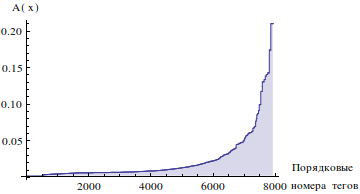
\includegraphics[width=0.5\linewidth]{Dissertation/pics/abstract_words_1}
    \caption{Значения степени абстрактности}
  \end{minipage}
  \label{img:abst_1}
\end{figure}

\begin{figure}[ht]
  \begin{minipage}[ht]{1.0\linewidth}\centering
    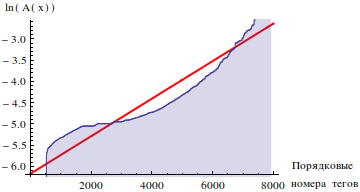
\includegraphics[width=0.5\linewidth]{Dissertation/pics/abstract_words_2}
    \caption{Значения логарифмов степени абстрактности}
  \end{minipage}
  \label{img:abst_2}
\end{figure}


Формулу, определяющую оптимальное значение степени абстрактности p, в окрестность которого попадёт максимальное число искомых тематических тегов, можно представить в следующем виде:

$$p=\exp{M(\{\log{x}|x = \underset{y}\max{(A(y)|y\in p), p \in P})}$$,

где $P$- множество всех наборов ключевых слов, $A(y)$ - абстрактность ключевого слова $y$, $M(x)$ - среднее значение среди $x \in X$

После определения параметра $p$ остается выбрать интервал, содержащий значение $p$.  Например, можно отступить в обе стороны от $p$ на $\epsilon$ и обозначить множество тегов таких, что $A(x) \in [p − \epsilon,p + \epsilon]$, множеством тематических тегов.

\subsubsection{Тестовые испытания модели определения абстрактности и тематических тегов} \label{abstr_test}

\hl{В настоящем разделе результаты тестовых испытаний программной реализации алгоритмов определения степени абстрактности ключевого слова, тематических тегов и тематики документа, а также описываются методы предварительной обработки исходных данных и исправления ошибок.  В качестве таких тестовых данных в работе использован корпус ключевых слов научных публикаций. Коллекция представляла собой вручную составленные списки ключевых слов для публикаций технического и гуманитарного профиля, полученные из различных источников, включая сеть Интернет. По этой причине в этих данных присутствовали ошибки и неточности, полученные при их формировании.}

\hl{По причине того, что данные для тестовых испытаний вводились людьми вручную, было необходимо провести предварительную обработку данных. Предобработка данных - необходимая мера для увеличения точности работы алгоритмов. К мерам, которые применялись для улучшения качества тестовых данных относятся следующие:}

\begin{itemize}
    \item все ключевые слова переводились в нижний регистр;
    \item самые популярные из аббревиатур вручную сопоставлялись со своими развёрнутыми формами;
    \item использовалось несколько разделительных символов;
    \item длинные строки без разделителей разделялись по символам пробелов;
    \item в ключевом слове убирался дефис, если уже существует такое же слово без дефиса.
\end{itemize}

\hl{При этом замечается, что длинные строки без разделителей в действительности могут представлять собой единственное ключевое слово:}

\textbf{[оценка экономического косвенного эффекта от проекта информатизации]}.\

\hl{Или же набор ключевых слов, разделенных по пробелу:}

\textbf{[шахта метан утилизация газогенераторная станция]}.\

\hl{По причине того, что длинные ключевые слова встречаются в данных пренебрежимо мало и в соответствующих вершинах построенных графов мало связей, такие длинные одиночные ключевые слова расценивались как множество однословных ключевых слов.}

\hl{Далее приведен список самых популярных ключевых слов:}

\textbf{наночастицы, инновации, метод конечных элементов, механические свойства, динамика, наноструктуры, прочность, научный потенциал, удар, структура, остаточные напряжения, компьютерное моделирование, управление, модель, оптимизация, мониторинг, образование, математическое моделирование, математическая модель, моделирование}

\hl{Популярность некоторых из этих слов является следствием высокой степени абстрактности (моделирование), но некоторые из них попали в список, потому что некоторая тема может быть популярной (по крайней мере, в рамках данной коллекции). По этой причине теги, относящиеся к этой тематике, могут часто быть использованы в списке ключевых слов (наноструктуры, метод конечных элементов). Способы отделения друг от друга тегов этих двух видов рассматриваются в следующем разделе. Однако, уже сейчас видно, что наивный алгоритм подсчёта количества вхождений тега в коллекцию не даёт необходимого результата.}

\hl{Далее на Рис. \ref{img:abstr_hist} показано количество наборов, обладающих соответствующей долей неуникальных тегов (т.е. тех тегов, которые упоминаются хотя бы в двух наборах из коллекции). Другими словами, для каждого набора подсчитан процент неуникальных ключевых слов и по этим данным построена гистограмма. Важно отметить, что именно неуникальные теги дают возможность дальнейшего анализа. Если бы наборы в основном состояли из уникальных тегов, то использование графов и статистического анализа не привело к достижению каких-либо результатов. Самое популярное значение доли неуникальных тегов - 1.0. Этот факт означает, что теги всех наборов этой категории не являются уникальными, несмотря на то, что коллекция состоит по большей части из уникальных тегов. Примером такого набора является:}

\textbf{[образование, наука, высшая школа, идеология, математика, филология, история, педагогика, биология]}

\begin{figure}[ht]
  \begin{minipage}[ht]{1.0\linewidth}\centering
    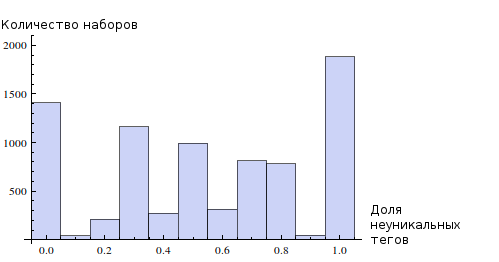
\includegraphics[width=0.5\linewidth]{Dissertation/pics/abstr_hist}
    \caption{Кол-во наборов, с соответсвующей долей неуникальных ключевых слов}
  \end{minipage}
  \label{img:abstr_hist}
\end{figure}

\hl{Зачастую теги наборов такого типа являются очень абстрактными понятиями, что в редких случаях позволяет понять тематику документа. Второе по популярности значение - 0.0. Оно показывает, что существует много наборов, целиком состоящих из уникальных тегов. Причины возникновения таких наборов состоят в следующем:}

\begin{itemize}
    \item ключевые cлова являются слишком узкоспециализированными, например - \textbf{фемтосекундная спектроскопия, лазерные солитоны, дипирролилметаны, подповерхностный радиолокатор};
    \item ключевые слова представлены на другом языке - \textbf{control, sensitivity, equilibria, chaos}.
\end{itemize}

\hl{Следует однако отметить, что основная причина именно в узкой специализации тегов.}

\hl{Между значениями $0.0$ и $1.0$ находится более половины всех наборов. Средняя доля неуникальных тегов по всей коллекции равна $0.53$, то есть, в среднем половина тегов набора встречается в некотором другом объекте коллекции. Типичный набор состоит из нескольких абстрактных тегов, указывающих на общее направление работы и дисциплины, и нескольких тегов, позволяющих понять, о чем конкретно представленный документ.}

\hl{Исходя из перечисленных выше факторов, представляется возможным изучать методы автоматического определения тематики документа и особенности алгоритмов ассоциативного поиска. При этом логичным инструментарием для решения поставленных задач являются графы, которые были введены в предыдущем разделе. Такие графы будут иметь достаточную связность для дальнейшего анализа и возможности примения алгоритмов, которые представлены в предыдущих разделах.}

\hl{Для графа ключевых слов, построенного по данным, были определены компоненты связности и вычислены их размеры. Общее число компонент связности - 1856, что, очевидно, очень много для графа из 17428 вершин. Однако, как показывает график на рис.\ref{img:abstr_hist_2} зависимости номера компоненты и её размера (ось ординат логарифмическая), наибольшая компонента связности содержит более половины всех тегов (11558), а вторая по величине имеет лишь 92 вершины. Начиная с 38 позиции, в компонентах содержится менее 10 вершин.}

\begin{figure}[ht]
  \begin{minipage}[ht]{1.0\linewidth}\centering
    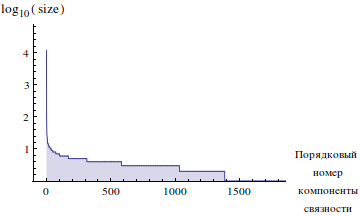
\includegraphics[width=0.5\linewidth]{Dissertation/pics/abstr_hist_2}
    \caption{Распределение размеров компонент связности}
  \end{minipage}
  \label{img:abstr_hist_2}
\end{figure}

\subsubsection{Дополнительный тестовый набор данных}
По причине того, что имеющийся набор данных недостаточно велик, был разработан алгоритм сбора информации о ключевых словах научных статей из сети Интернет. Для этого был использован AP I поисковой системы Яндекс, представляющей функциональные возможности получения поисковой выдачи по запросу. Суть алгоритма в следующем.  

\hl{На вход алгоритма подается одно ключевое слово <KEYWORD>. В поисковую систему отправляется запрос вида <<mime:pdf keywords: /5 <KEYWORD> >>. Этот запрос означа- ет, что необходимо найти документы формата pdf, в которых после слова «keywords:» на расстоянии не более 5 слов находится заданное слово <KEYWORD>. Поисковая система возвращает сниппеты релевантных документов. Ожидается, что значительная часть сниппетов будет содержать список ключевых слов некоторых научных статей. Производится парсинг сниппетов, выделяются кортежи ключевых слов. Собранные ключевые слова добавляются в множество ключевых слов. Тег-запрос добавляется в список использованных ключевых слов. Новое ключевое слово <KEYWORD> выбирается из разности множества всех ключевых слов и множества использованных. Действия алгоритма повторяются до тех пор, пока не будет собрана база ключевых слов достаточного размера.}

\hl{Недостатком программной реализации представленного алгоритма является то обстоятельство, что внешняя поисковая система ограничивает количество запросов в день. По этой причине сбор необходимых данных занимает продолжительное время. Чтобы ускорить процесс, для каждого запроса выкачивается максимально возможное число документов. Как следствие, ключевые слова, по которым строился запрос, встречаются гораздо чаще в собранном множестве ключевых слов. Такой перекос негативно влияет на статистические параметры выборки и ухудшает качество работы реализаций алгоритмов. Другой недостаток состоит в том, что если брать слишком большое число документов, то хвост выдачи становится менее релевантен и в выборку добавляются <<мусорные>> данные.}

\hl{Тем не менее алгоритм решает важную задачу - восполняет недостаток данных. С помощью программной реализации было собрано более 380000 наборов ключевых слов. Для них были проведены методы предобработки данных, описанные в предыдущем пункте. Дополнительно к этому удалялись наборы без разделителей. Вероятнее всего, такие наборы - это обычные предложения со словом keywords, а также наборы, в которых ключевые слова имеют слишком малую длину (обычно в такие сниппеты попадали инициалы авторов статей). Далее это множество данных обозначается как данные из Веб, а первая коллекция именуется чистыми данными.}

\subsubsection{Результаты тестовых испытаний модели определения абстрактности слова}

Самые абстрактные слова, полученные при использования программной реализации описанного выше алгоритма на чистых данных:

\textbf{моделирование, модель, образование, оптимизация, управление, структура, математическая модель, математическое моделирование, мониторинг, прогнозирование, инновации, эффективность, методика, личность, прочность, эксперимент, оценка, история, методы, развитие, анализ, здоровье, инновационная деятельность, культура, качество, свойства, модернизация, синтез, надежность, самоорганизация, адаптация, конкурентоспособность, интеграция, студенты, безопасность, компетенции, взаимодействие, технологии, диагностика, наука, государство, компьютерное моделирование, инновационное развитие, устойчивость, компетентностный подход, динамика, технология, высшая школа, нано-
частицы, метод конечных элементов.}

\hl{В целом получены неплохие результаты по экспертной оценке. Из выделенных слов значительную часть можно назвать абстрактными в некотором смысле. Смешивание помогло избавиться от явных выбросов в каждом из алгоритмов и несколько усреднить результат. Тем не менее, добиться заметного повышения качества не удалось, поскольку представленные алгоритмы имеют одну природу и решают схожие задачи. По этой причине они зачастую ошибаются на некоторых данных одновременно, что влечет за собой ошибку в результатах работы общего алгоритма.}

Результаты работы программной реализации алгоритма на данных из Веб:

\textbf{development, data mining, environment, evaluation, model, management, machine learning, modelling, growth, reliability, neural networks, design, stability, learning, security, uncertainty, clustering, education, performance, modeling, optimization, simulation}

\hl{Для этого набора получены схожие по качеству результату. Однако можно заметить, что некоторые слова продвигаются вверх из-за того, что они были использованы в запросах. Таким словом, например, является термин «machine learning», который не должен был войти в множество абстрактных слов.}

\subsubsection{Результаты тестовых испытаний модели определения тематических тегов}
Значение искомого параметра $p$ в описанном ранее алгоритме оказалось равным $0.0122$.  На чистых данных, для удобства тестирования был выбран интервал $[0.012, 0.013]$. Теги, которые имеют такую степень абстрактности, определены как тематические. Таких ключевых слов обнаружено $65$. В приложении \ref{AppendixB} приводится полный список определенных тематических тегов. Таким образом, алгоритм определил $65$ тегов, из которых $19$ при любых обстоятельствах являются тематическими потому, что это название дисциплин и направлений науки. Еще $13$ тегов субъективно можно считать тематическими. Таким образом точность результата составляет $49.2\%$.

\subsection{Определение смысловой близости для решения задачи поиска эксперта} \label{expert_search_wordsim}
Постановка и решение задачи поиска эксперта рассматривается в главе \ref{expert_search}. Для ее решения возникает необходимость вычислять похожесть между наборами ключевых слов, характеризующих потенциальных экспертов, с ключевыми словами запроса. Для этого, в свою очередь, разработана базовая процедура для определения близости пары ключевых слов, использующая методы и идеи, которые описаны в настоящей главе.

Вычисление смысловой близости пары ключевых слов также основывается на построении графа ключевых слов, введенного в (???). Вершины этого графа соответствуют ключевым словам, а взвешенные ребра отражают факт вхождения слов в один набор. Другим важным понятием является уровень абстрактности ключевого слова, который описан в главе (???). Под абстрактностью понимается степень общности значения слова. Алгоритм определения степени абстрактности по ключевому слову описан в (???). Для вычисления смысловой близости пары ключевых слов используются следующие далее соображения.

\begin{itemize}
    \item \textbf{Чем ближе друг к другу находятся теги в графе, тем больше они схожи по смыслу.} Другими словами, значение семантической близости обратно пропорционально кратчайшему расстоянию между вершинами в графе. За вес ребра принято число наборов из корпуса, в которые входят оба тега. Если $w(i, j) = |{p \in W_X | i \in p \wedge j \in W_X}|$ ­ вес ребра ($W_X$ - множество всех наборов ключевых слов информационной системы), то за длину ребра принята величина $l_0(i, j) = \frac{1}{1+\log(w(i,j))}$ , где $i$, $j$ ­ смежные вершины. Для случая $i = j$ положим $l_0(i, i) = 0$. Следует отметить, что от функции $l_0(i, j)$ достаточно потребовать лишь обратной зависимости от функции $w(i, j)$ . Тем не менее, описанная выше формула позволяет получить лучший результат, чем, например, наивная формула $\frac{1}{w(i,j)}$.
    \item \textbf{Необходимо использовать только статистически важные связи в графе.} Набор ключевых слов к научной публикации не обязан состоять из похожих по смыслу слов. Например, в одном наборе (<<космический аппарат>>, <<упругие элементы>>, <<процесс отделения>>). Замечается, что ключевые слова <<космический аппарат>> и <<упругие элементы>> не должны обладать сильной семантической связью. Поэтому вводится условие: если количество совместных появлений пары тегов меньше порогового значения $t$ , то такая связь в графе не учитывается. Исключением являются те ребра, удаление которых приводит к увеличению числа компонент связности в графе ключевых слов.
    \item \textbf{Пара слов с более высокими степенями абстрактностей должна обладать меньшим значением семантической близости, чем пара узкоспециальных слов.} В качестве примера рассмотрим следующую ситуацию: пара абстрактных по значению тегов («динамика», «кинематика») и пара более узкоспециальных тегов («прибыль», «доход») могут располагаться на одном расстоянии друг от друга в графе. Однако видно, что пара («прибыль», «доход») явно должна иметь большее значение смысловой близости, потому что оперирует более узкоспециализированными тегами. Исходя из этих соображений можно предположить, что семантическая близость должна зависеть от уровней абстрактностей сравниваемых ключевых слов.
    \item \textbf{Пути графа, проходящие через слова с более высокой степенью абстрактности, должны учитываться с меньшим весом.} Слова, обладающие более широким значением, имеют больше связей с другими словами графа. Это обстоятельство приводит к тому, что существует множество пар узкоспециальных слов, которые явно не являются похожими семантически, однако располагаются при этом близко друг к другу в графе. Обычно такое происходит, если пара слов имеет общую вершину с высокой степенью абстрактности. Например, пара тегов («ленивые вычисления», «оценка максимального правдоподобия») находятся близко друг к другу из­за их связей с тегом «машинное обучение», который является более общим понятием. Можно при этом заметить, что на самом деле слова этой пары далеки друг от друга семантически. По этой причине возникает необходимость «перевзвесить» ребра графа. Обозначим степень абстрактности ключевого слова $x$ за $A(x)$. Величина $A(x)$, исходя из введенного в главе (???) определения, не превышает  1. Положим теперь длину ребра равной $l(i, j) = \exp(\frac{l_0(i, j)}{\log(A(i))\log(A(j))})$. Таким образом, чем выше степени абстрактности вершин, инцидентных данному ребру, тем больше длина этого ребра. Длина кратчайшего пути между вершинами $v_x, v_y$ принята за $L(v_x,v_y)$ . Экспонента в формуле делает значение $l(i, j)$ не меньшим, чем 1.
    \item \textbf{Чем больше различных связей (путей) между вершинами в графе, тем больше уровень семантической близости.} При этом дополнительную информацию дают веса ребер. Это следует из того, что если два тега связаны тяжелым ребром или путь между ребрами имеет большой вес, то такие теги будут более близки по смыслу, чем аналогичная пара с легкими ребрами. В этой связи возникает необходимость решения задачи определения максимального потока между двумя вершинами графа. В классической постановке требуется для пары вершин, называемых источником и стоком, транспортной сети найти такой поток из источника в сток, что его величина будет максимальна. На граф тегов эта задача переносится очевидным образом, если ребра принять за двунаправленные, а за пропускную способность ребра ­ его вес. При этом пропускная способность считается отдельно для каждого из направлений. Пусть максимальный поток между вершинами $v_x, v_y$ равен $MaxFlow(v_x, v_y)$. Максимальной вместимостью вершины назовем сумму весов ребер, входящих в нее. Обозначим максимальную вместимость вершины $i$ за $C(i)$. Тогда за $F(v_x,v_y)$ примем величину, равную $\frac{MaxFlow(v_x,v_y)}{min(C(v_x), C(v_y))}$. В этом случае $F(v_x,v_y)$ показывает, насколько использована пропускная способность канала между вершинами. Максимум, равный единице, достигается, если пропускная способность использована полностью. В частности, $F(vx,vx) = 1$.
\end{itemize}

Учитывая перечисленные выше cоображения, формула близости между парой ключевых слов $x$ и $y$ вводится следующим образом:

$$ WordSim_{expert}(x, y) = \frac{F(v_x, v_y)}{L(v_x, v_y)}, $$

где $v_x$ и $v_y$ - пара вершин в графе ключевых слов, соответствующая ключевым словам $x$ и $y$.


\subsection{Тестовые испытания} \label{test_sect}
В настоящем разделе описаны результаты тестовых испытаний программных реализаций описанных ранее алгоритмов. В качестве тестовых данных были использованы корпусы ключевых слов для научных публикаций, собранных из сети Интернет. Использовалась также информация из социальной сети Вконтакте, а именно - были выкачаны посты (публичные сообщения из групп и страниц пользователей), часть из которых помечены хэштегами. В процессе сбора данных проводился парсинг текстовых данных на предмет наличия в них наборов ключевых слов. Точное решение этой задачи не является предметом исследования данной работы (???), поэтому для парсинга данных были использованы наивные подходы, которые, тем не менее, позволяют собрать корпус достаточного размера и качества  для проведения дальнейшего анализа.
В конечном итоге собрано два объемных набора данных:
\begin{itemize}
    \item 329.000 наборов для русского языка;
    \item 3.069.000 наборов хэштегов из сети Вконтакте.
\end{itemize}
Далее приведены примеры наборов ключевых слов из обоих источников. Наборы ключевых слов научных публикаций:

    \textbf{[топонимический концепт, языковое сознание, когнитивная база, прецедентность, апеллятивация]}\

    \textbf{[вариабельность сердечного ритма, гребля на каноэ, вегетативный тонус]}\
    
    \textbf{[архитектуры, деформации, геологическая среда, сфера взаимодействия]}

Наборы хэштегов из социальной сети:

    \textbf{[electro\_pop, dance, fresh, music, new\_zealand]}\

    \textbf{[vitaminhealth, oxygenwater, waterhealth]}\

    \textbf{[bodyfan, питание, bodyfanпитание, bodyfanmotivation, motivation, bodybuilding, фитнес, gym, спорт, мотивация, зож]}

\subsubsection{Определение семантической близости с использованием графов ключевых слов}
Программные реализации описанных в предыдущих главах алгоритмов были применены к собранным данным. Далее на рисунке \ref{img:sim_1} представлены ближайшие соседи для слов <<федерация>> и <<регионы>> в графе ключевых слов.

\begin{figure}[ht]
  \begin{minipage}[ht]{0.49\linewidth}\centering
    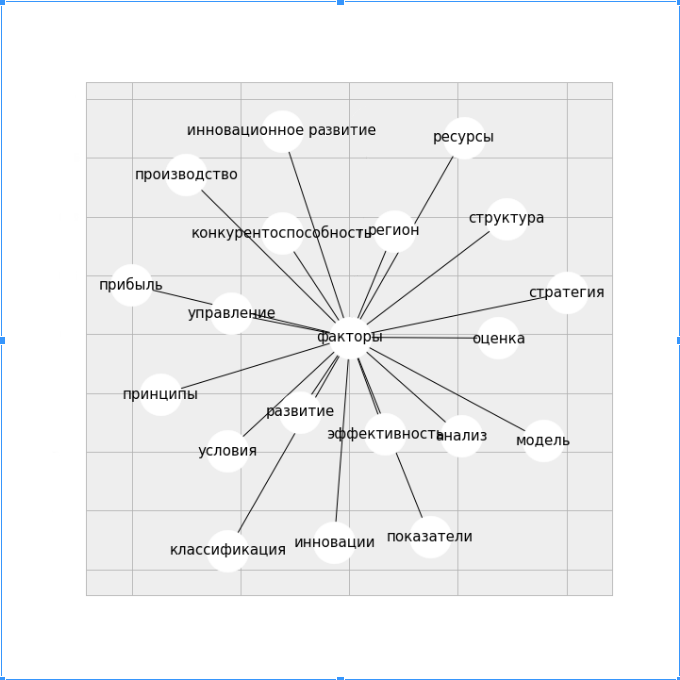
\includegraphics[width=1.0\linewidth]{Dissertation/pics/factory_sim} \\ а)
    \caption{Соседи вершины <<факторы>> в графе ключевых слов}
  \end{minipage}
  \hfill
  \begin{minipage}[ht]{0.49\linewidth}\centering
    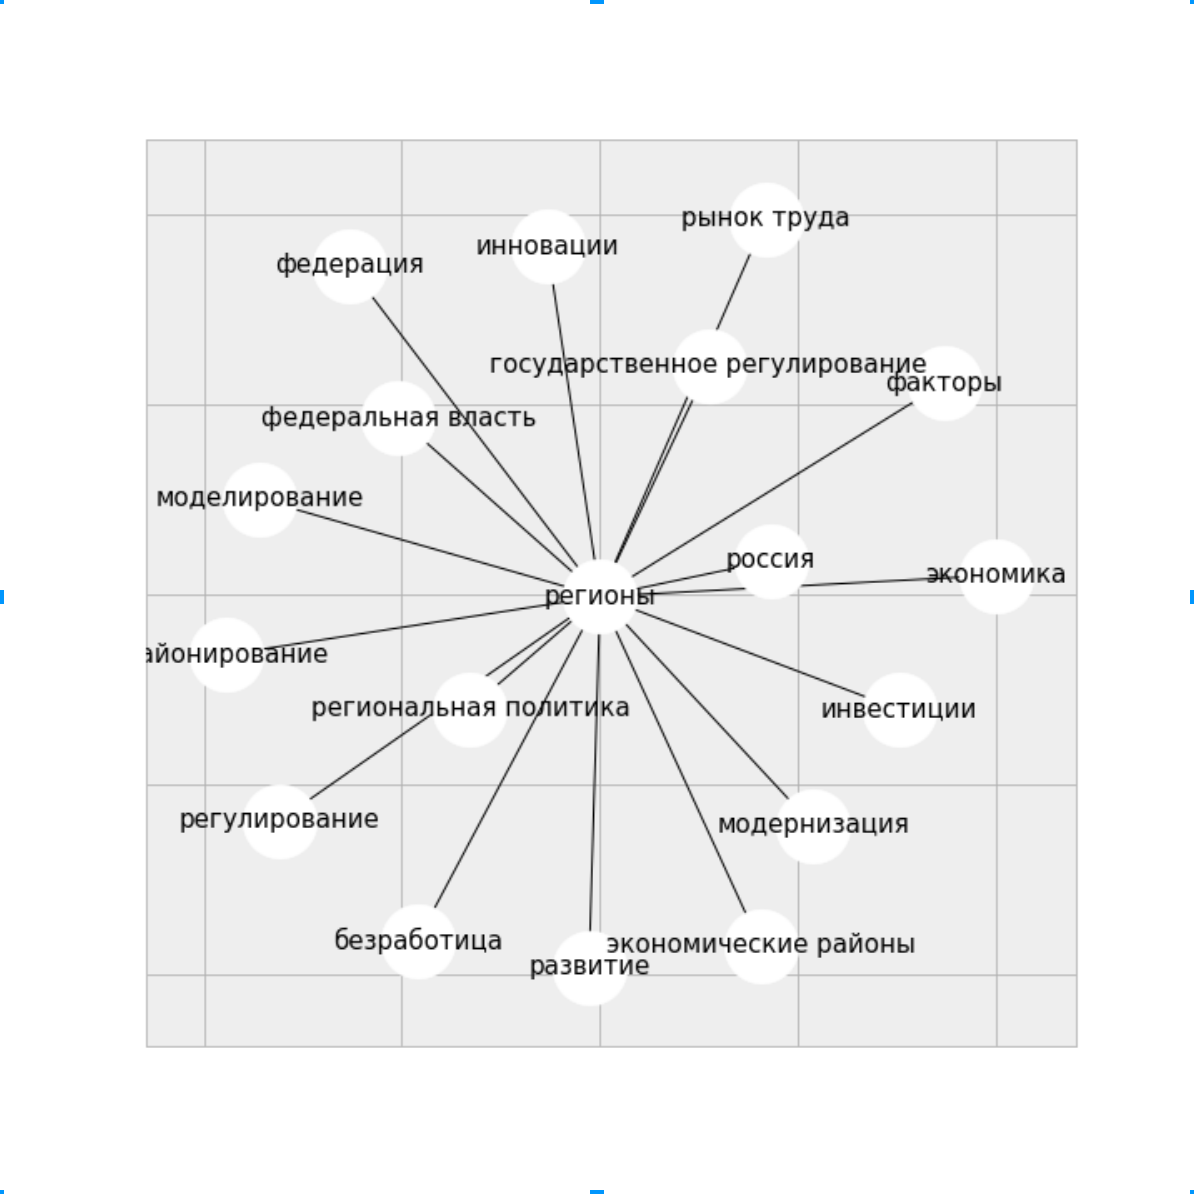
\includegraphics[width=1.0\linewidth]{Dissertation/pics/regiony_sim} \\ б)
    \caption{Соседи вершины <<регионы>> в графе ключевых слов}
  \end{minipage}
  \label{img:sim_1}
\end{figure}

На рисунках выше видно, что графа ключевых слов не хватает для определения семантической близости пары слов: видно, что существуют связи такие, как <<факторы-модель>>, <<регионы-экономика>>, которые не обладают явной смысловой связью. Применение методов построения усеченного контекстного графа дает значительное улучшение качества классификации пар ключевых слов на семантически близкие и далекие. Далее указаны примеры найденных пар ключевых слов, близких по смыслу:

\textbf{β-адреноблокаторы   -   бета-адреноблокаторы}

\textbf{новые виды   -   новый вид}

\textbf{орви   -   острые респираторные вирусные инфекции}

\textbf{текущий уровень информационной безопасности   - политика информационной безопасности}

\textbf{умения   -   навыки}

\textbf{образное мышление   -   художественный вкус}

\textbf{хехцир   -   khekhtsyr}

\textbf{рынок банковских услуг   -   банковский рынок}

\textbf{тромболизис   -   тромболитическая терапия}

\textbf{параллельные алгоритмы   -   параллельное программирование}

\textbf{феминность   -   фемининность}

\textbf{полином  -  многочлен}

\textbf{корень  -   корни}

\textbf{primerun  -  примерун}

\textbf{fvk  -  fotovideoclub}

\textbf{еврореволюция  -   єврореволюція}

\textbf{silk\_plaster    -  шелковая\_штукатурка}

Интересным фактом является определение похожих слов для заданного многозначного слова. В то время как граф в графе ключевых слов соседями для слова <<орган>> являются слова <<государство>>, <<сибирь>>, <<контроль>>, <<циркуляция>>, <<управление>>, в контекстном графе ближайшими являются слова <<музыковедение>>, <<организм>>, <<отклонение>>, <<делегирование полномочий>>, <<объект контроля>>. Таким образом восстанавливается не только значение слова, связанное с юриспруденцией, но и близкие слова для значения из области музыки (<<музыковедение>>) и биологии (<<организм>>).

На рисунке \ref{img:sim_2} изображены несколько ближайших контекстно близких слов для слова <<студенты>> (отмечается, что полное множество соседей вершины слишком велико, чтобы его изобразить):

\begin{figure}[ht]
  \begin{minipage}[ht]{1.0\linewidth}\centering
    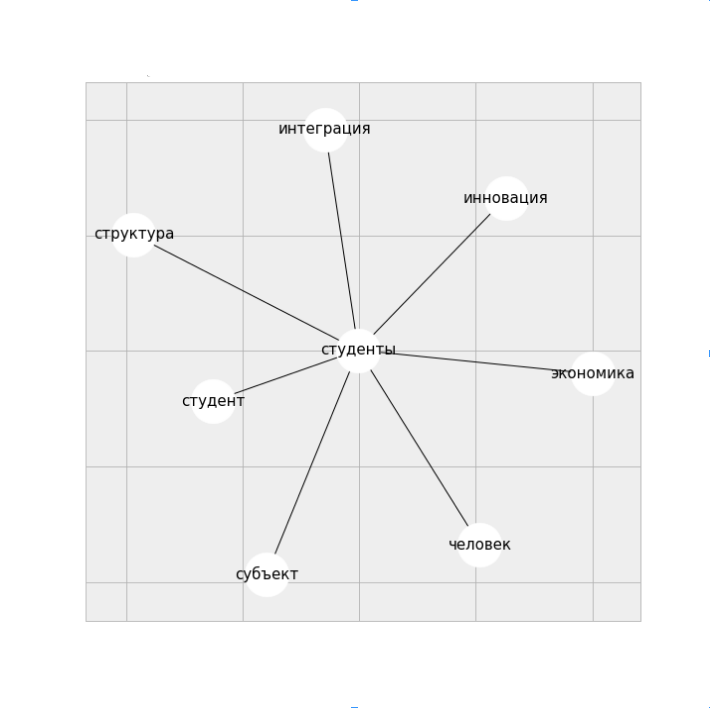
\includegraphics[width=1.0\linewidth]{Dissertation/pics/students_sim}
    \caption{наиболее близкие слова для слова <<студенты>> в контекстном графе}
  \end{minipage}
  \label{img:sim_2}
\end{figure}


\subsubsection{Построение кластеров семантически похожих ключевых слов}

Описанный ранее алгоритм кластеризации контекстного графа позволяет удалять недостаточно надежные связи между словами, полученные с помощью алгоритма определения близости по контекстному графу, и, наоборот, добавлять новые ребра между семантически похожими парами слов. 

Кластер для слова <<студенты>> изображен на рисунке \ref{img:clust_1}

\begin{figure}[ht]
  \begin{minipage}[ht]{1.0\linewidth}\centering
    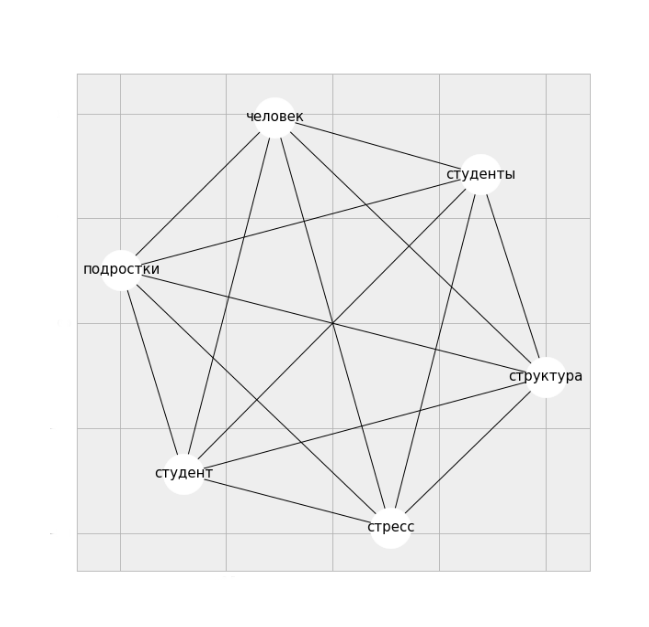
\includegraphics[width=1.0\linewidth]{Dissertation/pics/students_cluster}
    \caption{кластер, содержащий слово <<студенты>>}
  \end{minipage}
  \label{img:clust_1}
\end{figure}

Можно заметить, как в результате кластеризации были разорваны связи <<студенты-экономика>>,  <<студенты-инновации>>, вместо которых на первый план вышли связи <<студенты-подростки>>. Отмечается также, что выбранный метод кластеризации графа может допускать ошибки. Например, в случае с парой <<студенты-структура>>, которая была как в усеченном контекстном графе, так и в кластере слова студент.

Для интегральной проверки качества была выбрана следующая методика.

\begin{enumerate}
    \item Набирается набор пар ключевых слов, для которых можно  определить их высокий уровень семантической близости посредством детерминированного алгоритма (положительные примеры). Пара слов определяется близкой по смыслу, если выполняется хотя бы одно из условий:
    \begin{enumerate} 
        \item одно ключевое слово является аббревиатурой для другого;
        \item расстояния Левенштейна между парой невелико.
    \end{enumerate}
    \item К зафиксированным семантически похожим парам слов добавляются отрицательные примеры, т.е. пары слов, которые не являются близкими по смыслу. Для этого проводятся следующие шаги:
        \begin{enumerate}
            \item если пара слов $(a,b)$ определена на первом шаге как пара похожих слов, то для слова aберется $k$ случайных соседей $c_1, c_2, \dots,c_k$ из графа ключевых слов на расстоянии, не превышающем 2; 
            \item все пары $(a,c_i)$ определяются как отрицательные примеры.
        \end{enumerate}
    \item Положительные и отрицательные примеры составляют тестовую выборку. После чего для всех пар тестовой выборки вычисляется близость, по формулам описанным выше, а также подбирается порог, по которому в зависимости от вычисленного значения близости пара относится либо к классу семантически близких пар, либо к классу семантически далеких.
    \item По оценкам классификатора и тестовой выборке считается F-мера, которая и является показателем качества алгоритма.
\end{enumerate}

В результате тестирования программной реализации алгоритма получено высокое  по отношению к реализованным в [???] алгоритмам значение F-меры - 0.82. Проведение аналогичного теста для алгоритма определения близости лишь с помощью анализа частотности встречаемости пары слов дает результат 0.67, таким образом, методы, описанные в данной работе существенно улучшают качество определения семантической похожести. Отмечается, что выбранный способ тестирования имеет очевидный недостаток: среди положительных примеров очень редко встречаются пары смысловых синонимов, напротив, они могут попадать в пары отрицательных примеров. Тем не менее, по экспертной оценке увеличение качества на описанной ранее тестовой выборке влечет улучшение качества классификации и более сложных пар ключевых слов, таких как  пар <<синоним>>-<<синоним>> или <<слово>>-<<перевод слова на другой язык>>.

\subsubsection{Тестирования алгоритмов определения абстрактности слова}
Самые абстрактные слова, полученные при использования программной реализации
описанного выше алгоритма на чистых данных:

моделирование, модель, образование, оптимизация, управление, структура, математическая модель, математическое моделирование, мониторинг, прогнозирование, инновации, эффективность, методика, личность, прочность, эксперимент, оценка, история, методы, развитие, анализ, здоровье, инновационная деятельность, культура, качество, свойства, модернизация, синтез, надежность, самоорганизация, адаптация, конкурентоспособность, интеграция, студенты, безопасность, компетенции, взаимодействие, технологии, диагностика, наука, государство, компьютерное моделирование, инновационное развитие, устойчивость, компетентностный подход, динамика, технология, высшая школа, наночастицы, метод конечных элементов.

В целом получены неплохие результаты по экспертной оценке. Из выделенных слов значительную часть можно назвать абстрактными в некотором смысле. Смешивание помогло избавиться от явных выбросов в каждом из алгоритмов и несколько усреднить результат. Тем не менее, добиться заметного повышения качества засчет этого не удалось, поскольку представленные алгоритмы имеют одну природу и решают схожие задачи. По этой причине они зачастую ошибаются на некоторых данных одновременно, что влечёт за собой ошибку в результатах работы общего алгоритма.

Результаты работы программной реализации алгоритма на данных из Веб:

development, data mining, environment, evaluation, model, management, machine learning, modelling, growth, reliability, neural networks, design, stability, learning, security, uncertainty, clustering, education, performance, modeling, optimization, simulation

Для этого набора получены схожие по качеству результату. Однако можно заметить, что некоторые слова продвигаются вверх из-за того, что они были использованы в запросах. Таким словом, например, является термин «machine learning» , который не должен был войти в множество абстрактных слов.

\subsubsection{Апробация автоматического тематического классификатора}
...
\subsection{Выводы}
По результатам исследований, результаты которых представлены в разделе \ref{test_sect}, построены модели определения близости по корпусу наборов ключевых слов, опирающиеся на методы из теории графов. Для данных моделей представлены алгоритмы и созданы программные реализации этих алгоритмов. Реализации были протестированы на двух коллекциях наборов ключевых слов и был получен относительно высокий уровень качества результатов. Кроме того, была разработана модель кластеризации ключевых слов, опирающаяся на введенные графовые модели представления коллекций ключевых слов и на построенную по этим графам меру схожести для пары слов. Программная реализация процедуры кластеризации также протестирована, для нее был получен высокий уровень качества определения кластеров схожих ключевых слов.
\textbf{??? добавить текст про тематический классификатор}
Недостатком работы может являться большое число параметров, которое необходимо настроить. В качестве дальнейшего направления в изучении данной области автор настоящей дисертации считает целесообразным применения методов машинного обучения для построения меры близости между ключевыми словами. Такой шаг поможет избавиться от значительной части параметров описанных в предыдущих главах моделей, предоставив возможность настройки этих параметров в автоматическом режиме.

\section{Использование методов машинного обучения для улучшения модели близости слов}
В настоящей главе рассматриваются методы улучшения качества определения семантической близости для пары ключевых слов с помощью методов машинного обучения с учителем. Далее в тексте подробно описывается сведение рассматриваемой задачи к задаче классификации, то есть к задаче определения целевой метки заданного объекта из заранее сформированного множества меток. Обучение с учителем подразумевают использование обучающей выборки - множества объектов, для которой известны истинные целевые метки. Эта выборка необходима для тренировки модели машинного обучения. Обученная модель машинного обучения применяется к произвольному объекту системы и выдает предсказанную целевую метку.

\hl{Сбор обучающего набора данных является обычно трудоемкой и дорогой работой: как правило для процесса требуется как минимум несколько экспертов в направлении, для которого собираются тренировочное множество. Более того, для некоторых задач, в число которых входит и задача определения семантической близости пар ключевых слов, является сложным даже правильно составить инструкцию для экспертов для правильной оценки примеров. Это происходит по причине того, что семантическая близость - субъективная величина и сильно зависит от области применения, контекста, человека и задачи. Например, слово <<стол>> может быть близким по смыслу для слова <<стул>> из бытовых соображений. В то же время если бы эти два слова были синонимами (а следовательно взаимозаменяемыми) в информационной системе, представляющей интернет-магазин, продающий мебель, то имела бы место ситуация, когда пользователь ищет один из этих предметов, а в поисковой выдаче получает другой, что является недопустимым. Рассмотренные в следующих далее разделах алгоритмы сбора обучающего множества призваны разрешить обозначенные проблемы.}

\hl{Автором настоящей диссертации были разработаны два метода получения обучающих примеров без задействия в процесс экспертов. Первый из них включает в себя набор эвристических алгоритмов создания обучающей выборки. Второй является полностью автоматическим методом и строится исключительно при помощи описанных в предыдущих главах графовых моделей представления данных. Важнейшим преимуществом этого метода является его универсальность и применимость не только к задачам определения семантической близости, но и к любым другим задачам, в которых объекты системы представляются в виде некоторого графа и имеется необходимость в классификации отношений между парой объектов. Также универсальность проявляется в том, что выборка строится непосредственно по данным и не использует никакие внешние источники. Это позволяет определить отношение близости специфичные для конкретной системы. Другое преимущество метода в возможности использовать эффективные модели машинного обучения с учителем, вместо более слабых моделей без учителя, которые, к тому же представляется сложным валидировать без обучающих примеров.}

Задача классификации для определения семантической близости пары ключевых слов формулируется следующим образом. Пусть $X=\{x_i\}_{i=1}^N$ - множество пар ключевых слов. $x_i=(x_l,x_r)_i$ - пара ключевых слов, где $x_l,x_r$ - левое и правое слова из пары. $Y={0,1}$ - множество меток. Нулевое значение соответствует отсутствию семантической близости для пары ключевых слов, а единичное, напротив, сильной смысловой связи. Поскольку $Y$ состоит только из двух элементов, то такая задача называется задачей бинарной классификации. $X^l=(x_i,y_i)_{i=1}^l$, где $x_i \in X, y_i \in Y$ - обучающающая выборка. Далее по обучающей выборке строится классификатор $a: X\rightarrow Y$

Процесс сбора обучающей информации является одним из важнейших этапов обучения эффективной модели определения семантической близости. Сложность этого процесса заключается в невозможности точно формализовать для пары ключевых слов отношения <<являются семантически близкими>> и <<не являются семантически близкими>>. Во многих случаях определение смысловой близости зависит от решаемой задачи, поэтому обучающие выборки для одной задачи могут не подходить для обучения моделей из другой. Например, пары ключевых слов <<математика>> и <<математическая статистика>> (связаны отношением гиперонимии (<<математическая статистика>> является разделом <<математики>>), что влечет некоторую смысловую близость между понятиями. C другой стороны, если рассматривать задачу поиска документов системы по ключевым словам, то при заданном пользователем запросе <<информатизация,математика,вектор информатизации,информационные технологии,mathematica>>.  Для данного запроса ключевое слово <<математическая статистика>> не подходит по контексту данного запроса, кроме того, это ключевое слово является более узким по смыслу, чем <<математика>> и поэтому шансы пользователя получить релевантные запросу документы минимальны: если даже пользователь предполагал какую-то более узкую область, нет никаких оснований полагать, что это именно <<математическая статистика>>, а не, например, <<вычислительная математика>>. Обратная ситуация, когда пользватель ввел запрос <<математическая статистика, статистические тесты>>, то поиск в документах предположительно синонимичного слова <<математика>> также может привести к ухудшению выдачи: в результате этого действия, в выдачу вероятно попадут документы слишком общего смысла, такие как статьи про математику как науку.

Другим примером неоднозначности в определении семантической близости может служить различия в тематической направленности систем, в которых используются модели определения смысловой близости. Для наукометрических систем пара ключевых слов <<математическая статистика>> и <<вычислительная математика>> вряд ли должны иметь большое значение метрики смысловой близости, потому что в рамках такой системы эти два понятия представляют два совершенно различных направления математики. В то же время в системах более общей направленности, где могут присутствовать документы любого рода (а не только научные публикации), данная пара ключевых слов должна иметь более высокий уровень семантической похожести, поскольку для такой системы все термины относительно небольшого раздела <<математика>> могут считаться близкими по смыслу.

Качество модели определения семантической близости в данном случае целиком определяется двумя составляющими: параметрами обучающей выборки (качеством, разнообразием и количеством обучающих примеров) и эффективностью выбранного алгоритма машинного обучения. 

Лучшим алгоритмом для решения поставленной задачи бинарной классификации является модель градиентного бустинга на решающих деревьях XGBoost \cite{xgboost}. В ходе обучения происходит последовательное построение композиции решающих деревьев, каждое следующее дерево при этом стремится максимально уменьшить ошибку уже построенной части ансамбля. Анализ эффективности выбранной модели, сравнения модели XGBoost с другими существующими моделями и тестовых испытания представлены в следующих далее разделах. 

\subsection{Методы формирования обучающей выборки}
В данном разделе описывается два разработанных способа получения обучающего набора данных. Первый из них использует различные эвристические идеи о том, как с помощью простых детерминированных процедур и, в некоторых случаях, внешних открытых наборов данных получать примеры близких по смыслу пар ключевых. Такие методы имеют высокий уровень точности, но слабое покрытие пространства пар ключевых слов системы. Второй способ заключается в использовании теоретико-графовых алгоритмов для, способных выдавать примеры семантически близких и далеких пар объектов, основываясь на графовой структуре представления данных.

\subsubsection{Эвристические методы}
Идейно различаются два типа алгоритмов сбора обучающей выборки. Первый из них заключается в использовании некоторых внешних словарей и дальнейшая фильтрация этих словарей по тем словам, которые присутствуют в информационной системе. Второй способ сначала использует некоторый генеративный алгоритм (например, составляется большое множество пар ключевых слов, которые встретились внутри одного набора). Далее это множество фильтруется с помощью некоторого алгоритма и те пары, которые прошли фильтрацию, объявляются близкими по смыслу. Примером такого алгоритма может быть алгоритм, считающий расстояние Левенштейна. Если редакторское расстояние не превосходит 1, то слова имеют очень схожее написание и  весьма вероятно, что они близки по смыслу. Такая процедура фильтрует значительную часть пар, но те пары, которые прошли фильтрацию, почти всегда  имеют высокую степень смысловой близости. Таким образом каждый такой фильтр получает примеры близких по смыслу пар слов с высокой точностью, но низкой полнотой. 

Были разработаны следующие эвристические методы сбора обучающей выборки
\begin{itemize}
    \item Поиск простых аббревиатур. Ключевые слова системы разделяется на понятия, содержащие ровно одно слово - аббревиатуры, и понятия, содержащие более одного слова- расшифровки аббревиатур. Далее для каждого слова из множества аббревиатур и каждого словаиз множества расшифровок проверяется, действительно ли данная расшифровка является расшифровкой для данной аббревиатуры. Другими словами проверяется, что существуют такие префиксы слов расшифровки, которые могут полностью покрыть аббревиатуру. Если соответствие установлено, то пара аббревиатура-расшифровка добавляется в список пар-кандидатов. Далее к парам-кандидатам приписываются частоты входящих в них ключевых слов. Для каждой аббревиатуры берется не более 5 наиболее частотных вариантов расшифровок. Пары, прошедшие данную фильтрацию, формируют окончательное обучающее множество аббревиатур;
    \item поиск скобочных аббревиатур. Иногда при написании ключевых слов-аббревиатур в скобках указывается правильная расшифровка для данной аббревиатуры. Это позволяет собрать дополнительные пары аббревиатура-расшифровка для обогащения множества обучающих примеров;
    \item поиск разных форм одного слова. С помощью пакета обработки естественного языка NLTK для каждого слова в системе рассматриваются различные его формы. Если одна из форм также присутствует в множестве всех ключевых слов, то пара слово-форма добавляется в обучающее множество;
    \item поиск похожих по написанию слов. Рассматриваются все пары слов, расстояние левенштейна между которыми равно 1. Эти пары добавляются в обучающее множество;
    \item поиск переводов с одного языка на другой. Данный метод использует API сервиса Яндекс.Переводчик и собирает варианты переводов ключевых слов с русского языка на английский;
    \item поиск синонимов в тезаурусе WordNet. Были использованы пары синонимов и пары гипоним-гипероним. Кроме поиска по англоязычным синсетам был использован двухступенчатый подход определения синонимов: русскип слова переводились средствами сервиса Яндекс.Переводчик на английский язык, а затем поиск проводился уже по английским версиям слов;
    \item использование открытых источников синонимов. Из словарей синонимов, доступных в сети Интернет, выделяются те пары, слова которых присутствуют в множестве ключевых слов.
\end{itemize}

Данные методы сбора данных позволяют собрать положительные примеры для обучения, то есть примеры пар ключевых слов, являющиеся семантически похожими. Однако, для правильного обучения модели необходимы также и отрицательные примеры. С помощью небольших модификаций эвристических алгоритмов сбора положительных примеров можно получить алгоритмы для сбора отрицательных примеров. Были использованы следующие идеи:
\begin{itemize}
    \item поиск антонимов в тезаурусе WordNet. Аналогично поиску синонимов был проведен поиск антонимов в базе WordNet. Также были использованы пары слов, расстояние в дереве WordNet между которыми превышает 2;
    \item неправильные расшифровки для аббревиатур. Рассматриваются те аббревиатуры, для которых были найдены правильные расшифровки. Этим аббревиатурам ставятся в пару случайные многословные ключевые слова, которые точно не являются правильными расшифровками;
    \item использование открытых источников антонимов;
    \item случайные пары ключевых слов. Для каждого ключевого слова, для которого в выборке присутствуют положительные примеры, были взяты случайные ключевые слова в пару. На одно слово было сгенерировано не более, чем 10 пар. Данный метод был использован по следующим соображениям. Предполагается, что для каждого ключевого слова существует константное число близких по смыслу ключевых слов. То есть если в достаточно большой информационной системе начинает расти количество ключевых слов, то кол-во слов, похожих на данное слово, не будет расти линейно по числу уникальных слов системы. В то же время количество пар растет квадратично, а количество пар для заданного слова - линейно, а это означает, что если взять для заданного слова в пару случайное слово, то эта пара не будет связана семантически. При этом важным является подбор доли случайных пар. Если эта доля мала, то в выборке не будет достаточного разнообразия отрицательных примеров. Если же доля слишком велика, то случайные пары будут вносить слишком большой вклад в обучение модели, что не является правильным вариантом, потому что в случайные отрицательные пары не настолько качественны, как, например, антонимы из словаря. Оба этих случая приводят к ухудшению качества модели определения семантической близости.
\end{itemize}

В результате работы программных реализаций алгоритмов было собрано 234974 положительных и 1175610 отрицательных примеров.

Обучение моделей на эвристически подобранных выборках имеет заметные недостатки:

\begin{itemize}
    \item Смещение в данных. Для наилучшего обучения классификаторы необходимо, чтобы объекты обучающей выборки выбирались из распределения тех объектов, на которых классификатор будет работать в реальной системе. Рассмотрим данную особенность на следующем тривиальном примере. Допустим, что все пары ключевых слов системы делятся на Аббревиатуры (то есть пара аббревиатура - расшифровка аббревиатуры) и Переводы (слово на русском языке - его перевод на английский). Если Аббревиатур в системе 10\%, то и в обучающем подмножестве должно Аббревиатур должно быть 10\%. Если же аббревиатур при обучении будет значительно больше (например, 70\%), то модель начнет усиленно использовать те факторы, которые повышают ее качество на аббревиатурной части выборки, потому что это лучшим образом оптимизирует функцию потерь. Однако, в момент применения модели, к ней на вход будет поступать только 10\% аббревиатур и 90\% переводов и очень вероятно, что факторы, используемые моделью не будут оптимальны для классификации переводов и тем самым это улучшит качество реальных решаемых задач данным классификатором.  

Другой недостаток смещения заключается в том, что если перегрузить обучающую выборку примерами неправильных переводов, то это негативно отражается на предсказанных уровнях близости во время этапа применения модели. То есть это понизит средний уровень близости между переводами в системе. Это понижение приведет к тому, что если для данного ключевого слова (<<MSU>>) есть и правильная аббревиатура (<<Moscow State University>>), и правильный перевод (<<МГУ>>), то из-за рассмотренной манипуляции с обучающей выборкой, значимость перевода будет понижена. В конечном счете может оказаться, что согласно модели, все аббревиатуры лучше всех переводов. Такое поведение не очевидно и не основывается на реальной работе информационной системы. Такой сценарий возможен, поскольку положительные и отрицательные примеры берутся из разных источников, поэтому степень покрытия ими всего разнообразия пар ключевых слов, а также возможность контролировать нужную долю положительных примеров остается под вопросом;
    \item модель настраивается не под конкретную задачу и не под конкретные данные системы. Если, например, слова <<объединять>> и <<интегрировать>> попали в один внешний словарь синонимов общего назначения, то внутри информационной системы, направленной на изучение технических наук, эти слова определяют две различные математические операции. Также может случиться, что в узкоспециальных областях эти могут являться слишком общими по смыслу, чтобы быть похожими. Примером такой пары может быть <<ураган>> и <<тайфун>>. Для пользователя, например, социальной сети эти слова действительно похожи. Однако, в рамках системы, изучающей различные природные явления, слова имеют важные смысловые отличия. И чем специфичнее тематика системы, чем четче прослеживается различия между словами, который с точки зрения словарей общей направленности, очень похожи;
    \item сложность процесса сбора обучающей выборки. Для каждой системы нужны свои наборы эвристик, что затрудняет внедрение таких классификаторов повсеместно.
    \item ошибки в выборке. По причине того, что частично выборка состоит из случайных примеров, вероятно, что существует небольшое число пар, которые ошибочно промаркированы отрицательными. Это может понизить качество обученной модели. Помимо этого могут возникать ошибки второго рода. Например, если внешний сервис, предоставляющий переводы для слов и фраз допустил ошибку, то в множество положительных примеров попадет неправильный перевод для слова.
\end{itemize}

\subsubsection{Автоматические методы}
\hl{Для устранения недостатков, описанных в предыдущей главе, был разработан метод автоматической генерации обучающей выборки. Суть данного метода заключается в использовании графовой структуры данных для получения обучающих примеров.}

\hl{Первым шагом метода является искусственная модификация текстовых данных. Для этого вводится специальный символ @, который не используется в написании ключевых слов. Далее фиксируется некоторое дискретное распределение. В первой версии программной реализации данного алгоритма было использовано дискретное равномерное распределение из двух значение и далее для простоты основная суть и мотивация алгоритма будут изложены именно для этого распределения.}

\hl{Рассматриваются ключевые слова, встретившиеся хотя бы $N$ раз в системе. $N$ выбирается таким образом, чтобы отсеять те слова, для которых в системе недостаточно информации, но при этом множество множество  ключевых слов прошедших фильтрацию оставалось достаточным (десятки тысяч слов) для дальнейшего обучения: в сгенерированную выборку попадут только эти слова. В программной реализации параметр $N$ был принят равным $10$. }

\hl{Пусть $w_i^k$ обозначает вхождение $i$-го ключевого слова системы в $k$-ый набор ключевых слов. Для каждого вхождения слова $w_i^k$, прошедшего фильтрацию, в наборы ключевых слов, берется число $d$ из выбранного распределения. После этого к вхождению слова $w_i^k$ приписывается суффикс $@d$, то есть добавляется специальный символ @ и ставится число $d$ из распределения. Таким образом, данная операция производит новое ключевое слово. Рассмотрим, например, следующие наборы ключевых слов:}

\textbf{[резание металлов, высокоскоростное фрезерование]}\

\textbf{[резание металлов, аморфизация, адгезия, наростообразование]}\

\textbf{[резание металлов, адгезия, высокосоростное фрезерование]}\

После описанной выше процедуры эти наборы ключевых слов могли перейти в:

\textbf{[резание металлов@0, высокоскоростное фрезерование@1]}\

\textbf{[резание металлов@1, аморфизация@1, адгезия@0, наростообразование@1]}\

\textbf{[резание металлов@1, адгезия@0, высокосоростное фрезерование@1]}\

\hl{Таким образом, каждое слово $w$, прошедшее первичную фильтрацию по частоте встречаемости, переходит в два новых слова $w@0$ и $w@1$. И во всей коллекции наборов ключевых слов теперь используются модифицированные версии $w@0$ и $w@1$. Это пара слов $w@0$ и $w@1$ является, по сути, одним и тем же словом, и, следовательно, может быть положительным обучающим примеров для выборки. Поскольку слово $w$ в исходных данных встречалось достаточное количество раз. После того, как модифицирован весь объем предоставленных данных, происходит построение описанных в предыдущих главах графов, выполняются процедуры подсчета факторов. Задачей модели машинного обучения в этом случае будет восстановить по графовым связям факт идентичности разных версий одного слова. Если модель успешно обучена искать различные версии одного и того же слова, то при применении модели на реальных данных, появляется возможность классифицировать пары синонимов и, более общо, определять семантическую связь между ключевыми словами.  Это происходит по той причине, что синонимичная пара на самом деле обладает тем же свойством, каким обладает искусственно полученные положительные примеры выборки: при замене одного слова на другое не меняется смысл всего набора. А значит стоит ожидать, что статистические и графовые связи между искусственной парой слов и синонимичной парой во многом похожи.}

\hl{Но в рамках описанной модели генерации обучающих примеров возникает эффект, из-за которого появляются статистические различия между созданными искуственными парами и настоящими синонимичными словами. Дело в том, что при наивном выборе в равномерного дискретного распределения из двух элементов в качестве генерирующего распределения, зачастую слова $w@0$ и $w@1$ встречаются приблизительно равное число раз. При этом настоящие синонимичные пары таким свойством обладать не обязаны. Например, ясно, что слово "зарплата" будет употребляться гораздо чаще, чем устаревший синоним "жалованье". Поэтому для моделирования искусственной обучающей выборке необходимо взять более сложное распределение. В качестве такового было выбрано геометрическое распределение, поскольку оно позволяет создавать для одного слова несколько различных версий (теоретически ограниченное лишь количеством упоминаний исходного слова в системе), но при этом слова с меньшими значениями индексов будут встречаться чаще из-за природы распределения. То, насколько <<пологой>> получается функция распределения, контролируется параметром $p$ (рис.\ref{img:geom_distr}). Отмечается при этом, что обычно качество собранных данных выше, если значение $p$ достаточно высоко (в интервале $(0.5, 0.9)$). На рис. \ref{img:geom_distr_2} показана гистограмма индексов при генерации модифицированных версий некоторого ключевого слова.}

\hl{Поскольку теперь каждое исходное слово $w$ может иметь несколько различных модифицированных вариантов $w@0, w@1, ..., w@n, ...$, то это позволяет расширить обучающее множество данных всеми возможными парами из модифицированных вариаций слов: $(w@0, w@1), (w@0, w@2), ... (w@n, w@n+1), ...$. Это позволяет значительно расширить объем обучающей выборки, что приводит к более качественному обучению модели.}


\begin{figure}[ht]
  \begin{minipage}[ht]{1.0\linewidth}\centering
    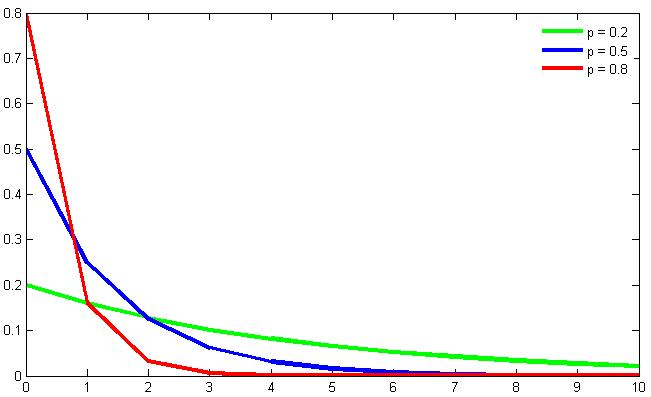
\includegraphics[width=0.7\linewidth]{Dissertation/pics/geom_distr}
    \caption{Плотность геометрического распределения при разных значениях}
  \end{minipage}
  \label{img:geom_distr}
\end{figure}

\begin{figure}[ht]
  \begin{minipage}[ht]{1.0\linewidth}\centering
    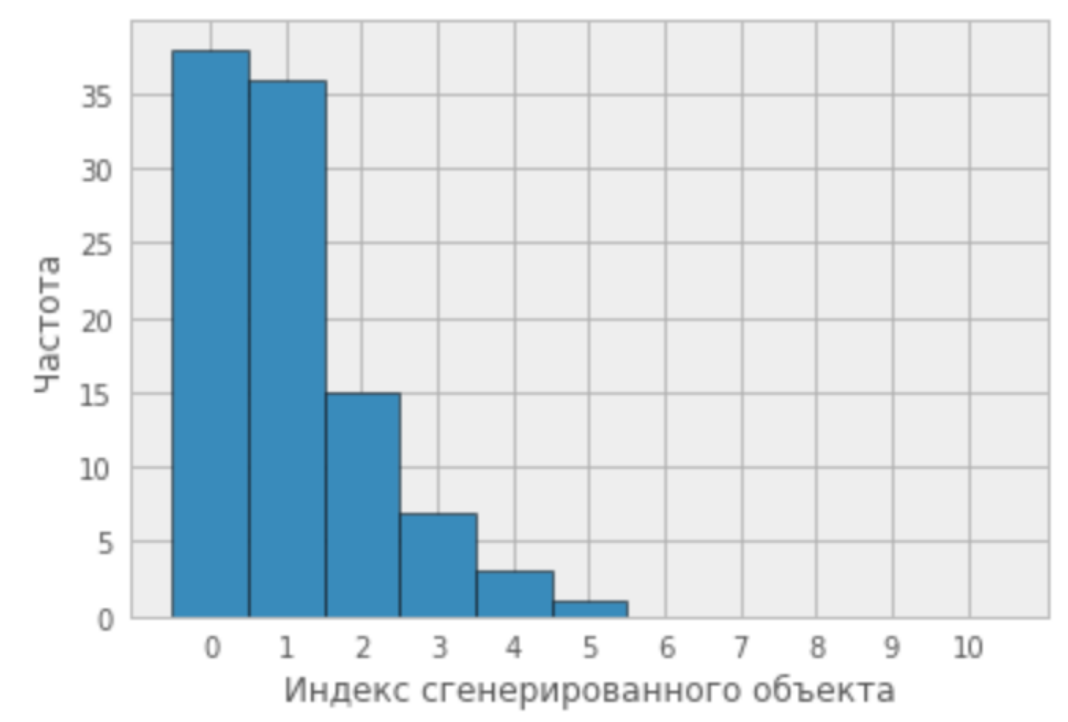
\includegraphics[width=0.7\linewidth]{Dissertation/pics/geom_distr_2}
    \caption{Зависимость количества объектов от сгенерированного индекса}
  \end{minipage}
  \label{img:geom_distr_2}
\end{figure}
После того, как положительные примеры обучающей выборки собраны, необходимо создать также и отрицательные примеры. Для отрицательных примеров используется следующий алгоритм:
\begin{enumerate}
    \item построение графа ключевых слов $\hat{G}$ по модифицированному множеству ключевых слов;
    \item для каждого слова $w$, попавшего в множество пар положительных примеров, рассматриваются случайные $k$ соседей $v_1, v_2, ..., v_k$ на расстоянии $2$ в графе $\hat{G}$;
    \item все пары $(w, v_i)_{i=1}^k$ принимаются отрицательными примерами.
\end{enumerate}

\hl{Мотивация данного алгоритма в следующем. Для обучения модели отрицательные примеры должны быть содержательными: если рассматреть случайные пары ключевых слов без каких-либо дополнительных условий, то большинство полученных примеров не будут представлять особой значимости для модели, потому что большинство статистических характеристик будут нулевыми или слишком малыми (между случайными вершинами в графе может не быть путей, они могут не иметь общих соседей, могут быть расположены на слишком большом удалении друг от друга и т.д.). Очень вероятно, что такие абсолютно случайные пары действительно не имеют и модель действительно легко научится различать положительные и отрицательные экземпляры выборки. Однако,  это не дает никакой информации для модели для более сложных случаев, когда слова находятся достаточно близко друг к другу в графе и имеют достаточну большую вероятность быть похожими. И именно такие случаи и представляют интерес в рамках данной задачи.}

\hl{С другой стороны, если для вершины в качестве отрицательных примеров брать непосредственных соседей в графе (то есть максимально близкие вершины), то слишком часто будут появляться пары, которые в действительности близки по смыслу. Это происходит потому, что среди слов одного набора могут встречаться похожие слова. В следствии этого, среди отрицательных примеров будет большое число false-negative примеров (то есть примеров, которые ошибочно были промаркированы отрицательными), что не позволит качественно обучить модель.}

\hl{Поэтому соседи вершины на расстоянии $2$ видятся наиболее подходящим компромиссом: среди них не так часто встречаются семантически близкие пары, но при этом они несут в себе содержательный сигнал, на котором можно эффективно обучаться.}
\subsubsection{Окончательная версия алгоритма}

\begin{itemize}
    \item Входные параметры: $N$, $p$, $k$;
    \item для каждого набора ключевых слов $W \in W_X$ системы $X$:
        \begin{itemize}
            \item для каждого \textit{вхождения} ключевого слова $w$:
                \begin{itemize}
                    \item если количество вхождений в коллекцию превосходит пороговое значение $N$:
                        \begin{itemize}
                            \item из геометрического распределения с параметром $p$ выбирается число;
                            \item вхождение ключевого слова $w$ заменяется $w@p$;
                            \item слово $w@p$ заносится в список модификация для слова $w$;
                        \end{itemize}
                    \item иначе
                        \begin{itemize}
                            \item вхождение ключевого слова $w$ заменяется $w@0$;
                        \end{itemize}
                \end{itemize}
            \item модифицированная версия набора ключевых слов добавляется в множество $W^{*}_X$
        \end{itemize}
    \item для каждого уникального ключевого слова $w$
        \begin{itemize}
            \item каждую пару модификаций $(w@i, w@j)$ ключевого слова $w$ добавить в обучающее множество $X_{train}$ в качестве положительного примера;
        \end{itemize}
    \item для модифицированной версии коллекции наборов ключевых слов $W^{*}_X$ добавить произвести построение графа ключевых слов $G^{*}$;
    \item для каждой вершины $w@i$ из множества модифицированных вершин графа $G^{*}$:
        \begin{itemize}
            \item выделить множество  $G_{2}(w@i) = neigbors(G^{*}, w@i, 2)$ соседей вершины $w@i$ в графе $G^{*}$ на расстоянии $2$
            \item из множества $G_{2}(w@i)$ выбрать случайно $k$ вершин $v_1, ... v_k$ и для каждой вершины добавить пару $(w@i, v_j)$ в $X_{train}$ в качестве отрицательного примера.
        \end{itemize}
\end{itemize}

Значения параметров $N$, $p$, $k$ были определены как $10$, $0.9$, $5$ соответственно.

Вхождением ключевого слова в описанном выше алгоритме является появление ключевого слова в одном конкретном наборе ключевых слов. Поскольку одно слово может присутствовать во многих наборах, то число вхождений равно количеству наборов, содержащих данное ключевое слово.


\textbf{Утверждение 3.} Расчет искусственной обучающей выборки имеет сложность $O(f^2 * k + w^2 * k^2)$, где $f$ - максимальная частотность слова в коллекции, $k$ - количество уникальных слов в коллекции, $w$ - максимальный размер набора в коллекции ключевых слов.

%Процедура $m$ - максималь
%кол-во уникальных k
%кол-во наборов m
%максимальное число слов в наборе w
%максимальная частотность слова в коллекции f
%w * m - прошли по наборам, модиф кл слова.
%
%f * k - все наборы, один раз прошлись
%f^2 - модификаций для одного слова
%f^2 * k - для всех
%f * k - построение графа
%k - максимальный размер набора (все уникальные слова попали в один набор)
%k * k  (http://www.cs.tau.ac.il/~zwick/papers/sparse.pdf умножение matr n*n -> m*n , m=nnz)
% http://www.stat.ucdavis.edu/~chohsieh/teaching/ECS289G_Fall2015/complexity.pdf
%f^2 * k + k^2

\textbf{Лемма 1.} Расчет положительных примеров искусственной обучающей выборки имеет сложность $O(f^2 * k)$, где $f$ - максимальная частотность слова в коллекции, $k$ - количество уникальных слов в коллекции.

\textbf{Доказательство.} 
Число всех ключевых слов системы с повторениями не превышает значение $f * k$. Необходимо пройти один раз по всем ключевым словам коллекции, чтобы сгенерировать для них модифицированную версию - это требует $O(f * k)$ времени. При этом полагается, что выбор случайного числа из выбранного распределения занимает константное время. Следующим шагом необходимо из модифицированных версий каждого слова получить всевозможные пары. Для каждого из $k$ слов может быть получено не более, чем $f$ модификаций слова, поскольку каждая модификация была получена из некоторого исходного слова, которое в свою очередь было использовано не более, чем $f$ раз в коллекции. Для генерации всех пар для данного исходного слова необходимо $O(f^2)$ времени, а для всех уникальных слов - $O(k * f^2)$.

\textbf{Лемма 2.} Расчет отрицательных примеров искусственной обучающей выборки имеет сложность $O(w^2 * k^2)$, $k$ - количество уникальных слов в коллекции, $w$ - максимальный размер набора в коллекции ключевых слов.

\textbf{Доказательство.} 
. Построение графа ключевых слов занимает не более $O(k^2)$ времени. Далее необходимо рассчитать соседей для каждой вершины на расстоянии $2$. Для этого необходимо возвести в квадрат матрицу смежности графа. При хранении графа в виде разреженной матрицы, операция умножения матрицы размера $(k*k)$ на себя требует $O(nnz * k)$ операций, где $nnz$ - количество ненулевых элементов. Поскольку в графе ключевых слов ребрами являются те пары ключевых слов, которые входят в один набор, то количество ребер в графе, как и количество ненулевых элементов в матрице смежности, не превышает $O(w^2 * k)$, то сложность поиска соседей второго порядка будет равна $O(w^2 * k^2)$. Предполагая, что операция взятия случайного числа занимает константное время, получаем, что генерация отрицательных примеров для искусственной обучающей выборке требует $O(w^2 * k^2)$ операций.

Из двух доказанных выше лемм немедленно следует утверждение 3.

%\begin{Алгоритмо
\subsection{Признаковое описание модели машинного обучения}
...
\subsection{Описание и настройка модели машинного обучения}
...

\subsection{Тестовые испытания}
...
\section{Построение тезауруса ключевых слов по коллекции наборов}
...
\subsection{Алгоритм построения}
...
\subsection{Тестовые испытания}
...
\section{Методы кластеризации ключевых слов по графам ключевых слов}
...
\section{Выводы}

\chapter{Определение смысловой близости пары наборов ключевых слов} \label{chapt_tuple_similarity}

% SYNOPSIS_3 >>>
В настоящей главе представлены разработанные автором настоящей работы модели и алгоритмы, позволяющие  определять уровень смысловой близости между двумя наборами ключевых слов.  С помощью таких алгоритмов можно определять уровень близости пары объектов информационно-аналитической системы, с которыми ассоциированы рассматриваемые наборы ключевых слов.
Семантическая близость между наборами ключевых слов определяется с использованием введенных в предыдущей главе методах определения семантической близости между парой ключевых слов.

Семантическая близость, рассматриваемая в рамках данной главы, является важной и востребованной на практике мерой. Она используется для решения различных задач информационного поиска. В качестве примеров таких задач могут выступать:
\begin{itemize}
    \item поиск экспертов информационно-аналитической системы, схожих по области интересов с заданным;
    \item определение множества статей и публикаций схожей тематики;
    \item рекомендации контента для пользователей блоговых систем и социальных сетей.
\end{itemize}

Для краткости изложения здесь и далее под наборами будут пониматься наборы ключевых слов.

% <<< SYNOPSIS_3
Первый раздел настоящей главы посвящается введению разработанной автором модели семантической близости наборов ключевых слов. В следующих за ним разделах \ref{kokoito_rozdel_pro_ologoritm} и \ref{kokoito_drugoi_rozdel} приводится описание алгоритма, представляющего такую модель, а также оптимизационные улучшения для сокращения времени работы программной реализации алгоритма. Наличие таких оптимизаций связано с необходимостью многочисленных вызовов функции определения семантической близости пары слов. В свою очередь, каждый такой вызов является достаточно сложной вычислительной операцией.

В заключительной части главы представлены результаты тестовых испытаний программных реализаций алгоритмов, сформулированы выводы по результатам выполненной работы, а также идеи по дальнейшему улучшению качества определения семантической близости наборов ключевых слов.

\section{Модель определения смысловой близости наборов ключевых слов} \label{tuple_model}

% >>> SYNOPSIS_3.1
Решаемая задача имеет следующую постановку. Дано множество $D$ объектов (текстовых, графических, видео документов или физических объектов другой природы) и  множество ключевых слов $W$. Каждый элемент $d_i \in D$ представлен конечным набором из $k_i$ ассоциированных с ним ключевых слов из множества $W: d_i = (w_{i,1},w_{i,2},...,w_{i,ki})$. 

Необходимо разработать такую функцию близости $TupleSim : 2^W \times 2^W \rightarrow [0, 1]$, высокие значения которой означали бы высокий уровень смысловой близости между наборами и, следовательно, соответствующими объектами системы. 

К разрабатываемой метрике близости предъявляются следующие требования.
\begin{itemize}
    \item Программная реализация должна быть способна вычислять значения метрики в режиме реального времени. Значительные задержки между отправленным пользователем запросом и полученным ответом не могут быть слишком долгими, иначе использование такой системы будет трудновыполнимым или неэффективным.
    \item Необходимо уметь вычислять уровень близости, в том числе, и для тех наборов, слова которых не представлены в системе. Существенная доля поисковых запросов содержит слова, которые ранее не были заданы ни разу и, что более важно, не встречаются в описаниях к объектам системы.
\end{itemize}


Основой для модели определения уровня близости являются модели определения семантической близости пары ключевых слов, описанные в предыдущей главе. В качестве базовых  блоков определения близости наборов ключевых слов естественно положить идеи о близости между словами, из которых состоят эти наборы. Формально, согласно принятым в гл.\ref{chapt_word_similarity} определениям, это можно описать как $TupleSim(d_i, d_j) = TupleSim(WordSim(w_{i,1}, w_{j,1}), ... , WordSim(w_{i,ki}, w_{j,kj}))$.

Для вычисления уровня близости используется простое эвристическое соображение. Суть его заключается в следующем. Два набора $d_i$ и $d_j$ обладают большим значением семантической близости, если каждому из слов набора $d_i$ можно сопоставить хотя бы одно семантически близкое слово из набора $d_j$. Таким образом, исследуемая модель в значительной мере опирается на пословные модели, описанные в предыдущей главе, перенимая как их достоинства, так и недостатки.

Преимущество такой модели заключается в эффективном использовании информации, пришедшей от моделей пословного уровня. Они, как было описано в гл.\ref{chapt_word_similarity}, демонстрируют хороший уровень качества даже в условиях недостатка данных. Основным недостатком является время вычисления меры близости между наборами в рамках такой модели. Причина заключается в том, что расчет уровня пословной близости является трудоемкой задачей. Рассматриваемая модель, в свою очередь, подразумевает многократные вызовы фукнции пословной близости.

В следующих далее разделах \ref{kokoito_rozdel_pro_ologoritm} и \ref{kokoito_drugoi_rozdel} подробно описываются алгоритмы вычисления семантической близости пары наборов ключевых слов. В то время, как в разделе \ref{kokoito_rozdel_pro_ologoritm} дается описание основных шагов для вычисления семантической близости, раздел \ref{kokoito_drugoi_rozdel} представляет дополнительный набор эвристических и инженерных идей по оптимизации вычислений. Такие улучшения дают возможность вычислять меру семантической близости более эффективно.

% SYNOPSIS_3.1 >>>

%TODO что это?
%При определении функции $TupleSim$ были использованы следующие соображения:
%begin{itemize}
%   \item как правило, если ключевое слово
%end{itemize}


\section{Алгоритм определения уровня близости пары наборов, основанный на переборе всех пар ключевых слов} \label{kokoito_rozdel_pro_ologoritm}
Первая версия алгоритма определения семантической близости наборов ключевых слов представлена следующим образом.
\begin{itemize}
    \item Входные данными алгоритма является пара наборов $d_i = (w_{i,1},w_{i,2},...,w_{i,ki}), d_j = (w_{j,1},w_{j,2},...,w_{j,kj})$.
    \item Для каждой пары ключевых слов $w_{i,p}, w_{j,q}$ с индексами $p \in [1, k_i], q \in [1, k_j]$:
        \begin{itemize}
            \item вычисляется признаковые характеристики, описанные в \ref{sec:features};
            \item посчитанный массив значений передается предобученной модели XGBoost, описанной в \ref{ml_sim};
            \item происходит предсказание пословной близости моделью;
            \item результаты сохраняются в ячейке $(p, q)$ матрицы $m_{sim}$ размером $k_i, k_j$.
        \end{itemize}
    \item Из каждой строки матрицы $m_{sim}$ выбирается наибольшее значение.
    \item По этим наибольшим значениям вычисляется среднее, которое возвращается в качестве меры близости для пары рассматриваемых наборов.
\end{itemize}

Далее приведены примеры близких наборов ключевых слов, согласно описанной модели. При построении примеров рассматривались наборы, имеющие пустое пересечение по словам. Следующие далее примеры представляют существенно больший интерес.

\begin{tabularx}{16cm}{|X|X|X|}
        \hline
        Первый набор & Второй набор & Значение функции близости \\ \hline
        мультиферроики, магнитные структуры, фазовые переходы, магнитоэлектрики, сильные магнитные поля & магниторезонансная томография, гигантское комбинационное рассеяние, суперпарамагнетизм & 0.82 \\ \hline
        мембранные белки, молекулярное моделирование, фоточувствительные белки, ретиналь, молекулярная динамика, membrane proteins, molecular modeling, retinal, molecular dynamics, photosensitive proteins & малые белки теплового шока, универсальный белковый адаптер 14-3-3, фосфорилирование & 0.68 \\ \hline
        социальная теория, социальная философия, понятие общества, философия истории & идея, социальная практика, научно-технический прогресс, наука, парадигма & 0.57 \\ \hline
        мультиферроики, низкоразмерные и фрустрированные магнитные системы, термодинамические и резонансные свойства, зарядовое и орбитальное упорядочение & магниторезонансная томография, гигантское комбинационное рассеяние, суперпарамагнетизм & 0.8 \\ \hline

\end{tabularx}

Пары наборов ключевых слов, имеющие в своем составе общие слова, представляют существенно меньший интерес, чем пословно различные пары. Причина заключается в том, что определение высокого уровня близости для наборов, имеющих в составе одинаковые слова, является простой задачей. Другими словами, факт наличия общего слова в паре наборов в значительной мере повышает уровень семантической близости. Для определения близости в случае повторяющихся слов можно воспользоваться, например, описанной ранее мерой Жаккара. Напротив, сложной задачей является построение модели, способной определять уровень семантической близости для различающихся пословно наборов.

Представленные выше примеры демонстрируют способность предлагаемой модели выявлять близость между наборами, не имеющими общих слов, что свидетельствует о ее практической ценности. Отмечается, однако, что такой алгоритм не является вычислительно эффективным. Такая его реализация не позволит вычислять уровень близости для большого числа пар наборов. Этот факт, в свою очередь, ставит под сомнение возможность использования программное реализации в существующих информационно-аналитических системах. Способы преодоления описанных выше трудностей представлены в следующем разделе.

\section{Оптимизированный алгоритм определения близости пары наборов} \label{kokoito_drugoi_rozdel}

Описанный в разделе \ref{kokoito_rozdel_pro_ologoritm} алгоритм определения уровня близости пары наборов ключевых слов с полным перебором всех пар ключевых слов по экспертной оценке имеет достаточно высокий уровень качества. Однако, он имеет и существенный недостаток. Этот недостаток заключается в низком уровне быстродействия его программной реализации. 

Существует несколько составляющих алгоритма, которые главным образом влияют на скорость вычисления уровня близости. Первый из них заключается в рассчете попарных уровней близости между словами разных наборов. Эта процедура имеет асимптотическую сложность $O(mn)$, где $m$, $n$ - размеры наборов. Таким образом, для пары наборов необходимо рассчитать 30-50 уровней близости между словами этих наборов.

Отметим, что значение рассчитанных значений функций близости можно сохранять и переиспользовать. В предствленной выше наивной версии алгоритм опирается на факт необходимости вычисления уровней близостей для всех возможных пар. Однако, представляется логичным следующее предположение: если для слова из первого набора уже найдено близкое слово из второго, то нет необходимости продолжать сравнивать это слово с другими словами второго набора. Например, если в одном наборе присутствует слово <<белок>>, а в другом слово <<протеин>>, то установив факт близости, можно остановиться и не вычислять близость слова <<белок>> до других слов другого набора (<<мембранные белки>>, <<молекулярное моделирование>>, <<фоточувствительные белки>>, <<ретиналь>>).

Следующим узким местом с точки зрения вычислительной производительности является непосредственно вычисление значений функции близости, которая определена в главе \ref{chapt_word_similarity}. Для вычисления уровня близости необходимо применить обученную модель из раздела \ref{ml_sim}. В наивном варианте алгоритма, описанного в предыдущем разделе, функция применения модели выполняется для каждой пары рассматриваемых слов. Однако, более эффективным является применение модели сразу для всего множества рассматриваемых пар.

На более низком уровне сложность вычисления зависит от скорости вычисления признаков для пары ключевых слов, описанных в \ref{sec:features}. Естественно, что все необходимые графы хранятся в оперативной памяти, их загрузка и построение происходит один раз до вычисления значений функций уровня близости. При этом вычисления различных графовых характеристик (таких как длины путей, степени абстрактностей вершин и другие) выполняются каждый раз для каждой пары ключевых слов. Это значительно замедляет вычислительный процесс. Поэтому была проведена оптимизация вычисления признаков, которая будет описана далее. Исходя из соображений, описанных выше, алгоритм был оптимизирован при помощи следующих перечисленных далее действий.
\begin{itemize}
    \item В качестве значения близости между одинаковыми словами $WordSim(w, w)$ автоматически ставится уровень близости 1. Как было показано в разделе \ref{sec:test_equal}, с помощью модели вычисления близости пары слов можно правильно определять наивысший уровень близости между тождественно равных слов. Поэтому в целях оптимизации необходимо избегать вызовов функций от одинаковых слов и в этом случае за уровень близости принимать максимально возможное значение.
    \item Если для слова уже найдено похожее к нему по уровню близости, то вычисления близости до других слов не происходит. Процесс вычисления останавливается, если для данного слова найдено близкое по смыслу слово в другом наборе и уровень близости превышает значение 0.4.
    \item Выполнение предрассчета значений близости для самых частотных пар ключевых слов. Вычислив заранее необходимые уровни близости для пар самых популярных в системе ключевых слов, можно добиться ускорения вычисления значений функции близости пары наборов ключевых слов.
    \item Выполнение предрасчета значений некоторых признаков модели машинного обучения. 
    \item Применение модели машинного обучения в момент, когда все признаки для всех необходимых пар посчитаны. Это позволяет оптимально использовать матричные операции при вычислении значений формулы.
\end{itemize}

Данные средства позволяют значительно уменьшить среднее время выполнения вычисления близости. Тестированию производительности, а также качества определения близости программной реализации представленного выше алгоритма посвящен раздел \ref{tuple_test}. 

\section{Тестовые испытания} \label{tuple_test}
В качестве примера, который, с одной стороны, иллюстрирует практическую востребованность представленного алгоритма в информационно-аналитических системах, а с другой, показывает его работоспобоность, рассмотрим тестовые данные, содержащиеся в ИАС <<ИСТИНА>>.
Для проведения тестовых испытаний программных реализаций функции определения близости наборов ключевых слов были взяты данные о научных проектах в МГУ, аккумулированные в ИАС <<ИСТИНА>>. Этот набор данных содержит в себе информацию о выполненных и занесенных в систему научных проектах, а также следующую сопутствующую информацию:
\begin{itemize}
    \item название проекта;
    \item название проекта на английском языке (может отсутствовать).
    \item идентификационный номер проекта;
    \item короткое текстовое описание проекта (может отсуствовать);
    \item набор ключевых слов (может отсутствовать);
    \item руководители участники проекта (заданы идентификационными номерами, может отстутствовать);
    \item факультет, институт которого выполняет проект (задан идентификационными номерами, может отсутствовать).
\end{itemize}

Всего в наборе данных присутствует информация о $12350$ проектах.

Для тестирования программной реализации моделей определения уровня близости было проведено два эксперимента над рассмотренным набором данных. Кроме этого, в ходе экспериментов было проведено измерение производительности реализаций моделей. Рассмотренная в настоящей главе модель определения близости наборов сравнивается с классической мерой близости Жаккара для наборов и моделью Word2Vec, обученной на большом объеме (12.9 млрд. словоупотреблений) данных в рамках проекта Russian Distributional Thesaurus. Близость наборов с помощью модельи Word2Vec вычислялась по следующему алгоритму:
\begin{itemize}
    \item для каждого слова каждого набора рассматривались его векторные представления моделью;
    \item векторное представление набора определяется как среднее по векторам входящим в него слов;
    \item вычисляется косинусное расстояние между векторами наборов - оно возвращается в качестве близости наборов ключевых слов.
\end{itemize}
        
Далее описывается процедура каждого из экспериментов и приводятся результаты тестирования. 

\textbf{Тестирование близости научных проектов по факультетам.} Тестирование качества разработанного алгоритма близости проведено с использованием имеющихся данных о выполняемых в вузах и НИИ научных проектах на примере МГУ и основывается на следующей идее.
Естественно предположить, что  внутри одного факультета, проекты не так сильно отличаются друг от друга и, следовательно, ключевые слова проектов одного факультета должны быть в среднем более похожи друг на друга, чем слова разных факультетов. Исходя из этих рассуждений, был подготовлен тестовый набор данных. В качестве примеров близких по смыслу наборов ключевых были взяты пары наборов, проекты которых принадлежат одному факультету. Для каждого набора $W$, для которого определены положительные примеры $\overline{W}_{1}, ... \overline{W}_{k}$, случайным образом из множества проектов других факультетов выбирается 1000 проектов. Наборы $\hat{W_1}, ..., \hat{W}_{1000}$, соответсвующие этим проектам, объявляются семантически непохожими на набор $W$. Таким образом, для набора $W$ присутствует $k$ наборов, объявленных похожими по смыслу к $W$, и $1000$ наборов, объявленных непохожими.

Далее для каждого набора $W$ моделями $TupleSim$, $Word2Vec$ и  $Jaccard$ вычисляются меры близости. Но основе правильных ответов и ответов, определенных моделями, для каждого из подходов подсчитывается метрика $ROC-AUC$. Значение этой метрики усредняется по всем $W$.

Результаты тестирования приведены в следующей далее таблице \ref{tbl:tuple_test}.

Отмечается, что абсолютные значения в данном эксперименте не играют существенной роли: набрать стопроцентный результат и даже близкий к нему не представляется возможным в силу построения тестирущего множества. Дело в том, что в действительности проекты одного факультета не обязаны быть строго похожими друг на друга. Напротив, многие из них могут сильно различаться, но согласно эксперименту, в этом случае они все равно будут объявлены как близкие и если модели факт близости не установят, то значение метрики уменьшится. 

Однако, связь между близостью наборов и принадлежностью их к одному факультету присутствует. Разработанная автором настоящей диссертации модель лучше других известных моделей установила эту связь, что является показателем ее качества. Этому факту свидетельствуют результаты тестовых испытаний, приведенные в таблице \ref{tbl:tuple_test}.

\textbf{Тестирование наборов с общими словами.}
В качестве дополнительного способа проверки качества было проведено следующее исследование. Как и прежде, в качестве входных данных выступает информация о научных проектах в МГУ, аккумулированная в ИАС <<ИСТИНА>>. Данный эксперимент аналогичен предыдущему, но вместо факта принадлежности пары проектов одному факультету используется факт существования общего ключевого слова у ключевых наборов двух проектов. Предполагается, что вероятность семантической близости пары наборов, имеющих общее слово, выше, чем случайной пары наборов. Более сильное предположение, что даже если удалить это общее слово, все равно близость между такими наборами должна быть в среднем выше, чем у случайных.

Множества $\overline{W}_{1}, ... \overline{W}_{k}$ и $\hat{W_1}, ..., \hat{W}_{1000}$ собирались таким же способом, как в предыдущем эксперименте. Результаты тестовых испытаний приведены в таблице \ref{tbl:tuple_test}

Отмечается, что и в этом испытании разработанная автором модель показала лучший результат. Важно также отметить, что модель $Jaccard$ отстает более значительно от двух других. Причиной этому является то, что удаление общего слова в рассматриваемых парах в подавляющем большинстве случаев (порядка 80\%) означает, что больше общих слов в наборах не осталось. По определению меры, близость для таких наборов будет равна нулю. А это значит, что у таких примеров нет возможности сделать метрику качества выше 0.5.

\textbf{Тестирование производительности программной реализации модели близости.}
Для тестирования производительности программной реализации модели близости наборов ключевых слов был проведен эксперимент. Необходимость этого эксперимента обусловлена тем фактом, что исследуемая функция близости должна обладать достаточным уровнем быстродействия для возможности ее использования в реальных системах. Для тестирования было измерено время расчета функции близости для трех моделей на обоих качественных экспериментах, описание которых приводится ранее в настоящем разделе. Результаты также приведены в таблице \ref{tbl:tuple_test}.

\begin{table}[H]
\begin{tabularx}{16cm}{|X|X|X|X|} 
        \hline
        Модель & Тип тестирования & Метрика ROC-AUC &  Время расчета в сек. \\ \hline
        Jaccard & Факультеты &0.564 & 8 \\ \hline
        Word2Vec & Факультеты &0.672 & 12 \\ \hline
        \textbf{TupleSim} & Факультеты & \textbf{0.692} & 15 \\ \hline
        Jaccard & Общее слово & 0.601 & 3 \\ \hline
        Word2Vec & Общее слово & 0.720 & 4 \\ \hline
        \textbf{TupleSim} & Общее слово& \textbf{0.764} & 8 \\ \hline
\end{tabularx}
\caption{Результаты тестирования} \label{tbl:tuple_test}
\end{table}
Тип тестирования <<Факультеты>> соответствует тестированию близости научных проектов по факультетам. В свою очередь, тип <<Общее слово>> обозначает тестирование наборов с общими словами. По метрике ROC-AUC разработанная автором модель превосходит известные модели определения близости в рамках рассмотренных экспериментов.

Следует отметить, что модель $Word2Vec$ обучена на огромных объемах данных. Время обучения такой модели требует недель или месяцев процессорного времени. Однако это дает возможность более эффективно использовать обученные векторные представления и быстро вычислять функцию близости. Модель $Jaccard$ способна вычислять степень близости более быстро за счет своей простоты. Несмотря на это, разработанная автором модель $TupleSim$ показывает лучшее качество, с относительно небольшим отставанием по времени.

\section{Выводы}
По результатам исследований, проведенных в рамках настоящей главы, были разработаны модели определения уровня семантической близости пары наборов ключевых слов. Для построения таких моделей используются пословные модели семантической близости, подробно описанные в гл.\ref{chapt_word_similarity}. Для разработанных моделей представлены алгоритмы и программные реализации этих алгоритмов. Тестовые испытания, проведенные в разделе \ref{tuple_test}, демонстрируют улучшения качества определения уровня семантической близости в сравнении с известными моделями.

Следующим шагом в исследованиях может стать разработка модели представления набора ключевых слов. Суть такого представления заключается в следующем. По аналогии с идеями, заложенными авторами \cite{word2vec} в модель \emph{Word2Vec}, представляется возможность построить векторное представление для каждого набора ключевых слов системы. Близость пары таких векторов будет означать близость соответствующих им наборов ключевых слов.

Существующие модели построения представлений обучаются на данных широкого профиля, что не позволяет передать специфику рассматриваемой интеллектуально-аналитической системы. Другой подход, заключающийся в обучении таких моделей на имеющихся в системе данных, не способен показать высокий уровень качества, если система не обладает большими объемами накопленной информации. По этим причинам важным в построении новой модели представлений является использование пословных моделей близости, описанных в гл.\ref{chapt_word_similarity}. Как и модели, описанные в настоящей главе, новые модели смогут обучаться на небольших объемах данных, эффективно используя модели близости пары слов. В то же время, процесс вычисления семантической близости сведется в этом случае  к прозрачной и вычислительно эффективной процедуре определения близости пары векторов. Такой подход полностью разрешит вопрос долгого вычисления функции близости наборов ключевых слов.

%\section{Алгоритмы определения смысловой близости коротких предложений}
%\section{Методы кластеризации наборов ключевых слов}
%\begin{table} [htbp]% Пример записи таблицы с номером, но без отображаемого наименования
%	\centering
%	\parbox{18cm}{% чтобы лучше смотрелось, подбирается самостоятельно
%        \captiondelim{}% должен стоять до самого пустого caption
%        \caption{}%
%        \label{tbl:test1}%
%        \begin{SingleSpace}
%    	\begin{tabular}{ | c | c |}
%    	\hline
%    	выпуклое программирование, принцип лагранжа, \\
%        теорема куна-таккера в недифференциальной форме, \\
%        параметрическая задача, \\
%        минимизирующая последовательность, двойственность\\
%        , регуляризация & оптимальное \\ управление \\ \hline
%    	\end{tabular}%
%    	\end{SingleSpace}
%	}
%\end{table}

%\section{Решение задачи поиска экспертов} \label{expert_search_tuplesim}
%\subsection{Определение близости наборов для решения задачи поиска экспертов}
%В качестве меры близости пары наборов ключевых слов автором предлагается следующая формула:
%$$ TupleSim_{expert}(X,Y) = \frac{\sum_{i=1}^{|X|}\sum_{j=1}^{|Y|}WordSim_{expert}(X_i, Y_j)}{|X \bigcup Y|}, $$
%
%где $|\cdot|$ ­ количество слов в наборе, $X_i$, $Y_j$ ­ $i$­ое и $j$­ое ключевые слова наборов $X$, $Y$ соответственно. $WordSim_{expert}$ - мера близости, введенная в \ref{expert_search_wordsim}. Числитель этой формулы аккумулирует близость всех пар слов из разных наборов. Если положить $WordSim_{expert}(x, y) = \mathbbm{1}x=y$, то числитель будет равен числу общих ключевых слов, что приведет к более простой модели вычисления близости по мере Жаккара. Без нормировки длинные пары наборов были бы сильнее похожи друг на друга, чем короткие пары.
%
%\section{Выводы}
%...

\chapter{Приложения моделей близости ключевых слов} \label{chapt_applications}
В настоящем разделе рассматриваются реальные задачи и системы, в которых применяются программные реализации алгоритмов. 
Рассматривается задача поиска эксперта в области, определяемой заданным запросом из ключевых слов.
Также описывается использование тезауруса ключевых слов для задачи улучшения ранжирования в поисковой составляющей интеллектуальной системы <<ИСТИНА>>.
В конце раздела представлены выводы, а также дальнейшее направление в применении разработанных программных комплексов в реальных приложениях.

\section{Решение задачи поиска экспертов} \label{expert_search}
\subsection{Постановка задачи}
Дано множество наборов ключевых слов $W_X$ и объектов информационной системы $X$, а также множество $Q$ запросов к системе. Обозначим за $W$ множество всех уникальных ключевых слов из всех наборов $W_X$. Каждый элемент $x_i \in X$ множества объектов ассоциирован с набором ключевых слов $W_i = \{w_{i_0}, w_{i_1}, ..., w_{i_{n_i}} \} \in W_X \in 2^W$. Точно также каждый запрос $q_j \in Q$ связан с некоторым набором ключевых слов $W_j = \{w_{j_0}, w_{j_1}, ..., w_{j_{n_j}} \} \in 2^W$. Необходимо определить меру близости пары запрос­объект для каждого объекта и каждого запроса, т.е.  функцию $f : Q \times X \rightarrow R$. Поскольку запросам и объектам единственным образом сопоставляются наборы ключевых слов, то задача сводится к определению меры близости на наборах: $f_w : 2^W \times 2^W \rightarrow R$. Кроме того, необходимо разработать эффективный алгоритм, который, используя меру близости и некоторые дополнительные идеи, мог бы по запросу выдавать множество объектов, наиболее релевантных данному запросу.
\subsection{Процедура поиска экспертов}
По данному множеству наборов ключевых слов (множеству экспертов) строится граф ключевых слов. Далее необходимо для каждого ключевого слова $x$ найти ближайшие по смыслу слова. Мера близости слов вычисляется сначала между тегом $x$ и его соседями в графе, после чего просматриваются соседи соседей $x$ и так до тех пор, пока не наберется фиксированное число кандидат. Часть наиболее релевантных тегов сохраняются, как наиболее близкие к $x$. В дополнение к этому, строится инвертированный индекс, который позволяет по слову восстановить наборы, содержащие это слово. После того, как в систему приходит запрос, для каждого слова из запроса выгружаются ближайшие по смыслу слова и первоначальный запрос расширяется. Затем по словам из расширенного запроса восстанавливаются наборы­кандидаты. Для каждого из них считается мера близости с исходным запросом $TupleSim_{expert}$, подробно описанная в \ref{expert_search_tuplesim}. В конце своей работы алгоритм возвращает наиболее релевантные наборы­кандидаты.
\section{Реализация поиска по ключевым словам на базе собранного тезауруса синонимов}
Программные механизмы использования ключевых слов позволяют существенно улучшить поиск необходимой пользователю информации в системе. Информацию о большинстве объектов системы (публикации, конференции, сведения о пользователях и др.) можно дополнить произвольным набором ключевых на естественном языке. После внесения информации, происходит индексирование и обработка ключевых слов, что позволяет проводить дальнейший интеллектуальный анализ данных с целью получения релевантного ответа на запрос.

Основные задачи, которые могут быть решены при помощи ключевых слов - улучшение качества поисковых алгоритмов ранжирования подлежащих анализу объектов, а также поисковые подсказки рекомендательного характера для пользователя.

Для решения обозначенных выше задач был реализован поисковый модуль на базе фреймворка Django. Он представляет собой поисковую строку, в которую вводятся ключевые слова, разделенные запятой, а также таблицы поисковой выдачи, в которой указаны объекты, удовлетворяющие критериям поиска, в порядке убывания релевантности. В момент ввода пользователю предлагается расширить свой запрос некоторыми связанными ключевыми словами, что впоследствии помогает найти более релевантные запросу объекты. Интерфейс системы представлен на рис.\ref{img:search}

\begin{figure}[ht]
  \begin{minipage}[ht]{1.0\linewidth}\centering
    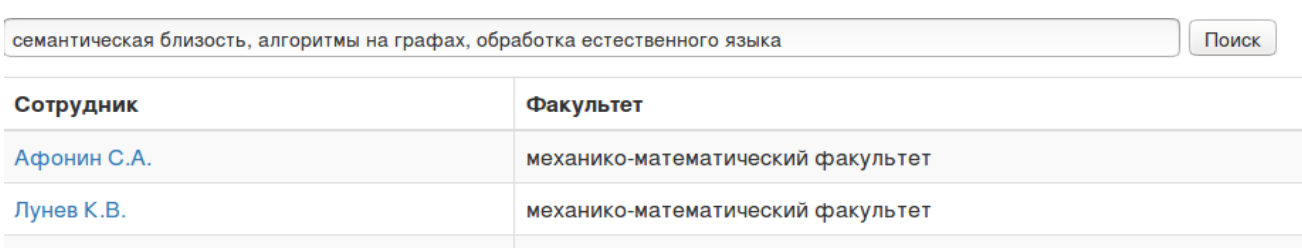
\includegraphics[width=0.95\linewidth]{Dissertation/pics/search}
    \caption{Интерфейс модуля поиска по ключевым словам}
  \end{minipage}
  \label{img:search}
\end{figure}

Помимо этого реализовано ядро подсистемы обработки ключевых слов, которое проводит основной анализ, определение семантической близости пары слов, подготовку тезауруса ключевых слов. Методы определения сематнической близости пары ключевых слов описаны в главе \ref{chapt_word_similarity}, а описание алгоритма построения тезауруса дано в разделе \ref{thes}. Код ядра представляет собой модули, процедуры и скрипты на языке Python с использованием открытых математических пакетов (Numpy, Pandas, Scipy), а также пакетов для анализа данных и машинного обучения (Scikit-learn, XGBoost). Данный модуль может использоваться отдельно от основного кода системы.

\begin{figure}[ht]
  \begin{minipage}[ht]{1.0\linewidth}\centering
    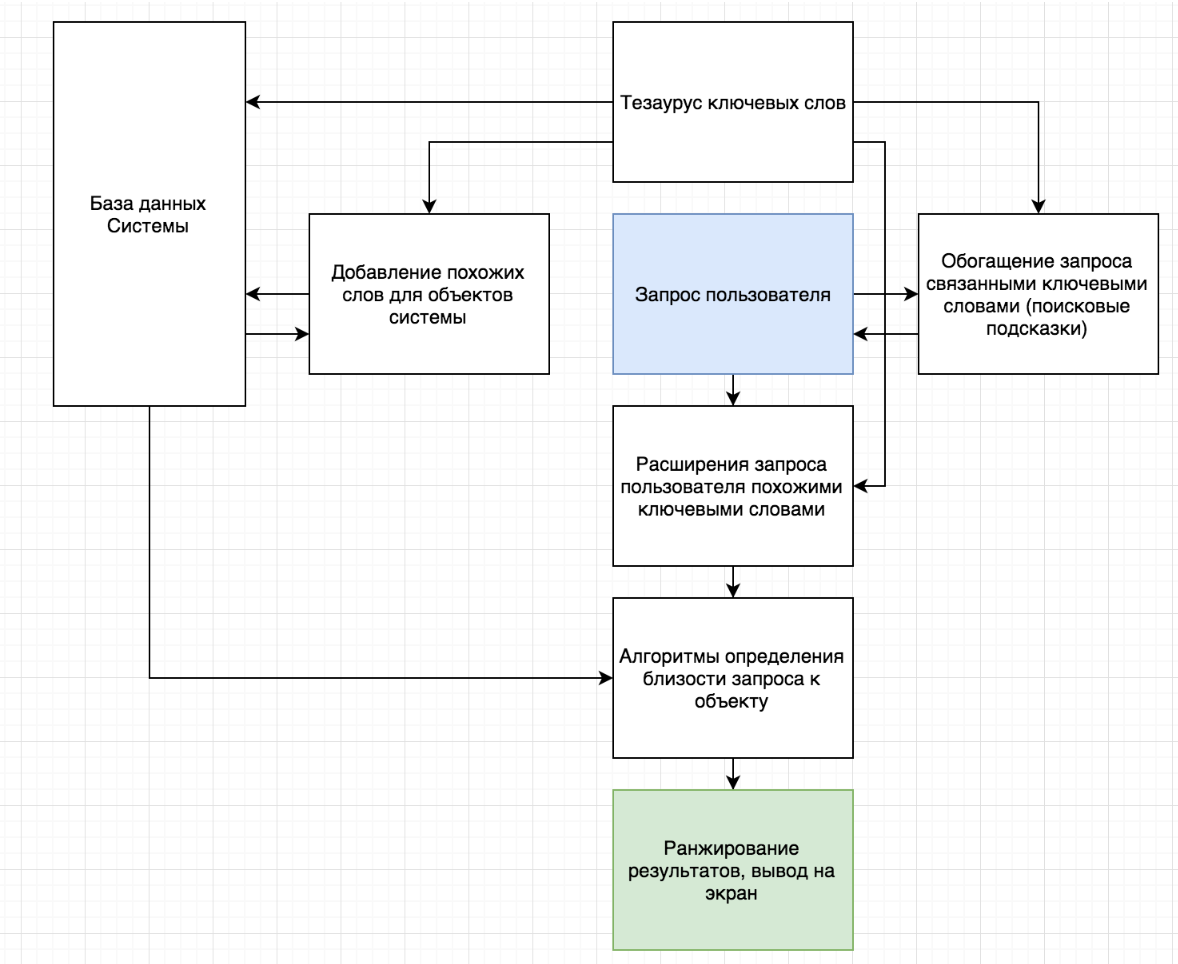
\includegraphics[width=0.95\linewidth]{Dissertation/pics/search_2}
    \caption{Схема обработки запроса на поиск по ключевым словам}
  \end{minipage}
  \label{img:search_2}
\end{figure}

На рис.\ref{img:search_2} представлена схема выполнения и обработки запроса. Основной процесс работы с ключевыми словами состоит из трех шагов. На первом из них в ядре модели рассчитывается тезаурус ключевых слов. В этом тезаурусе для каждого ключевого слова хранятся ключевые слова, близкие по смыслу к данному, с указанием значения меры близости. Далее полученный словарь загружаются в базу данных системы, после чего появляется возможность по введенному пользователем слову быстро восстанавливать множество ключевых слов, похожих на заданное. Данный этап сбора словаря стоит обособленно от процесса поиска и может быть перезапущен в любой момент времени. 

Второй шаг - обогащение объектов системы ключевыми словами из собранного на прошлом шаге тезауруса. Если для объекта указан набор ключевых слов, то для к каждому из этих ключевых слов добавляется информация о близких словах из тезауруса. Данный этап также является шагом предобработки данных. 

Последний этап - непосредственно поиск по ключевым словам. Введенный пользователем запрос расширяется словами тезауруса, далее происходит поиск сущностей по расширенным наборам ключевых слов (как в запросе, так и в описании объекта). Для найденных объектов вычисляется релевантность (функция, возвращающая действительное число по паре запрос-объект, большие значения которой соответствуют более релевантным объектам), результаты сортируются по убыванию релевантности и выводятся на экран пользователя. Использование поискового запроса пользователя как набора ключевых слов, позволяет применять упомянутые выше алгоритмы для разработки поисковых подсказок. Такие подсказки предлагают пользователю дополнить свой запрос ключевыми словами, связанными по смыслу с теми, которые он уже ввел.

Трудностью в решении задачи реализации поиска по ключевым словам является тот факт, что для значительной части слов в системе нет достаточной статистики их использования. Как следствие, возникает ситуация, когда про слово, добавленное к описанию объекта или про слово, заданное пользователем в поисковую строку, нет достаточной информации, что не позволяет получить релевантную запросу поисковую выдачу. Для преодоления этой трудности в системе реализованы интеллектуальные алгоритмы анализа ключевых слов, а также используются внешние корпусы данных на естественном языке, описанные в разделе \ref{ml_sim}. Основными направлениями работы по использованию ключевых слов для выполнения поисковых запросов являются следующие:

\begin{itemize}
    \item определение семантической близости между парой ключевых слов с помощью алгоритмов машинного обучения и внешних наборов данных;
    \item определение семантической между парами наборов ключевых слов;
    \item использование связей между объектами системы (например, списки публикаций одного автора, таблицы соавторства, списки участников конференции, работников лаборатории и др.)
\end{itemize}

Таким образом, поиск по ключевым словам осуществляет не только определение точного вхождения слов запроса в слова объектов, по которым ведется поиск, но также происходит расширение как запроса, так и подлежащих анализу документов семантически близкими словами. В дополнении к этому, наборы ключевых слов, ассоциированные с объектами системы, обогащаются словами, от связанных с ними объектов. Все это позволяет увеличить описание к имеющимся данным и, следовательно, улучшить возможности поиска. 


\subsection{Поисковые подсказки для ключевых слов}
Поисковые подсказки позволяют облегчить пользователю формулировку запроса к системе на естественном языке. Стандартные алгоритмы построения поисковых подсказок позволяют выбрать необходимое слово по его введенному префиксу. Но во многих ситуациях является важным подсказать пользователю слово, близкое по значению к вводимому. Такое слово пользователь, возможно, не вспомнил во время ввода запроса. Алгоритм полезен также и в тех случаях, когда пользователь планировал ввести предлагаемое слово, поскольку это экономит время ввода: нет необходимости полностью вводить слово, его можно просто выбрать из списка предложенных слов.

Поэтому была реализована система поисковых подсказок, описание которой приведено далее:
\begin{itemize}
    \item известные системе ключевые слова кладутся в префиксное дерево;
    \item в листья префиксного дерева кладутся ссылки на ключевые слова, близкие к слову, построенному от вершины дерева до этого листа;
    \item при вводе пользователем слова, в интерфейсе появляется список возможных завершений данного слова, построенный обходом от текущей вершины в префиксном дереве;
    \item при достижении листовой вершины (путем полного ввода слова или выбора подсказки) в интерфейсе показывается список слов, близких по смыслу к только что введенному. Слова этого списка отсортированы по уменьшению значения функции семантической близости;
    \item при выборе одного из слов из списка семантически близких к введенному, это слово добавляется в запрос. Пользователю предлагается выбрать близкие слова к только что добавленному или начать вводить следующее слово самостоятельно.
    \item при нажатии на кнопку <<Поиск>> начинается процесс построения поисковой выдачи по введенному запросу.
\end{itemize}
        
\section{Выводы}
%\

%\include{Dissertation/part1}           % Глава 1
%\include{Dissertation/part2}           % Глава 2
%\include{Dissertation/part3}           % Глава 3
\chapter*{Заключение}						% Заголовок
\addcontentsline{toc}{chapter}{Заключение}	% Добавляем его в оглавление

%% Согласно ГОСТ Р 7.0.11-2011:
%% 5.3.3 В заключении диссертации излагают итоги выполненного исследования, рекомендации, перспективы дальнейшей разработки темы.
%% 9.2.3 В заключении автореферата диссертации излагают итоги данного исследования, рекомендации и перспективы дальнейшей разработки темы.
%% Поэтому имеет смысл сделать эту часть общей и загрузить из одного файла в автореферат и в диссертацию:

Основные результаты работы заключаются в следующем.
%% Согласно ГОСТ Р 7.0.11-2011:
%% 5.3.3 В заключении диссертации излагают итоги выполненного исследования, рекомендации, перспективы дальнейшей разработки темы.
%% 9.2.3 В заключении автореферата диссертации излагают итоги данного исследования, рекомендации и перспективы дальнейшей разработки темы.
%\begin{enumerate}
%  \item Результат 1 \ldots
%  \item Результат 2 \ldots
%  \item Результат 3 \ldots
%  \item Результат 4 \ldots
%\end{enumerate}

      % Заключение
%\include{Dissertation/acronyms}        % Список сокращений и условных обозначений
%\include{Dissertation/dictionary}      % Словарь терминов
\include{Dissertation/references}      % Список литературы
%\include{Dissertation/lists}           % Списки таблиц и изображений (иллюстративный материал)
%\input{Dissertation/appendixsetup}   % Предварительные настройки для правильного подключения Приложений
\chapter{Требования к качеству программной системы анализа ключевых слов } \label{AppendixRequirements}
Настоящее приложение содержит характеристики и показатели, определяющие требования, которые предъявляются к качеству разрабатываемого программного комплекса в соответствии со стандартом \mbox{ГОСТ Р ИСО/МЭК 9126-93}.
\section{Функциональность}
\hl{Системой должен быть поддержан следующий функционал:}
\begin{enumerate}
    \item  \hl{подготовка моделей определения семантической близости пар объектов системы по имеющимся данным:}
    \begin{enumerate}
        \item  \hl{модель семантической близости пары ключевых слов;}
        \item  \hl{модель семантической близости наборов ключевых слов;}
        \item  \hl{модель семантической близости пары сущностей системы.}
    \end{enumerate}
    \hl{Самым вычислительно сложным является построение модели близости пары ключевых слов. Каждая следующая модель обучается последовательно, поскольку в значительной степени опирается на предыдущую. Весь этап обучения является алгоритмически сложной задачей и включает в себя несколько этапов:}
        \begin{itemize}
            \item \hl{предподготовка данных;}
            \item \hl{построение необходимых графов из данных;}
            \item \hl{сбор обучающей выборки для моделей;}
            \item \hl{подсчет многочисленных графовых характеристик по графам для объектов обучающей выборки;}
            \item \hl{непосредственно обучение модели.}
        \end{itemize}
    \item \hl{быстрое обновление имеющихся и добавление новых данных в систему:}
    \begin{enumerate}
        \item \hl{добавление/модификация наборов ключевых слов;}
        \item \hl{добавление/модификация дополнительных графов, связывающих сущности системы различными отношениями.}
    \end{enumerate}
    \hl{При изменении данных системы возникает необходимость переобучения моделей близости для поддержания консистентного состояния между данными и моделями. Сложность данного пункта в том, что наивная переподготовка моделей после изменения данных может занимать продолжительное время. По этой причине возникает необходимость разработки сложных алгоритмов инкрементальной подготовки моделей, что сократит время их дообучения.}
    \item \hl{быстрая кластеризация ключевых слов системы и поиск необходимого кластера;}

    \hl{Данный процесс происходит после обучения модели близости пары ключевых слов.}
    \item \hl{быстрый поиск похожих объектов с помощью обученных моделей:}
    \begin{enumerate}
        \item \hl{поиск наиболее похожих ключевых слов к заданному;}
        \item \hl{поиск сущностей, релевантных заданному набору ключевых слов;}
        \item \hl{поиск набора ключевых слов, подходящих для заданной сущности.}
    \end{enumerate}
    \item \hl{реализация подмодулей, решающих практически значимые задачи информационного поиска в рамках аналитической системы:}
    \begin{enumerate}
        \item \hl{подмодуль поиска эксперта. Реализация функционала поиска сущностей информационной системы, релевантных поисковому запросу из ключевых слов;}
        \item \hl{подмодуль предложенных ключевых слов. Реализация функционала предложения пользователю новых ключевых слов по словам, введенным на данный момент или по имеющейся связанной информации.}
    \end{enumerate}
    \item \hl{сбор пользовательской информации в ходе взаимодействия с комплексом:}
    \begin{enumerate}
        \item \hl{подмодуль поиска эксперта. Логирование релевантных и нерелевантных по мнению пользователя результатов;}
        \item \hl{подмодуль предложенных ключевых слов. Логирование выбранных и невыбранных пользователем ключевых слов из числа предложенных.}
    \end{enumerate}
    \hl{Поиск должен выполняться как только пользователь ввел запрос и подтвердил его. Вычисление и показ результатов должны укладываться в несколько секунд. Сложность данного требования в том, что для каждого запроса необходимо подсчитать огромное число графовых характеристик и применить соответствующую предобученную графовую модель близости. В следствии этого данный пункт представляет собой сложную техническую задачу по оптимизации вычислений.}
    \item \hl{cоответствие принятым в индустрии соглашениям и стандартам;}
    \item \hl{высокий уровень доверия и защищенность ресурсов системы от деструктивных воздействий путем соблюдения положений (стандартов) информационной и функциональной безопасности, а также использования программного обеспечения с открытым исходным кодом;}
    \item \hl{система должна функционировать под управлением ОС с открытым исходным кодом.}
\end{enumerate}

\section{Надежность}
Следующие свойства должны быть удовлетворены:
\begin{enumerate}
    \item  \hl{качество обученных моделей должно валидироваться на отложенных выборках после каждого изменения моделей}
        \begin{enumerate}
            \item \hl{для каждой модели и соответствующих ей наборов тестов определяется необходимый уровень качества по выбранным метрикам и уровень производительности и величину ресурсозатратности;}
            \item \hl{для каждой модели выбирается отложенное множество объектов, на которых модель применяется. При обновлении данных, переобученные модели применяются к тому же множеству объектов и автоматически проверяется, что изменения в предсказаниях оказываются ниже определенного порога. Если это условие не выполняется, то эксперту по системе необходимо детально разбираться в причинах сильных отклонений в предсказаниях. Таким образом в системе реализуется регрессионное тестирование.}
        \end{enumerate}
    \item  \hl{cтабильная работа в условиях одновременного использования сотрудниками крупной организации;}
    \item  \hl{устойчивость к программным ошибкам и ошибкам интерфейса;}
\end{enumerate}
\section{Практичность}
В отношении разрабатываемого комплекса должно выполняться следующее:
\begin{enumerate}
    \item  \hl{комплекс должeн иметь простой интуитивный интерфейс для пользователя;}
    \item  \hl{комплекс должeн быть легко читаемой и понимаемой для разработчиков;}
    \item  \hl{комплекс должен включать средства обратной связи пользователя с разработчиками.}
\end{enumerate}
\section{Эффективность}
Программный комплекс должен быть эффективен в следующих показателях:
\begin{enumerate}
    \item  \hl{этап предподготовки комплекса:}
        \begin{enumerate}
            \item В течение одних суток:
            \begin{enumerate}
                \item \hl{пересчет аналитических моделей определения близости ключевых слов, включая подготовку всех необходимых данных;}
                \item \hl{пересбор тезауруса ключевых слов;}
            \end{enumerate}
            \item В течение нескольких часов:
            \begin{enumerate}
                \item \hl{обогащение наборов ключевых слов новой информацией;}
                \item \hl{пересчет аналитических моделей определения близости объектов информационной системы;}
                \item \hl{быстрое добавления новых отношений между сущностями системы;}
            \end{enumerate}
        \end{enumerate}
    \item  \hl{этап использования моделей:}
        \begin{enumerate}
            \item  \hl{быстрое построение выдачи по пользовательскому запросу;}
            \item  \hl{быстрое получение кластера ключевых слов содержащее данное;}
            \item  \hl{быстрая реализация поисковых подсказок при вводе запроса;}
        \end{enumerate}
\end{enumerate}
\section{Сопровождаемость}
Выдвигаются следующие требования к разрабатываемому комплексу по сопровождаемости:
\begin{enumerate}
    \item  \hl{весь комплекс архитектурно должен разбиваться на ряд отдельных модулей. Логика и параметры этих модулей системы должны быть инкапсулированы друг от друга;}
    \item  \hl{иметь возможность быстрого и эффективного способа расширения функционала комплекса;}
    \item  \hl{иметь возможность обновлять входные данные в автоматическом режиме;}
    \item  \hl{быть документированной;}
\end{enumerate}
\section{Мобильность}
Следующие свойства должны выполняться для разрабатываемого комплекса:
\begin{enumerate}
    \item \hl{возможность внедрения в различные информационно-аналитические системы произвольной направленности с допустимым уровнем качества моделей. Модели должны иметь возможность обучаться на данных новой системы;}
    \item \hl{возможность обучения специфических моделей семантической близости, автоматически подстраиваемых к предметной области системы, в которой разворачивается комплекс;}
    \item \hl{возможность обучения моделей семантической близости без имеющихся обучающих примеров;}
    \item \hl{возможность внедрения в систему с дефицитом данных о ключевых словах;}
    \item \hl{адаптируемость к добавлению новых сущностей и отношений между ними в системе;}
    \item \hl{развертываемость комплекса внутри новой системы не должна занимать много времени работы экспертов. Необходимо лишь наладить поставку данных в нужном формате и сконфигурать модули для наиболее эффективного решения задач конкретной системы;}
    \item \hl{устойчивость к пропускам и неточностям в данных.}
\end{enumerate}

Описанные выше требования задают специфику разрабатываемому программному комплексу. Главные особенности заключаются в следующем:
\begin{itemize}
    \item \hl{Комплекс может быть внедрен в систему, не обладающую достаточными объемами данных;}
    \item \hl{Комплекс поддерживает добавление произвольных отношений различной природы между сущностями}
\end{itemize}

\chapter{Самые абстрактные по смыслу слова для каждой меры
центральности} \label{AppendixA}
Для каждого алгоритма выписаны 50 самых абстрактных ключевых слов. Жирным шрифтом выделены слова, которые, по мнению авторов, не должны попадать в список самых абстрактных в рамках исследуемого корпуса слов, т.е. ошибочно определённые слова.
\begin{itemize}
    \item \textbf{Betweenness Centrality}: моделирование, модель, структура, оптимизация, математическая модель, математическое моделирование, управление, \textbf{мониторинг}, образование, прогнозирование, эксперимент, \textbf{прочность}, методы, методика, \textbf{самоорганизация}, история, \textbf{адаптация}, \textbf{здоровье}, \textbf{синтез}, анализ, \textbf{эффективность}, свойства, диагностика, \textbf{инновации}, \textbf{оценка}, технология, \textbf{устойчивость}, безопасность, личность, \textbf{надежность}, компьютерное моделирование, \textbf{взаимодействие}, динамика, качество, термодинамика, \textbf{плазма}, \textbf{наночастицы}, развитие, исследование, культура, \textbf{лазер}, теория, интеграция, модернизация, \textbf{деформация}, \textbf{метод конечных элементов}, \textbf{конкурентоспособность}, численное моделирование, \textbf{студенты}, алгоритм.
    \item \textbf{Closeness Centrality}: модель, моделирование, структура, \textbf{оптимизация}, управление, прогнозирование, методика, эксперимент, анализ, математическая модель, методы, математическое моделирование, \textbf{мониторинг}, \textbf{эффективность}, \textbf{надежность}, качество, технологии, \textbf{прочность}, расчет, \textbf{оценка}, планирование, \textbf{инновационная культура}, исследование, инновации, синтез, \textbf{устойчивость}, \textbf{взаимодействие}, образование, проектирование, безопасность, обучение, динамика, свойства, деформация, информационная система, \textbf{самоорганизация}, \textbf{инновационная деятельность}, вероятность, \textbf{профессионализм}, эксплуатация, \textbf{здоровье}, интеграция, инновационное развитие, кинетика, \textbf{температура}, \textbf{вуз}, \textbf{адаптация}, \textbf{работоспособность}, история, алгоритм.
    \item \textbf{Degree Centrality}: моделирование, математическая модель, математическое моделирование, \textbf{оптимизация}, модель, образование, управление, структура, мониторинг, \textbf{личность}, \textbf{прочность}, инновации, свойства, прогнозирование, \textbf{эффективность}, \textbf{синтез}, методика, культура, \textbf{метод конечных элементов}, безопасность, \textbf{оценка}, компьютерное моделирование, \textbf{наночастицы}, \textbf{развитие}, \textbf{адаптация}, эксперимент, \textbf{студенты}, \textbf{здоровье}, качество, история, \textbf{анизотропия}, \textbf{надежность}, технология, \textbf{компетентностный подход}, \textbf{инновационная деятельность}, численное моделирование, диагностика, модернизация, разрушение, \textbf{конкурентоспособность}, творчество, интеграция, \textbf{высшая школа}, \textbf{компетенции}, \textbf{самоорганизация}, \textbf{устойчивость}, динамика, \textbf{вуз}, \textbf{остаточные напряжения}, кинетика.
    \item \textbf{EigenVector Centrality}: образование, управление, модель, инновации, моделирование, \textbf{эффективность}, \textbf{инновационная деятельность}, наука, \textbf{личность}, методика, \textbf{оптимизация}, модернизация, технологии, прогнозирование, мониторинг, компетенции, государство, конкурентоспособность, структура, развитие, интеграция, математическая модель, качество, \textbf{оценка}, анализ, история, высшая школа, культура, взаимодействие, студенты, \textbf{надежность}, инновационное развитие, методы, \textbf{власть}, \textbf{бизнес}, \textbf{вуз}, стратегия, \textbf{компетенция}, эксперимент, \textbf{инновационная культура}, обучение, планирование, \textbf{бакалавриат}, общество, \textbf{компетентностный подход}, \textbf{здоровье}, \textbf{инновационный потенциал}, математическое моделирование, концепция, проект.
    \item \textbf{PageRank Centrality}: моделирование, математическая модель, математическое моделирование, \textbf{оптимизация}, модель, образование, \textbf{мониторинг}, структура, управление, \textbf{метод конечных элементов}, прогнозирование, \textbf{прочность}, \textbf{наночастицы}, компьютерное моделирование, \textbf{личность}, \textbf{эффективность}, инновации, развитие, диагностика, численное моделирование, методика, безопасность, \textbf{компетентностный подход}, культура, \textbf{синтез}, \textbf{адаптация}, свойства, \textbf{здоровье}, \textbf{оценка}, \textbf{устойчивость}, технология, \textbf{надежность}, \textbf{разрушение}, \textbf{наноструктуры}, \textbf{студенты}, интеграция, история, \textbf{роман}, динамика, \textbf{анизотропия}, \textbf{профессиональное образование}, кинетика, алгоритм, \textbf{плазма}, \textbf{вуз}, \textbf{конкурентоспособность}, качество, \textbf{качество образования}, \textbf{остаточные напряжения}, \textbf{дистанционное обучение}.
\end{itemize}

\chapter{Приложение Б. Найденные в коллекции документов тематические теги} \label{AppendixB}
Жирным шрифтом выделены те теги, которые определены верно.

эпр, медь, алтай, \textbf{аудит}, музей, поиск, \textbf{право}, доходы, охрана, смазка, стресс, тьютор, услуги, \textbf{физика}, катализ, матрица, порошок, контекст, покрытия, преграда, адсорбция, \textbf{биометрия}, коррекция, облучение, \textbf{семантика}, \textbf{кинематика}, \textbf{статистика}, предприятие, детали машин, станки с чпу, тестирование, фитопланктон, гидродинамика, дальний восток, самореализация, \textbf{конструирование}, диоксид циркония, жидкие кристаллы, пограничный слой, \textbf{факторный анализ}, \textbf{массовая культура}, преподаватель вуза, имитационная модель, управление знаниями, \textbf{нелинейные колебания}, \textbf{регрессионный анализ}, \textbf{электронное обучение}, ресурсное обеспечение, электроэнцефалограмма, \textbf{оптимальное управление}, \textbf{физическое моделирование}, образовательная программа, образовательные технологии, поддержка принятия решений, высокоскоростное соударение, \textbf{педагогическая деятельность}, международное сотрудничество, научно-образовательный центр, профессиональные компетенции, система менеджмента качества, экспериментальные исследования, \textbf{нелинейные динамические системы}, \textbf{финансово-хозяйственная деятельность}, федеральный государственный образовательный стандарт, nanoparticles.

Некоторые теги не определяют название дисциплины или направления, но по ним также можно понять тематику документа. Поэтому считается разумным отнести к правильно определенным тематическим тегам следующие:

охрана, покрытия, коррекция, облучение, детали машин, дальний восток, самореализация, управление знаниями, ресурсное обеспечение, образовательная программа, образовательные технологии, профессиональные компетенции, система менеджмента качества.

Далее представлены результаты работы программной реализации алгоритма на данных из Веб.

\textbf{trade}, \textbf{testing}, \textbf{principal component analysis}, mechanical properties, microstructure, heterogeneity, identification, globalization, \textbf{semantic web}, turkey, australia, sensors, information, oxidative stress, wireless sensor networks, tracking, \textbf{privacy}, \textbf{sustainable development}, \textbf{architecture}, feature extraction, obesity, apoptosis, conservation, \textbf{pattern recognition}, \textbf{risk assessment}, \textbf{kinetics}, poverty, india, depression, \textbf{cryptography}, climate, diagnosis, virtual reality, parameter estimation, gene expression, collaboration, \textbf{policy}, chaos, detection, finite element method, breast cancer, copper, \textbf{optimal control}, algorithms, mems, memory, decomposition, concrete, xml, usa, corrosion, taxonomy, \textbf{dynamic programming}, planning, volatility, aggregation, \textbf{spectroscopy}, russia, \textbf{dynamics}, density, mobility, dna, \textbf{cfd}, \textbf{sensitivity analysis}.

Аналогично случаю с чистыми данными, можно дополнить список следующими словами:

mechanical properties, microstructure, wireless sensor networks, virtual reality.
        % Приложения

\end{document}
